\documentclass[twoside]{book}

% Packages required by doxygen
\usepackage{fixltx2e}
\usepackage{calc}
\usepackage{doxygen}
\usepackage[export]{adjustbox} % also loads graphicx
\usepackage{graphicx}
\usepackage[utf8]{inputenc}
\usepackage{makeidx}
\usepackage{multicol}
\usepackage{multirow}
\PassOptionsToPackage{warn}{textcomp}
\usepackage{textcomp}
\usepackage[nointegrals]{wasysym}
\usepackage[table]{xcolor}

% Font selection
\usepackage[T1]{fontenc}
\usepackage[scaled=.90]{helvet}
\usepackage{courier}
\usepackage{amssymb}
\usepackage{sectsty}
\renewcommand{\familydefault}{\sfdefault}
\allsectionsfont{%
  \fontseries{bc}\selectfont%
  \color{darkgray}%
}
\renewcommand{\DoxyLabelFont}{%
  \fontseries{bc}\selectfont%
  \color{darkgray}%
}
\newcommand{\+}{\discretionary{\mbox{\scriptsize$\hookleftarrow$}}{}{}}

% Page & text layout
\usepackage{geometry}
\geometry{%
  a4paper,%
  top=2.5cm,%
  bottom=2.5cm,%
  left=2.5cm,%
  right=2.5cm%
}
\tolerance=750
\hfuzz=15pt
\hbadness=750
\setlength{\emergencystretch}{15pt}
\setlength{\parindent}{0cm}
\setlength{\parskip}{3ex plus 2ex minus 2ex}
\makeatletter
\renewcommand{\paragraph}{%
  \@startsection{paragraph}{4}{0ex}{-1.0ex}{1.0ex}{%
    \normalfont\normalsize\bfseries\SS@parafont%
  }%
}
\renewcommand{\subparagraph}{%
  \@startsection{subparagraph}{5}{0ex}{-1.0ex}{1.0ex}{%
    \normalfont\normalsize\bfseries\SS@subparafont%
  }%
}
\makeatother

% Headers & footers
\usepackage{fancyhdr}
\pagestyle{fancyplain}
\fancyhead[LE]{\fancyplain{}{\bfseries\thepage}}
\fancyhead[CE]{\fancyplain{}{}}
\fancyhead[RE]{\fancyplain{}{\bfseries\leftmark}}
\fancyhead[LO]{\fancyplain{}{\bfseries\rightmark}}
\fancyhead[CO]{\fancyplain{}{}}
\fancyhead[RO]{\fancyplain{}{\bfseries\thepage}}
\fancyfoot[LE]{\fancyplain{}{}}
\fancyfoot[CE]{\fancyplain{}{}}
\fancyfoot[RE]{\fancyplain{}{\bfseries\scriptsize Generated by Doxygen }}
\fancyfoot[LO]{\fancyplain{}{\bfseries\scriptsize Generated by Doxygen }}
\fancyfoot[CO]{\fancyplain{}{}}
\fancyfoot[RO]{\fancyplain{}{}}
\renewcommand{\footrulewidth}{0.4pt}
\renewcommand{\chaptermark}[1]{%
  \markboth{#1}{}%
}
\renewcommand{\sectionmark}[1]{%
  \markright{\thesection\ #1}%
}

% Indices & bibliography
\usepackage{natbib}
\usepackage[titles]{tocloft}
\setcounter{tocdepth}{3}
\setcounter{secnumdepth}{5}
\makeindex

% Hyperlinks (required, but should be loaded last)
\usepackage{ifpdf}
\ifpdf
  \usepackage[pdftex,pagebackref=true]{hyperref}
\else
  \usepackage[ps2pdf,pagebackref=true]{hyperref}
\fi
\hypersetup{%
  colorlinks=true,%
  linkcolor=blue,%
  citecolor=blue,%
  unicode%
}

% Custom commands
\newcommand{\clearemptydoublepage}{%
  \newpage{\pagestyle{empty}\cleardoublepage}%
}

\usepackage{caption}
\captionsetup{labelsep=space,justification=centering,font={bf},singlelinecheck=off,skip=4pt,position=top}

%===== C O N T E N T S =====

\begin{document}

% Titlepage & ToC
\hypersetup{pageanchor=false,
             bookmarksnumbered=true,
             pdfencoding=unicode
            }
\pagenumbering{roman}
\begin{titlepage}
\vspace*{7cm}
\begin{center}%
{\Large My Project }\\
\vspace*{1cm}
{\large Generated by Doxygen 1.8.11}\\
\end{center}
\end{titlepage}
\clearemptydoublepage
\tableofcontents
\clearemptydoublepage
\pagenumbering{arabic}
\hypersetup{pageanchor=true}

%--- Begin generated contents ---
\chapter{Class Index}
\section{Class List}
Here are the classes, structs, unions and interfaces with brief descriptions\+:\begin{DoxyCompactList}
\item\contentsline{section}{\hyperlink{structcached__mpz__t}{cached\+\_\+mpz\+\_\+t} \\*Cached representation of an mpz\+\_\+t }{\pageref{structcached__mpz__t}}{}
\item\contentsline{section}{\hyperlink{structcachedIntElement}{cached\+Int\+Element} \\*Element of the hash table }{\pageref{structcachedIntElement}}{}
\item\contentsline{section}{\hyperlink{structcachedIntElement__binary}{cached\+Int\+Element\+\_\+binary} \\*Element of hash table binary mapping }{\pageref{structcachedIntElement__binary}}{}
\item\contentsline{section}{\hyperlink{structcachedIntList}{cached\+Int\+List} \\*List of Elements in one slot of the hash table }{\pageref{structcachedIntList}}{}
\item\contentsline{section}{\hyperlink{structcachedIntList__binary}{cached\+Int\+List\+\_\+binary} \\*List of elements in one slot of the hash table binary mapping }{\pageref{structcachedIntList__binary}}{}
\item\contentsline{section}{\hyperlink{structcachedRational}{cached\+Rational} }{\pageref{structcachedRational}}{}
\item\contentsline{section}{\hyperlink{structHashtable}{Hashtable} \\*Hash table }{\pageref{structHashtable}}{}
\item\contentsline{section}{\hyperlink{structHashtable__binary}{Hashtable\+\_\+binary} \\*Hash table binary mapping }{\pageref{structHashtable__binary}}{}
\item\contentsline{section}{\hyperlink{structlookup}{lookup} \\*Collection of lookup tables for the required operations }{\pageref{structlookup}}{}
\item\contentsline{section}{\hyperlink{structlookup__table}{lookup\+\_\+table} \\*Lookup table for mpz\+\_\+t }{\pageref{structlookup__table}}{}
\item\contentsline{section}{\hyperlink{structlookup__table__binary}{lookup\+\_\+table\+\_\+binary} \\*Lookup table for binary operations mpz\+\_\+t x mpz\+\_\+t -\/$>$ mpz\+\_\+t }{\pageref{structlookup__table__binary}}{}
\item\contentsline{section}{\hyperlink{structMasterCache}{Master\+Cache} \\*\hyperlink{structMasterCache}{Master\+Cache} }{\pageref{structMasterCache}}{}
\item\contentsline{section}{\hyperlink{structMasterCacheInt}{Master\+Cache\+Int} }{\pageref{structMasterCacheInt}}{}
\item\contentsline{section}{\hyperlink{structMasterCacheRational}{Master\+Cache\+Rational} }{\pageref{structMasterCacheRational}}{}
\item\contentsline{section}{\hyperlink{structmpz__t__cache}{mpz\+\_\+t\+\_\+cache} \\*Cache implemented as an array (fast random access) }{\pageref{structmpz__t__cache}}{}
\end{DoxyCompactList}

\chapter{File Index}
\section{File List}
Here is a list of all documented files with brief descriptions\+:\begin{DoxyCompactList}
\item\contentsline{section}{{\bfseries config.\+h} }{\pageref{config_8h}}{}
\item\contentsline{section}{{\bfseries defines.\+h} }{\pageref{defines_8h}}{}
\item\contentsline{section}{{\bfseries hashing.\+h} }{\pageref{hashing_8h}}{}
\item\contentsline{section}{\hyperlink{hashtable_8c}{hashtable.\+c} \\*Hash table implementation }{\pageref{hashtable_8c}}{}
\item\contentsline{section}{{\bfseries hashtable.\+h} }{\pageref{hashtable_8h}}{}
\item\contentsline{section}{\hyperlink{master__cache__integer_8c}{master\+\_\+cache\+\_\+integer.\+c} \\*Master Cache functions for caching Integer operations in gmp }{\pageref{master__cache__integer_8c}}{}
\item\contentsline{section}{{\bfseries master\+\_\+cache\+\_\+integer.\+h} }{\pageref{master__cache__integer_8h}}{}
\item\contentsline{section}{{\bfseries master\+\_\+cache\+\_\+rational.\+h} }{\pageref{master__cache__rational_8h}}{}
\item\contentsline{section}{\hyperlink{mastercache_8c}{mastercache.\+c} \\*Master Cache for caching Integers and Integer operations from gmp }{\pageref{mastercache_8c}}{}
\item\contentsline{section}{{\bfseries mastercache.\+h} }{\pageref{mastercache_8h}}{}
\item\contentsline{section}{\hyperlink{mpz__caching_8c}{mpz\+\_\+caching.\+c} \\*Cache }{\pageref{mpz__caching_8c}}{}
\item\contentsline{section}{{\bfseries mpz\+\_\+caching.\+h} }{\pageref{mpz__caching_8h}}{}
\item\contentsline{section}{\hyperlink{overflow__detection_8c}{overflow\+\_\+detection.\+c} \\*Functions to detect overflows in integer operations }{\pageref{overflow__detection_8c}}{}
\item\contentsline{section}{{\bfseries overflow\+\_\+detection.\+h} }{\pageref{overflow__detection_8h}}{}
\end{DoxyCompactList}

\chapter{Class Documentation}
\hypertarget{structcached__mpz__t}{}\section{cached\+\_\+mpz\+\_\+t Struct Reference}
\label{structcached__mpz__t}\index{cached\+\_\+mpz\+\_\+t@{cached\+\_\+mpz\+\_\+t}}


cached representation of an mpz\+\_\+t  




{\ttfamily \#include $<$mpz\+\_\+caching.\+h$>$}

\subsection*{Public Attributes}
\begin{DoxyCompactItemize}
\item 
mpz\+\_\+t \hyperlink{structcached__mpz__t_ac583570461b183678dd9223ecf0a8cfd}{integer}
\item 
double \hyperlink{structcached__mpz__t_a60b47a7eec98eaa5f98316e5fe1c9724}{fp}
\end{DoxyCompactItemize}


\subsection{Detailed Description}
cached representation of an mpz\+\_\+t 

\subsection{Member Data Documentation}
\index{cached\+\_\+mpz\+\_\+t@{cached\+\_\+mpz\+\_\+t}!fp@{fp}}
\index{fp@{fp}!cached\+\_\+mpz\+\_\+t@{cached\+\_\+mpz\+\_\+t}}
\subsubsection[{\texorpdfstring{fp}{fp}}]{\setlength{\rightskip}{0pt plus 5cm}double cached\+\_\+mpz\+\_\+t\+::fp}\hypertarget{structcached__mpz__t_a60b47a7eec98eaa5f98316e5fe1c9724}{}\label{structcached__mpz__t_a60b47a7eec98eaa5f98316e5fe1c9724}
mpz\+\_\+t double representation \index{cached\+\_\+mpz\+\_\+t@{cached\+\_\+mpz\+\_\+t}!integer@{integer}}
\index{integer@{integer}!cached\+\_\+mpz\+\_\+t@{cached\+\_\+mpz\+\_\+t}}
\subsubsection[{\texorpdfstring{integer}{integer}}]{\setlength{\rightskip}{0pt plus 5cm}mpz\+\_\+t cached\+\_\+mpz\+\_\+t\+::integer}\hypertarget{structcached__mpz__t_ac583570461b183678dd9223ecf0a8cfd}{}\label{structcached__mpz__t_ac583570461b183678dd9223ecf0a8cfd}
actual mpz\+\_\+t 

The documentation for this struct was generated from the following file\+:\begin{DoxyCompactItemize}
\item 
\hyperlink{mpz__caching_8h}{mpz\+\_\+caching.\+h}\end{DoxyCompactItemize}

\hypertarget{structcachedIntElement}{}\section{cached\+Int\+Element Struct Reference}
\label{structcachedIntElement}\index{cached\+Int\+Element@{cached\+Int\+Element}}


Collaboration diagram for cached\+Int\+Element\+:
\nopagebreak
\begin{figure}[H]
\begin{center}
\leavevmode
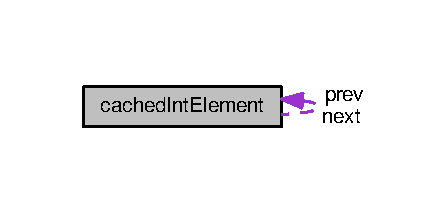
\includegraphics[width=215pt]{structcachedIntElement__coll__graph}
\end{center}
\end{figure}
\subsection*{Public Attributes}
\begin{DoxyCompactItemize}
\item 
uint64\+\_\+t {\bfseries id}\hypertarget{structcachedIntElement_acda821458cfe34dda3bff8b7b0373fb9}{}\label{structcachedIntElement_acda821458cfe34dda3bff8b7b0373fb9}

\item 
uint64\+\_\+t {\bfseries hash}\hypertarget{structcachedIntElement_a20d62592d37c7e8c91449f534431aeb9}{}\label{structcachedIntElement_a20d62592d37c7e8c91449f534431aeb9}

\item 
\hyperlink{structcachedIntElement}{cached\+Int\+Element} $\ast$ {\bfseries next}\hypertarget{structcachedIntElement_ae64f5fae8aa27243af30ef13cb3ebce6}{}\label{structcachedIntElement_ae64f5fae8aa27243af30ef13cb3ebce6}

\item 
\hyperlink{structcachedIntElement}{cached\+Int\+Element} $\ast$ {\bfseries prev}\hypertarget{structcachedIntElement_a90b30c8883b80e42fbf59fbc1bc8727a}{}\label{structcachedIntElement_a90b30c8883b80e42fbf59fbc1bc8727a}

\end{DoxyCompactItemize}


The documentation for this struct was generated from the following file\+:\begin{DoxyCompactItemize}
\item 
hashtable.\+h\end{DoxyCompactItemize}

\hypertarget{structcachedIntElement__binary}{}\section{cached\+Int\+Element\+\_\+binary Struct Reference}
\label{structcachedIntElement__binary}\index{cached\+Int\+Element\+\_\+binary@{cached\+Int\+Element\+\_\+binary}}


element of hash table binary mapping  




{\ttfamily \#include $<$hashtable.\+h$>$}



Collaboration diagram for cached\+Int\+Element\+\_\+binary\+:\nopagebreak
\begin{figure}[H]
\begin{center}
\leavevmode
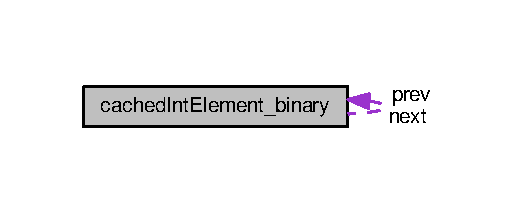
\includegraphics[width=247pt]{structcachedIntElement__binary__coll__graph}
\end{center}
\end{figure}
\subsection*{Public Attributes}
\begin{DoxyCompactItemize}
\item 
uint64\+\_\+t \hyperlink{structcachedIntElement__binary_aa4305da16240730699f33560c0f5aef0}{op1}
\item 
uint64\+\_\+t \hyperlink{structcachedIntElement__binary_aff3a2ddce9bbb4e3e9c8621da7f23799}{op2}
\item 
uint64\+\_\+t \hyperlink{structcachedIntElement__binary_a44ef9752977222f618137d8c1d6d4159}{result}
\item 
uint64\+\_\+t \hyperlink{structcachedIntElement__binary_a61b3637cb5d56531c17cc07aff0b8f84}{extra\+\_\+info}
\item 
uint64\+\_\+t \hyperlink{structcachedIntElement__binary_ad9d23892ecafef09a352699e01aebecc}{hash}
\item 
\hyperlink{structcachedIntElement__binary}{cached\+Int\+Element\+\_\+binary} $\ast$ \hyperlink{structcachedIntElement__binary_a500da0d9af2a1138003bf6b6f0c22555}{next}
\item 
\hyperlink{structcachedIntElement__binary}{cached\+Int\+Element\+\_\+binary} $\ast$ \hyperlink{structcachedIntElement__binary_ae0a95ff1f3a3062e706d06877014e8a6}{prev}
\end{DoxyCompactItemize}


\subsection{Detailed Description}
element of hash table binary mapping 

\subsection{Member Data Documentation}
\index{cached\+Int\+Element\+\_\+binary@{cached\+Int\+Element\+\_\+binary}!extra\+\_\+info@{extra\+\_\+info}}
\index{extra\+\_\+info@{extra\+\_\+info}!cached\+Int\+Element\+\_\+binary@{cached\+Int\+Element\+\_\+binary}}
\subsubsection[{\texorpdfstring{extra\+\_\+info}{extra_info}}]{\setlength{\rightskip}{0pt plus 5cm}uint64\+\_\+t cached\+Int\+Element\+\_\+binary\+::extra\+\_\+info}\hypertarget{structcachedIntElement__binary_a61b3637cb5d56531c17cc07aff0b8f84}{}\label{structcachedIntElement__binary_a61b3637cb5d56531c17cc07aff0b8f84}
id of extra information (e.\+g. rest of division) \index{cached\+Int\+Element\+\_\+binary@{cached\+Int\+Element\+\_\+binary}!hash@{hash}}
\index{hash@{hash}!cached\+Int\+Element\+\_\+binary@{cached\+Int\+Element\+\_\+binary}}
\subsubsection[{\texorpdfstring{hash}{hash}}]{\setlength{\rightskip}{0pt plus 5cm}uint64\+\_\+t cached\+Int\+Element\+\_\+binary\+::hash}\hypertarget{structcachedIntElement__binary_ad9d23892ecafef09a352699e01aebecc}{}\label{structcachedIntElement__binary_ad9d23892ecafef09a352699e01aebecc}
hashed element \index{cached\+Int\+Element\+\_\+binary@{cached\+Int\+Element\+\_\+binary}!next@{next}}
\index{next@{next}!cached\+Int\+Element\+\_\+binary@{cached\+Int\+Element\+\_\+binary}}
\subsubsection[{\texorpdfstring{next}{next}}]{\setlength{\rightskip}{0pt plus 5cm}{\bf cached\+Int\+Element\+\_\+binary}$\ast$ cached\+Int\+Element\+\_\+binary\+::next}\hypertarget{structcachedIntElement__binary_a500da0d9af2a1138003bf6b6f0c22555}{}\label{structcachedIntElement__binary_a500da0d9af2a1138003bf6b6f0c22555}
next element in list \index{cached\+Int\+Element\+\_\+binary@{cached\+Int\+Element\+\_\+binary}!op1@{op1}}
\index{op1@{op1}!cached\+Int\+Element\+\_\+binary@{cached\+Int\+Element\+\_\+binary}}
\subsubsection[{\texorpdfstring{op1}{op1}}]{\setlength{\rightskip}{0pt plus 5cm}uint64\+\_\+t cached\+Int\+Element\+\_\+binary\+::op1}\hypertarget{structcachedIntElement__binary_aa4305da16240730699f33560c0f5aef0}{}\label{structcachedIntElement__binary_aa4305da16240730699f33560c0f5aef0}
id of operator 1 in singleton cache \index{cached\+Int\+Element\+\_\+binary@{cached\+Int\+Element\+\_\+binary}!op2@{op2}}
\index{op2@{op2}!cached\+Int\+Element\+\_\+binary@{cached\+Int\+Element\+\_\+binary}}
\subsubsection[{\texorpdfstring{op2}{op2}}]{\setlength{\rightskip}{0pt plus 5cm}uint64\+\_\+t cached\+Int\+Element\+\_\+binary\+::op2}\hypertarget{structcachedIntElement__binary_aff3a2ddce9bbb4e3e9c8621da7f23799}{}\label{structcachedIntElement__binary_aff3a2ddce9bbb4e3e9c8621da7f23799}
id of operator 2 in singleton cache \index{cached\+Int\+Element\+\_\+binary@{cached\+Int\+Element\+\_\+binary}!prev@{prev}}
\index{prev@{prev}!cached\+Int\+Element\+\_\+binary@{cached\+Int\+Element\+\_\+binary}}
\subsubsection[{\texorpdfstring{prev}{prev}}]{\setlength{\rightskip}{0pt plus 5cm}{\bf cached\+Int\+Element\+\_\+binary}$\ast$ cached\+Int\+Element\+\_\+binary\+::prev}\hypertarget{structcachedIntElement__binary_ae0a95ff1f3a3062e706d06877014e8a6}{}\label{structcachedIntElement__binary_ae0a95ff1f3a3062e706d06877014e8a6}
previous element in list \index{cached\+Int\+Element\+\_\+binary@{cached\+Int\+Element\+\_\+binary}!result@{result}}
\index{result@{result}!cached\+Int\+Element\+\_\+binary@{cached\+Int\+Element\+\_\+binary}}
\subsubsection[{\texorpdfstring{result}{result}}]{\setlength{\rightskip}{0pt plus 5cm}uint64\+\_\+t cached\+Int\+Element\+\_\+binary\+::result}\hypertarget{structcachedIntElement__binary_a44ef9752977222f618137d8c1d6d4159}{}\label{structcachedIntElement__binary_a44ef9752977222f618137d8c1d6d4159}
id of result in singleton cache 

The documentation for this struct was generated from the following file\+:\begin{DoxyCompactItemize}
\item 
\hyperlink{hashtable_8h}{hashtable.\+h}\end{DoxyCompactItemize}

\hypertarget{structcachedIntList}{}\section{cached\+Int\+List Struct Reference}
\label{structcachedIntList}\index{cached\+Int\+List@{cached\+Int\+List}}


Collaboration diagram for cached\+Int\+List\+:
\nopagebreak
\begin{figure}[H]
\begin{center}
\leavevmode
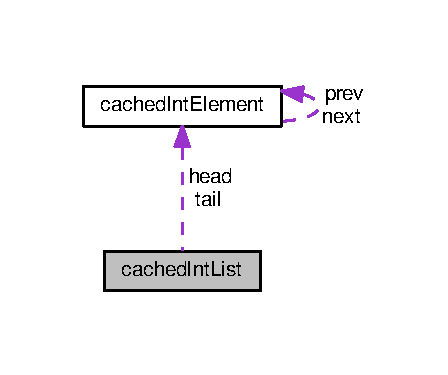
\includegraphics[width=215pt]{structcachedIntList__coll__graph}
\end{center}
\end{figure}
\subsection*{Public Attributes}
\begin{DoxyCompactItemize}
\item 
\hyperlink{structcachedIntElement}{cached\+Int\+Element} $\ast$ {\bfseries head}\hypertarget{structcachedIntList_ac4cce5e5d07c4b23683046e77a0fbe6a}{}\label{structcachedIntList_ac4cce5e5d07c4b23683046e77a0fbe6a}

\item 
\hyperlink{structcachedIntElement}{cached\+Int\+Element} $\ast$ {\bfseries tail}\hypertarget{structcachedIntList_adbe1df126c4425546e3a2b4366784c9d}{}\label{structcachedIntList_adbe1df126c4425546e3a2b4366784c9d}

\end{DoxyCompactItemize}


The documentation for this struct was generated from the following file\+:\begin{DoxyCompactItemize}
\item 
hashtable.\+h\end{DoxyCompactItemize}

\hypertarget{structcachedIntList__binary}{}\section{cached\+Int\+List\+\_\+binary Struct Reference}
\label{structcachedIntList__binary}\index{cached\+Int\+List\+\_\+binary@{cached\+Int\+List\+\_\+binary}}


list of elements in one slot of the hash table binary mapping  




{\ttfamily \#include $<$hashtable.\+h$>$}



Collaboration diagram for cached\+Int\+List\+\_\+binary\+:\nopagebreak
\begin{figure}[H]
\begin{center}
\leavevmode
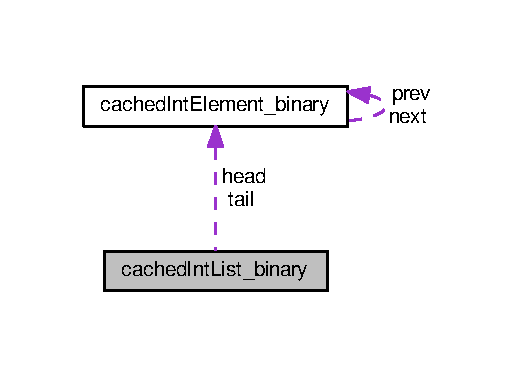
\includegraphics[width=247pt]{structcachedIntList__binary__coll__graph}
\end{center}
\end{figure}
\subsection*{Public Attributes}
\begin{DoxyCompactItemize}
\item 
\hyperlink{structcachedIntElement__binary}{cached\+Int\+Element\+\_\+binary} $\ast$ \hyperlink{structcachedIntList__binary_ab51ea19cb68af38612cad45b08d9239f}{head}
\item 
\hyperlink{structcachedIntElement__binary}{cached\+Int\+Element\+\_\+binary} $\ast$ \hyperlink{structcachedIntList__binary_ad92905f1242fc89c700572d0d510c17f}{tail}
\end{DoxyCompactItemize}


\subsection{Detailed Description}
list of elements in one slot of the hash table binary mapping 

\subsection{Member Data Documentation}
\index{cached\+Int\+List\+\_\+binary@{cached\+Int\+List\+\_\+binary}!head@{head}}
\index{head@{head}!cached\+Int\+List\+\_\+binary@{cached\+Int\+List\+\_\+binary}}
\subsubsection[{\texorpdfstring{head}{head}}]{\setlength{\rightskip}{0pt plus 5cm}{\bf cached\+Int\+Element\+\_\+binary}$\ast$ cached\+Int\+List\+\_\+binary\+::head}\hypertarget{structcachedIntList__binary_ab51ea19cb68af38612cad45b08d9239f}{}\label{structcachedIntList__binary_ab51ea19cb68af38612cad45b08d9239f}
head pointer of list \index{cached\+Int\+List\+\_\+binary@{cached\+Int\+List\+\_\+binary}!tail@{tail}}
\index{tail@{tail}!cached\+Int\+List\+\_\+binary@{cached\+Int\+List\+\_\+binary}}
\subsubsection[{\texorpdfstring{tail}{tail}}]{\setlength{\rightskip}{0pt plus 5cm}{\bf cached\+Int\+Element\+\_\+binary}$\ast$ cached\+Int\+List\+\_\+binary\+::tail}\hypertarget{structcachedIntList__binary_ad92905f1242fc89c700572d0d510c17f}{}\label{structcachedIntList__binary_ad92905f1242fc89c700572d0d510c17f}
tail pointer of list for fast insert 

The documentation for this struct was generated from the following file\+:\begin{DoxyCompactItemize}
\item 
\hyperlink{hashtable_8h}{hashtable.\+h}\end{DoxyCompactItemize}

\hypertarget{structcachedRational}{}\section{cached\+Rational Struct Reference}
\label{structcachedRational}\index{cached\+Rational@{cached\+Rational}}
\subsection*{Public Attributes}
\begin{DoxyCompactItemize}
\item 
cache\+\_\+mpq \hyperlink{structcachedRational_af4bc91012e94d43c4f50e15db3a6b4ea}{counter}
\item 
cache\+\_\+mpq \hyperlink{structcachedRational_a319e0c2eb1d91bcb7cd04a32c7a8dbb7}{denominator}
\end{DoxyCompactItemize}


\subsection{Detailed Description}
cached Rational 

\subsection{Member Data Documentation}
\index{cached\+Rational@{cached\+Rational}!counter@{counter}}
\index{counter@{counter}!cached\+Rational@{cached\+Rational}}
\subsubsection[{\texorpdfstring{counter}{counter}}]{\setlength{\rightskip}{0pt plus 5cm}cache\+\_\+mpq cached\+Rational\+::counter}\hypertarget{structcachedRational_af4bc91012e94d43c4f50e15db3a6b4ea}{}\label{structcachedRational_af4bc91012e94d43c4f50e15db3a6b4ea}
counter \index{cached\+Rational@{cached\+Rational}!denominator@{denominator}}
\index{denominator@{denominator}!cached\+Rational@{cached\+Rational}}
\subsubsection[{\texorpdfstring{denominator}{denominator}}]{\setlength{\rightskip}{0pt plus 5cm}cache\+\_\+mpq cached\+Rational\+::denominator}\hypertarget{structcachedRational_a319e0c2eb1d91bcb7cd04a32c7a8dbb7}{}\label{structcachedRational_a319e0c2eb1d91bcb7cd04a32c7a8dbb7}
denominator 

The documentation for this struct was generated from the following file\+:\begin{DoxyCompactItemize}
\item 
master\+\_\+cache\+\_\+rational.\+c\end{DoxyCompactItemize}

\hypertarget{structHashtable}{}\section{Hashtable Struct Reference}
\label{structHashtable}\index{Hashtable@{Hashtable}}


hash table  




{\ttfamily \#include $<$hashtable.\+h$>$}



Collaboration diagram for Hashtable\+:\nopagebreak
\begin{figure}[H]
\begin{center}
\leavevmode
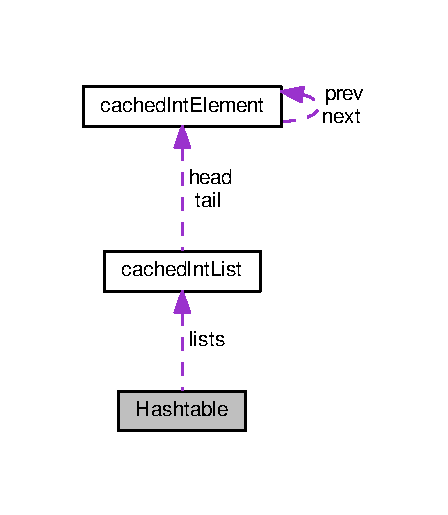
\includegraphics[width=215pt]{structHashtable__coll__graph}
\end{center}
\end{figure}
\subsection*{Public Attributes}
\begin{DoxyCompactItemize}
\item 
int $\ast$ \hyperlink{structHashtable_a99f7c11aa20bbd066528843438a42958}{counter}
\item 
\hyperlink{structcachedIntList}{cached\+Int\+List} $\ast$ \hyperlink{structHashtable_ac4140ebb0209a40547999cce896fe17c}{lists}
\item 
uint64\+\_\+t \hyperlink{structHashtable_aab81586954ce81cc3d52b41cf5ec5a04}{size}
\end{DoxyCompactItemize}


\subsection{Detailed Description}
hash table 

\subsection{Member Data Documentation}
\index{Hashtable@{Hashtable}!counter@{counter}}
\index{counter@{counter}!Hashtable@{Hashtable}}
\subsubsection[{\texorpdfstring{counter}{counter}}]{\setlength{\rightskip}{0pt plus 5cm}int$\ast$ Hashtable\+::counter}\hypertarget{structHashtable_a99f7c11aa20bbd066528843438a42958}{}\label{structHashtable_a99f7c11aa20bbd066528843438a42958}
array of counters of elements in each list \index{Hashtable@{Hashtable}!lists@{lists}}
\index{lists@{lists}!Hashtable@{Hashtable}}
\subsubsection[{\texorpdfstring{lists}{lists}}]{\setlength{\rightskip}{0pt plus 5cm}{\bf cached\+Int\+List}$\ast$ Hashtable\+::lists}\hypertarget{structHashtable_ac4140ebb0209a40547999cce896fe17c}{}\label{structHashtable_ac4140ebb0209a40547999cce896fe17c}
array of lists \index{Hashtable@{Hashtable}!size@{size}}
\index{size@{size}!Hashtable@{Hashtable}}
\subsubsection[{\texorpdfstring{size}{size}}]{\setlength{\rightskip}{0pt plus 5cm}uint64\+\_\+t Hashtable\+::size}\hypertarget{structHashtable_aab81586954ce81cc3d52b41cf5ec5a04}{}\label{structHashtable_aab81586954ce81cc3d52b41cf5ec5a04}
number of lists, size of hash table 

The documentation for this struct was generated from the following file\+:\begin{DoxyCompactItemize}
\item 
\hyperlink{hashtable_8h}{hashtable.\+h}\end{DoxyCompactItemize}

\hypertarget{structHashtable__binary}{}\section{Hashtable\+\_\+binary Struct Reference}
\label{structHashtable__binary}\index{Hashtable\+\_\+binary@{Hashtable\+\_\+binary}}


hash table binary mapping  




{\ttfamily \#include $<$hashtable.\+h$>$}



Collaboration diagram for Hashtable\+\_\+binary\+:\nopagebreak
\begin{figure}[H]
\begin{center}
\leavevmode
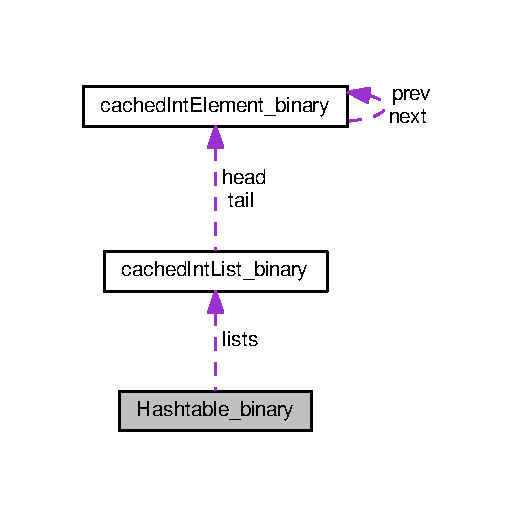
\includegraphics[width=247pt]{structHashtable__binary__coll__graph}
\end{center}
\end{figure}
\subsection*{Public Attributes}
\begin{DoxyCompactItemize}
\item 
int $\ast$ \hyperlink{structHashtable__binary_a84f8baf046a4f7a75a405e8fd448bac8}{counter}
\item 
\hyperlink{structcachedIntList__binary}{cached\+Int\+List\+\_\+binary} $\ast$ \hyperlink{structHashtable__binary_a6c33200915e4022c6c561f35fc36d4e0}{lists}
\item 
uint64\+\_\+t \hyperlink{structHashtable__binary_a2232ebf98285e8d0154badb1db51fdc5}{size}
\end{DoxyCompactItemize}


\subsection{Detailed Description}
hash table binary mapping 

\subsection{Member Data Documentation}
\index{Hashtable\+\_\+binary@{Hashtable\+\_\+binary}!counter@{counter}}
\index{counter@{counter}!Hashtable\+\_\+binary@{Hashtable\+\_\+binary}}
\subsubsection[{\texorpdfstring{counter}{counter}}]{\setlength{\rightskip}{0pt plus 5cm}int$\ast$ Hashtable\+\_\+binary\+::counter}\hypertarget{structHashtable__binary_a84f8baf046a4f7a75a405e8fd448bac8}{}\label{structHashtable__binary_a84f8baf046a4f7a75a405e8fd448bac8}
array of counters of elements in each list \index{Hashtable\+\_\+binary@{Hashtable\+\_\+binary}!lists@{lists}}
\index{lists@{lists}!Hashtable\+\_\+binary@{Hashtable\+\_\+binary}}
\subsubsection[{\texorpdfstring{lists}{lists}}]{\setlength{\rightskip}{0pt plus 5cm}{\bf cached\+Int\+List\+\_\+binary}$\ast$ Hashtable\+\_\+binary\+::lists}\hypertarget{structHashtable__binary_a6c33200915e4022c6c561f35fc36d4e0}{}\label{structHashtable__binary_a6c33200915e4022c6c561f35fc36d4e0}
array of lists \index{Hashtable\+\_\+binary@{Hashtable\+\_\+binary}!size@{size}}
\index{size@{size}!Hashtable\+\_\+binary@{Hashtable\+\_\+binary}}
\subsubsection[{\texorpdfstring{size}{size}}]{\setlength{\rightskip}{0pt plus 5cm}uint64\+\_\+t Hashtable\+\_\+binary\+::size}\hypertarget{structHashtable__binary_a2232ebf98285e8d0154badb1db51fdc5}{}\label{structHashtable__binary_a2232ebf98285e8d0154badb1db51fdc5}
number of lists, size of hash table 

The documentation for this struct was generated from the following file\+:\begin{DoxyCompactItemize}
\item 
\hyperlink{hashtable_8h}{hashtable.\+h}\end{DoxyCompactItemize}

\hypertarget{structlookup}{}\section{lookup Struct Reference}
\label{structlookup}\index{lookup@{lookup}}


collection of lookup tables for the required operations  




{\ttfamily \#include $<$caching\+\_\+operations.\+h$>$}



Collaboration diagram for lookup\+:\nopagebreak
\begin{figure}[H]
\begin{center}
\leavevmode
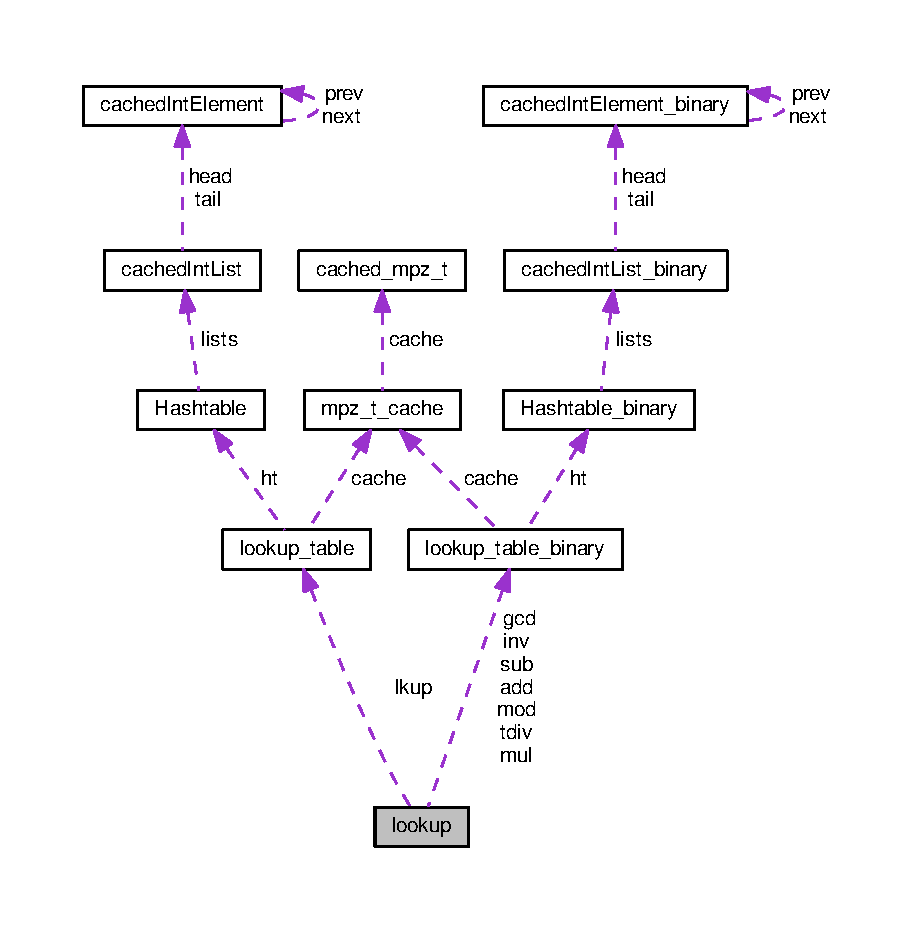
\includegraphics[width=350pt]{structlookup__coll__graph}
\end{center}
\end{figure}
\subsection*{Public Attributes}
\begin{DoxyCompactItemize}
\item 
\hyperlink{structlookup__table}{lookup\+\_\+table} $\ast$ \hyperlink{structlookup_aac4b32e67de7870ed7ef9da8077faf3d}{lkup}
\item 
\hyperlink{structlookup__table__binary}{lookup\+\_\+table\+\_\+binary} $\ast$ \hyperlink{structlookup_ada52eb4221d2d2ab592f13e57936dad2}{add}
\item 
\hyperlink{structlookup__table__binary}{lookup\+\_\+table\+\_\+binary} $\ast$ \hyperlink{structlookup_a6847e05562a081e06e25d33ac8a205a2}{sub}
\item 
\hyperlink{structlookup__table__binary}{lookup\+\_\+table\+\_\+binary} $\ast$ \hyperlink{structlookup_aab703d9a300ea104f80a39416e512041}{mul}
\item 
\hyperlink{structlookup__table__binary}{lookup\+\_\+table\+\_\+binary} $\ast$ \hyperlink{structlookup_abef492b10c81737d02dae892da38719a}{tdiv}
\item 
\hyperlink{structlookup__table__binary}{lookup\+\_\+table\+\_\+binary} $\ast$ \hyperlink{structlookup_aec682b8433afc9c027849a48f051af95}{mod}
\item 
\hyperlink{structlookup__table__binary}{lookup\+\_\+table\+\_\+binary} $\ast$ \hyperlink{structlookup_aaadaeeb9f694301aec3fe2c275c6201f}{gcd}
\item 
\hyperlink{structlookup__table__binary}{lookup\+\_\+table\+\_\+binary} $\ast$ \hyperlink{structlookup_aad2f4d538e0e689ac57e456b65f36913}{inv}
\end{DoxyCompactItemize}


\subsection{Detailed Description}
collection of lookup tables for the required operations 

\subsection{Member Data Documentation}
\index{lookup@{lookup}!add@{add}}
\index{add@{add}!lookup@{lookup}}
\subsubsection[{\texorpdfstring{add}{add}}]{\setlength{\rightskip}{0pt plus 5cm}{\bf lookup\+\_\+table\+\_\+binary}$\ast$ lookup\+::add}\hypertarget{structlookup_ada52eb4221d2d2ab592f13e57936dad2}{}\label{structlookup_ada52eb4221d2d2ab592f13e57936dad2}
lookup table for mpz\+\_\+t addition \index{lookup@{lookup}!gcd@{gcd}}
\index{gcd@{gcd}!lookup@{lookup}}
\subsubsection[{\texorpdfstring{gcd}{gcd}}]{\setlength{\rightskip}{0pt plus 5cm}{\bf lookup\+\_\+table\+\_\+binary}$\ast$ lookup\+::gcd}\hypertarget{structlookup_aaadaeeb9f694301aec3fe2c275c6201f}{}\label{structlookup_aaadaeeb9f694301aec3fe2c275c6201f}
lookup table for mpz\+\_\+t greatest common divisor \index{lookup@{lookup}!inv@{inv}}
\index{inv@{inv}!lookup@{lookup}}
\subsubsection[{\texorpdfstring{inv}{inv}}]{\setlength{\rightskip}{0pt plus 5cm}{\bf lookup\+\_\+table\+\_\+binary}$\ast$ lookup\+::inv}\hypertarget{structlookup_aad2f4d538e0e689ac57e456b65f36913}{}\label{structlookup_aad2f4d538e0e689ac57e456b65f36913}
lookup table for mpz\+\_\+t modular multiplicative inverse \index{lookup@{lookup}!lkup@{lkup}}
\index{lkup@{lkup}!lookup@{lookup}}
\subsubsection[{\texorpdfstring{lkup}{lkup}}]{\setlength{\rightskip}{0pt plus 5cm}{\bf lookup\+\_\+table}$\ast$ lookup\+::lkup}\hypertarget{structlookup_aac4b32e67de7870ed7ef9da8077faf3d}{}\label{structlookup_aac4b32e67de7870ed7ef9da8077faf3d}
lookup table for mpz\+\_\+t \index{lookup@{lookup}!mod@{mod}}
\index{mod@{mod}!lookup@{lookup}}
\subsubsection[{\texorpdfstring{mod}{mod}}]{\setlength{\rightskip}{0pt plus 5cm}{\bf lookup\+\_\+table\+\_\+binary}$\ast$ lookup\+::mod}\hypertarget{structlookup_aec682b8433afc9c027849a48f051af95}{}\label{structlookup_aec682b8433afc9c027849a48f051af95}
lookup table for mpz\+\_\+t modulo \index{lookup@{lookup}!mul@{mul}}
\index{mul@{mul}!lookup@{lookup}}
\subsubsection[{\texorpdfstring{mul}{mul}}]{\setlength{\rightskip}{0pt plus 5cm}{\bf lookup\+\_\+table\+\_\+binary}$\ast$ lookup\+::mul}\hypertarget{structlookup_aab703d9a300ea104f80a39416e512041}{}\label{structlookup_aab703d9a300ea104f80a39416e512041}
lookup table for mpz\+\_\+t multiplication \index{lookup@{lookup}!sub@{sub}}
\index{sub@{sub}!lookup@{lookup}}
\subsubsection[{\texorpdfstring{sub}{sub}}]{\setlength{\rightskip}{0pt plus 5cm}{\bf lookup\+\_\+table\+\_\+binary}$\ast$ lookup\+::sub}\hypertarget{structlookup_a6847e05562a081e06e25d33ac8a205a2}{}\label{structlookup_a6847e05562a081e06e25d33ac8a205a2}
lookup table for mpz\+\_\+t subtraction \index{lookup@{lookup}!tdiv@{tdiv}}
\index{tdiv@{tdiv}!lookup@{lookup}}
\subsubsection[{\texorpdfstring{tdiv}{tdiv}}]{\setlength{\rightskip}{0pt plus 5cm}{\bf lookup\+\_\+table\+\_\+binary}$\ast$ lookup\+::tdiv}\hypertarget{structlookup_abef492b10c81737d02dae892da38719a}{}\label{structlookup_abef492b10c81737d02dae892da38719a}
lookup table for mpz\+\_\+t integer division 

The documentation for this struct was generated from the following file\+:\begin{DoxyCompactItemize}
\item 
\hyperlink{caching__operations_8h}{caching\+\_\+operations.\+h}\end{DoxyCompactItemize}

\hypertarget{structlookup__table}{}\section{lookup\+\_\+table Struct Reference}
\label{structlookup__table}\index{lookup\+\_\+table@{lookup\+\_\+table}}


lookup table for mpz\+\_\+t  




{\ttfamily \#include $<$caching\+\_\+operations.\+h$>$}



Collaboration diagram for lookup\+\_\+table\+:\nopagebreak
\begin{figure}[H]
\begin{center}
\leavevmode
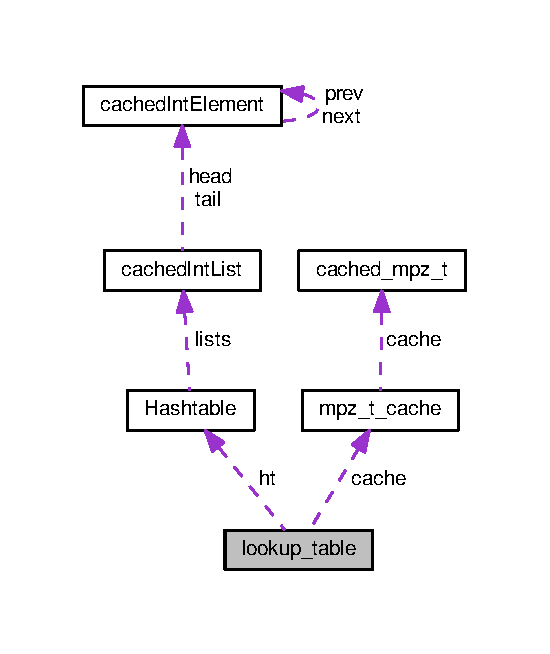
\includegraphics[width=264pt]{structlookup__table__coll__graph}
\end{center}
\end{figure}
\subsection*{Public Attributes}
\begin{DoxyCompactItemize}
\item 
\hyperlink{structHashtable}{Hashtable} $\ast$ \hyperlink{structlookup__table_a2066d36e3a0f245e7f428f1e951cd947}{ht}
\item 
\hyperlink{structmpz__t__cache}{mpz\+\_\+t\+\_\+cache} $\ast$ \hyperlink{structlookup__table_a120547b02b115a402c758cf630ed22b1}{cache}
\end{DoxyCompactItemize}


\subsection{Detailed Description}
lookup table for mpz\+\_\+t 

\subsection{Member Data Documentation}
\index{lookup\+\_\+table@{lookup\+\_\+table}!cache@{cache}}
\index{cache@{cache}!lookup\+\_\+table@{lookup\+\_\+table}}
\subsubsection[{\texorpdfstring{cache}{cache}}]{\setlength{\rightskip}{0pt plus 5cm}{\bf mpz\+\_\+t\+\_\+cache}$\ast$ lookup\+\_\+table\+::cache}\hypertarget{structlookup__table_a120547b02b115a402c758cf630ed22b1}{}\label{structlookup__table_a120547b02b115a402c758cf630ed22b1}
pointer to singleton mpz\+\_\+t cache \index{lookup\+\_\+table@{lookup\+\_\+table}!ht@{ht}}
\index{ht@{ht}!lookup\+\_\+table@{lookup\+\_\+table}}
\subsubsection[{\texorpdfstring{ht}{ht}}]{\setlength{\rightskip}{0pt plus 5cm}{\bf Hashtable}$\ast$ lookup\+\_\+table\+::ht}\hypertarget{structlookup__table_a2066d36e3a0f245e7f428f1e951cd947}{}\label{structlookup__table_a2066d36e3a0f245e7f428f1e951cd947}
hash table for mpz\+\_\+t 

The documentation for this struct was generated from the following file\+:\begin{DoxyCompactItemize}
\item 
\hyperlink{caching__operations_8h}{caching\+\_\+operations.\+h}\end{DoxyCompactItemize}

\hypertarget{structlookup__table__binary}{}\section{lookup\+\_\+table\+\_\+binary Struct Reference}
\label{structlookup__table__binary}\index{lookup\+\_\+table\+\_\+binary@{lookup\+\_\+table\+\_\+binary}}


lookup table for binary operations mpz\+\_\+t x mpz\+\_\+t -\/$>$ mpz\+\_\+t  




{\ttfamily \#include $<$caching\+\_\+operations.\+h$>$}



Collaboration diagram for lookup\+\_\+table\+\_\+binary\+:\nopagebreak
\begin{figure}[H]
\begin{center}
\leavevmode
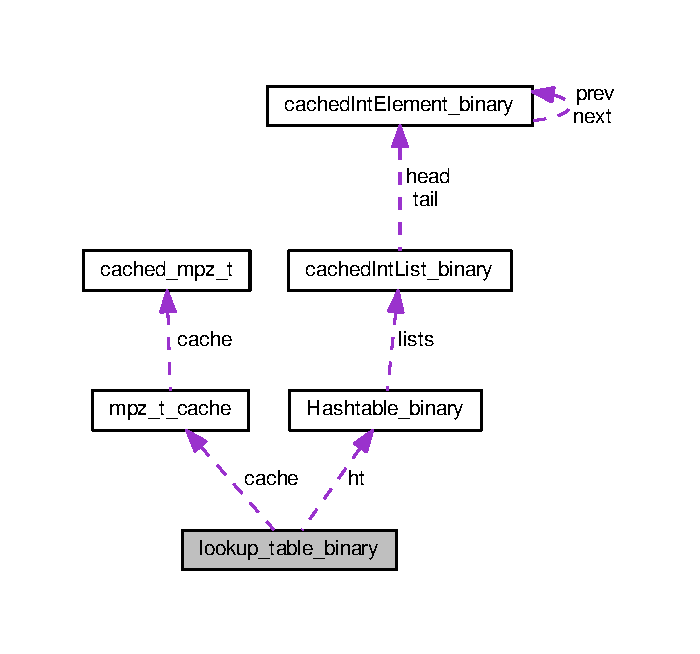
\includegraphics[width=336pt]{structlookup__table__binary__coll__graph}
\end{center}
\end{figure}
\subsection*{Public Attributes}
\begin{DoxyCompactItemize}
\item 
\hyperlink{structHashtable__binary}{Hashtable\+\_\+binary} $\ast$ \hyperlink{structlookup__table__binary_ae12894f1b36d77b08582558701d25029}{ht}
\item 
\hyperlink{structmpz__t__cache}{mpz\+\_\+t\+\_\+cache} $\ast$ \hyperlink{structlookup__table__binary_ad68f0a417fc2f1e237bfc5077d5f68c6}{cache}
\end{DoxyCompactItemize}


\subsection{Detailed Description}
lookup table for binary operations mpz\+\_\+t x mpz\+\_\+t -\/$>$ mpz\+\_\+t 

\subsection{Member Data Documentation}
\index{lookup\+\_\+table\+\_\+binary@{lookup\+\_\+table\+\_\+binary}!cache@{cache}}
\index{cache@{cache}!lookup\+\_\+table\+\_\+binary@{lookup\+\_\+table\+\_\+binary}}
\subsubsection[{\texorpdfstring{cache}{cache}}]{\setlength{\rightskip}{0pt plus 5cm}{\bf mpz\+\_\+t\+\_\+cache}$\ast$ lookup\+\_\+table\+\_\+binary\+::cache}\hypertarget{structlookup__table__binary_ad68f0a417fc2f1e237bfc5077d5f68c6}{}\label{structlookup__table__binary_ad68f0a417fc2f1e237bfc5077d5f68c6}
pointer to singleton mpz\+\_\+t cache \index{lookup\+\_\+table\+\_\+binary@{lookup\+\_\+table\+\_\+binary}!ht@{ht}}
\index{ht@{ht}!lookup\+\_\+table\+\_\+binary@{lookup\+\_\+table\+\_\+binary}}
\subsubsection[{\texorpdfstring{ht}{ht}}]{\setlength{\rightskip}{0pt plus 5cm}{\bf Hashtable\+\_\+binary}$\ast$ lookup\+\_\+table\+\_\+binary\+::ht}\hypertarget{structlookup__table__binary_ae12894f1b36d77b08582558701d25029}{}\label{structlookup__table__binary_ae12894f1b36d77b08582558701d25029}
hash table for (mpz\+\_\+t x mpz\+\_\+t) 

The documentation for this struct was generated from the following file\+:\begin{DoxyCompactItemize}
\item 
\hyperlink{caching__operations_8h}{caching\+\_\+operations.\+h}\end{DoxyCompactItemize}

\hypertarget{structMasterCache}{}\section{Master\+Cache Struct Reference}
\label{structMasterCache}\index{Master\+Cache@{Master\+Cache}}


\hyperlink{structMasterCache}{Master\+Cache}.  




{\ttfamily \#include $<$mastercache.\+h$>$}



Collaboration diagram for Master\+Cache\+:\nopagebreak
\begin{figure}[H]
\begin{center}
\leavevmode
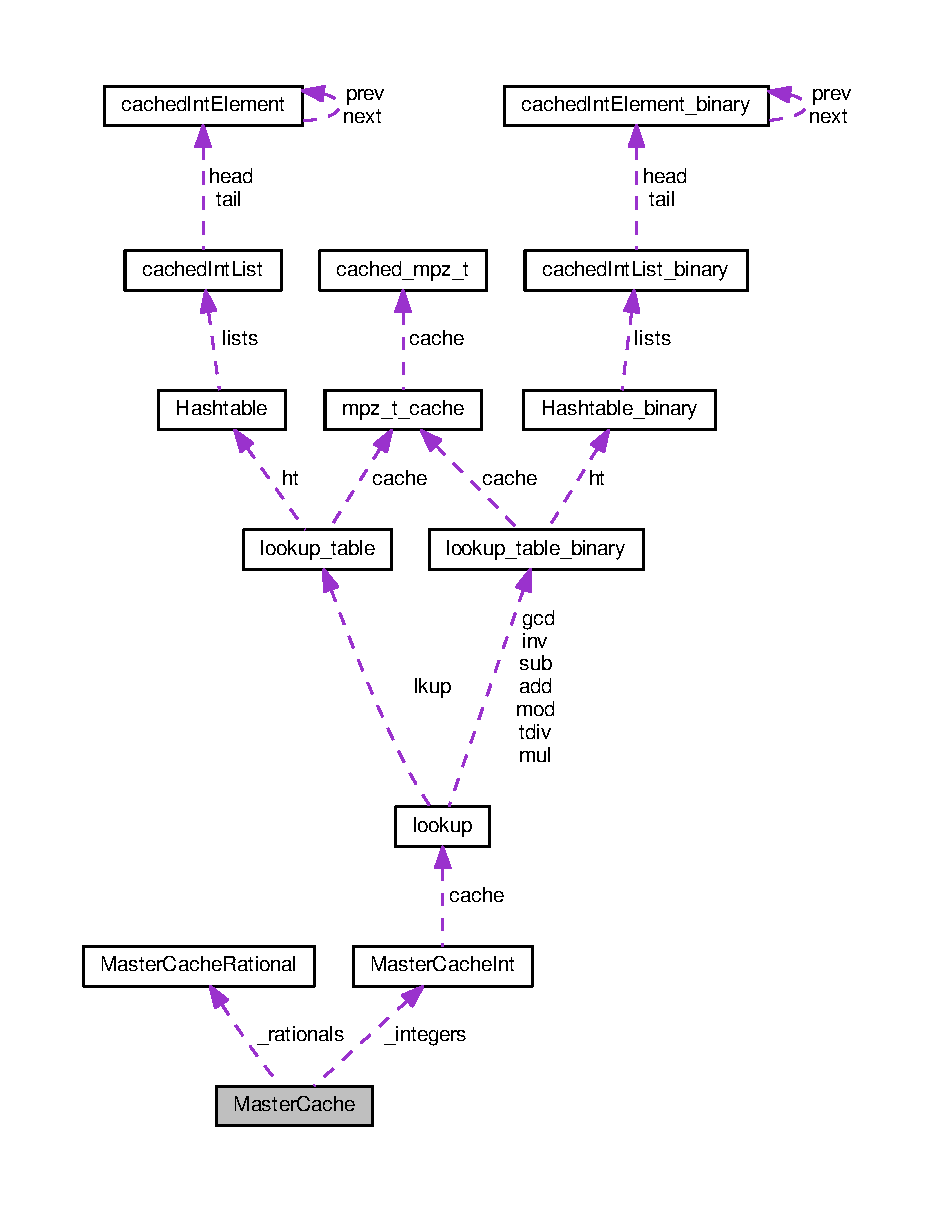
\includegraphics[width=350pt]{structMasterCache__coll__graph}
\end{center}
\end{figure}
\subsection*{Public Attributes}
\begin{DoxyCompactItemize}
\item 
\hyperlink{structMasterCacheInt}{Master\+Cache\+Int} $\ast$ \hyperlink{structMasterCache_a5c3a0aa848b8d98114902f674e111dc3}{\+\_\+integers}
\item 
\hyperlink{structMasterCacheRational}{Master\+Cache\+Rational} $\ast$ \hyperlink{structMasterCache_a2cc414dcdfc90d3841ffa329f0877f67}{\+\_\+rationals}
\end{DoxyCompactItemize}


\subsection{Detailed Description}
\hyperlink{structMasterCache}{Master\+Cache}. 

\subsection{Member Data Documentation}
\index{Master\+Cache@{Master\+Cache}!\+\_\+integers@{\+\_\+integers}}
\index{\+\_\+integers@{\+\_\+integers}!Master\+Cache@{Master\+Cache}}
\subsubsection[{\texorpdfstring{\+\_\+integers}{_integers}}]{\setlength{\rightskip}{0pt plus 5cm}{\bf Master\+Cache\+Int}$\ast$ Master\+Cache\+::\+\_\+integers}\hypertarget{structMasterCache_a5c3a0aa848b8d98114902f674e111dc3}{}\label{structMasterCache_a5c3a0aa848b8d98114902f674e111dc3}
cache for integer caching \index{Master\+Cache@{Master\+Cache}!\+\_\+rationals@{\+\_\+rationals}}
\index{\+\_\+rationals@{\+\_\+rationals}!Master\+Cache@{Master\+Cache}}
\subsubsection[{\texorpdfstring{\+\_\+rationals}{_rationals}}]{\setlength{\rightskip}{0pt plus 5cm}{\bf Master\+Cache\+Rational}$\ast$ Master\+Cache\+::\+\_\+rationals}\hypertarget{structMasterCache_a2cc414dcdfc90d3841ffa329f0877f67}{}\label{structMasterCache_a2cc414dcdfc90d3841ffa329f0877f67}
cache for rational caching 

The documentation for this struct was generated from the following file\+:\begin{DoxyCompactItemize}
\item 
\hyperlink{mastercache_8h}{mastercache.\+h}\end{DoxyCompactItemize}

\hypertarget{structMasterCacheInt}{}\section{Master\+Cache\+Int Struct Reference}
\label{structMasterCacheInt}\index{Master\+Cache\+Int@{Master\+Cache\+Int}}


{\ttfamily \#include $<$mastercache.\+h$>$}



Collaboration diagram for Master\+Cache\+Int\+:\nopagebreak
\begin{figure}[H]
\begin{center}
\leavevmode
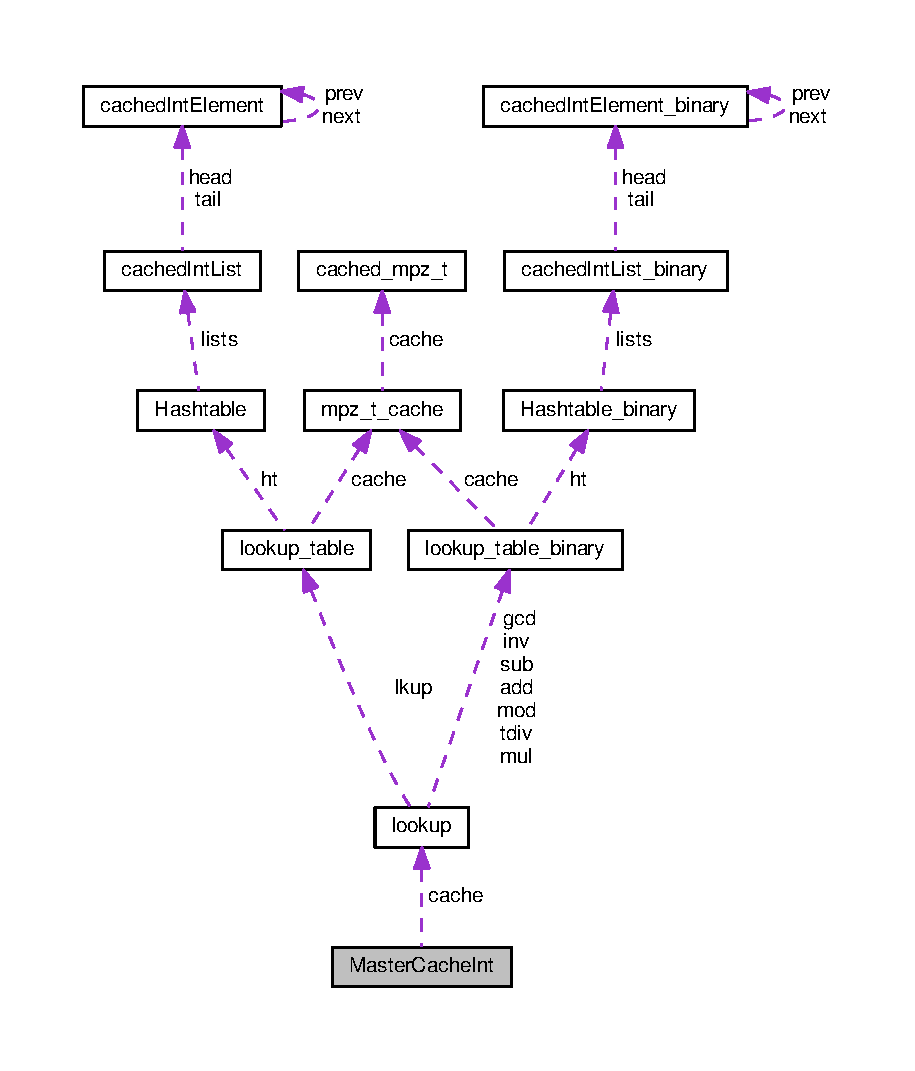
\includegraphics[width=350pt]{structMasterCacheInt__coll__graph}
\end{center}
\end{figure}
\subsection*{Public Attributes}
\begin{DoxyCompactItemize}
\item 
\hyperlink{structlookup}{lookup} $\ast$ \hyperlink{structMasterCacheInt_a4e80ed8be2db43aa586a75118a62606a}{cache}
\end{DoxyCompactItemize}


\subsection{Detailed Description}
Master cache for integers 

\subsection{Member Data Documentation}
\index{Master\+Cache\+Int@{Master\+Cache\+Int}!cache@{cache}}
\index{cache@{cache}!Master\+Cache\+Int@{Master\+Cache\+Int}}
\subsubsection[{\texorpdfstring{cache}{cache}}]{\setlength{\rightskip}{0pt plus 5cm}{\bf lookup}$\ast$ Master\+Cache\+Int\+::cache}\hypertarget{structMasterCacheInt_a4e80ed8be2db43aa586a75118a62606a}{}\label{structMasterCacheInt_a4e80ed8be2db43aa586a75118a62606a}
cache for integer caching 

The documentation for this struct was generated from the following file\+:\begin{DoxyCompactItemize}
\item 
\hyperlink{mastercache_8h}{mastercache.\+h}\end{DoxyCompactItemize}

\hypertarget{structMasterCacheRational}{}\section{Master\+Cache\+Rational Struct Reference}
\label{structMasterCacheRational}\index{Master\+Cache\+Rational@{Master\+Cache\+Rational}}


The documentation for this struct was generated from the following file\+:\begin{DoxyCompactItemize}
\item 
master\+\_\+cache\+\_\+rational.\+c\end{DoxyCompactItemize}

\hypertarget{structmpz__t__cache}{}\section{mpz\+\_\+t\+\_\+cache Struct Reference}
\label{structmpz__t__cache}\index{mpz\+\_\+t\+\_\+cache@{mpz\+\_\+t\+\_\+cache}}


cache implemented as an array (fast random access)  




{\ttfamily \#include $<$mpz\+\_\+caching.\+h$>$}



Collaboration diagram for mpz\+\_\+t\+\_\+cache\+:\nopagebreak
\begin{figure}[H]
\begin{center}
\leavevmode
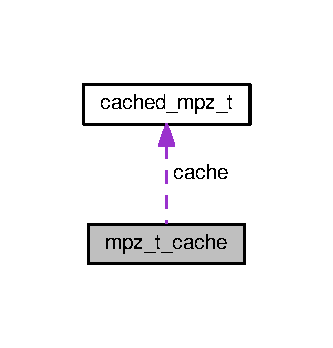
\includegraphics[width=160pt]{structmpz__t__cache__coll__graph}
\end{center}
\end{figure}
\subsection*{Public Attributes}
\begin{DoxyCompactItemize}
\item 
\hyperlink{structcached__mpz__t}{cached\+\_\+mpz\+\_\+t} $\ast$ \hyperlink{structmpz__t__cache_a68ba0b84ae67ae594f539b466dac5008}{cache}
\item 
uint64\+\_\+t \hyperlink{structmpz__t__cache_ad8f52046ab32c2b94ca4a32f22b4beb7}{next\+\_\+id}
\item 
uint64\+\_\+t \hyperlink{structmpz__t__cache_a00982c72af6f0784f31c8d28bb56fbf8}{size}
\end{DoxyCompactItemize}


\subsection{Detailed Description}
cache implemented as an array (fast random access) 

\subsection{Member Data Documentation}
\index{mpz\+\_\+t\+\_\+cache@{mpz\+\_\+t\+\_\+cache}!cache@{cache}}
\index{cache@{cache}!mpz\+\_\+t\+\_\+cache@{mpz\+\_\+t\+\_\+cache}}
\subsubsection[{\texorpdfstring{cache}{cache}}]{\setlength{\rightskip}{0pt plus 5cm}{\bf cached\+\_\+mpz\+\_\+t}$\ast$ mpz\+\_\+t\+\_\+cache\+::cache}\hypertarget{structmpz__t__cache_a68ba0b84ae67ae594f539b466dac5008}{}\label{structmpz__t__cache_a68ba0b84ae67ae594f539b466dac5008}
array of \hyperlink{structcached__mpz__t}{cached\+\_\+mpz\+\_\+t} \index{mpz\+\_\+t\+\_\+cache@{mpz\+\_\+t\+\_\+cache}!next\+\_\+id@{next\+\_\+id}}
\index{next\+\_\+id@{next\+\_\+id}!mpz\+\_\+t\+\_\+cache@{mpz\+\_\+t\+\_\+cache}}
\subsubsection[{\texorpdfstring{next\+\_\+id}{next_id}}]{\setlength{\rightskip}{0pt plus 5cm}uint64\+\_\+t mpz\+\_\+t\+\_\+cache\+::next\+\_\+id}\hypertarget{structmpz__t__cache_ad8f52046ab32c2b94ca4a32f22b4beb7}{}\label{structmpz__t__cache_ad8f52046ab32c2b94ca4a32f22b4beb7}
next free id for fast insert \index{mpz\+\_\+t\+\_\+cache@{mpz\+\_\+t\+\_\+cache}!size@{size}}
\index{size@{size}!mpz\+\_\+t\+\_\+cache@{mpz\+\_\+t\+\_\+cache}}
\subsubsection[{\texorpdfstring{size}{size}}]{\setlength{\rightskip}{0pt plus 5cm}uint64\+\_\+t mpz\+\_\+t\+\_\+cache\+::size}\hypertarget{structmpz__t__cache_a00982c72af6f0784f31c8d28bb56fbf8}{}\label{structmpz__t__cache_a00982c72af6f0784f31c8d28bb56fbf8}
array size 

The documentation for this struct was generated from the following file\+:\begin{DoxyCompactItemize}
\item 
\hyperlink{mpz__caching_8h}{mpz\+\_\+caching.\+h}\end{DoxyCompactItemize}

\chapter{File Documentation}
\hypertarget{caching__operations_8c}{}\section{caching\+\_\+operations.\+c File Reference}
\label{caching__operations_8c}\index{caching\+\_\+operations.\+c@{caching\+\_\+operations.\+c}}


caching operations if numbers are large and not directly used  


{\ttfamily \#include \char`\"{}caching\+\_\+operations.\+h\char`\"{}}\\*
{\ttfamily \#include \char`\"{}mpz\+\_\+caching.\+h\char`\"{}}\\*
{\ttfamily \#include \char`\"{}hashtable.\+h\char`\"{}}\\*
{\ttfamily \#include \char`\"{}hashing.\+h\char`\"{}}\\*
{\ttfamily \#include $<$stdlib.\+h$>$}\\*
{\ttfamily \#include $<$stdio.\+h$>$}\\*
{\ttfamily \#include $<$inttypes.\+h$>$}\\*
Include dependency graph for caching\+\_\+operations.\+c\+:\nopagebreak
\begin{figure}[H]
\begin{center}
\leavevmode
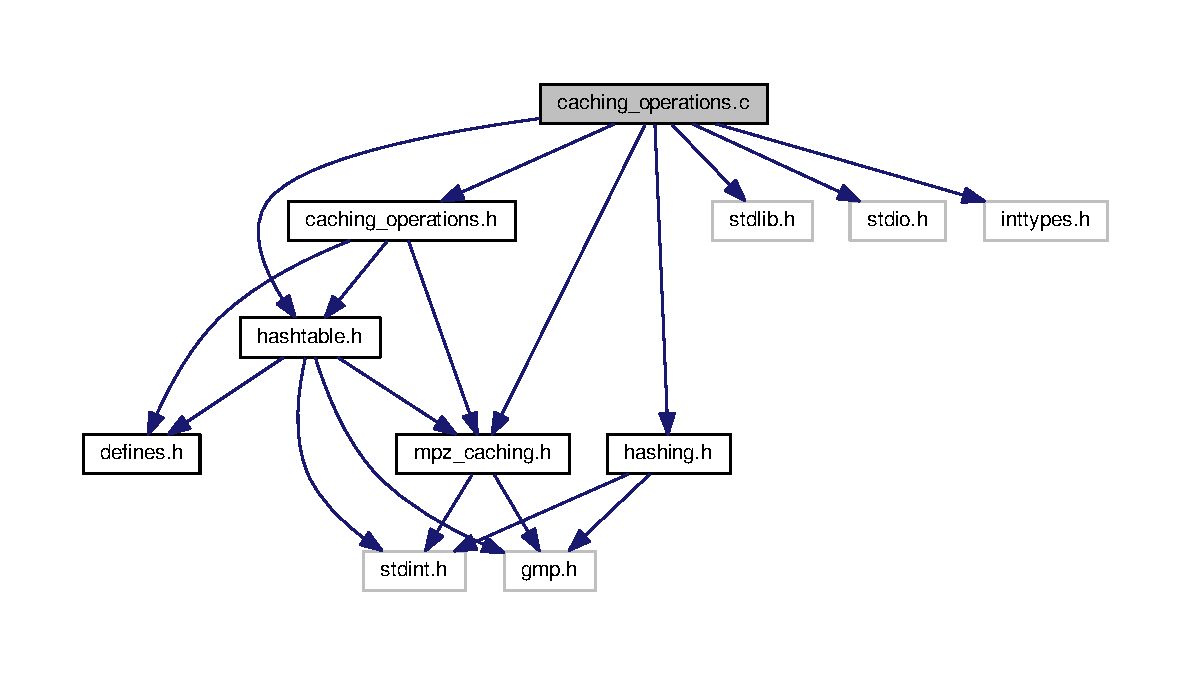
\includegraphics[width=350pt]{caching__operations_8c__incl}
\end{center}
\end{figure}
\subsection*{Functions}
\begin{DoxyCompactItemize}
\item 
uint64\+\_\+t \hyperlink{caching__operations_8c_af24ac6bfb6b961f29854a77b0fd1cdcd}{cache\+\_\+insert\+\_\+mpz\+\_\+raw} (\hyperlink{structlookup}{lookup} $\ast$lu, mpz\+\_\+t val)
\begin{DoxyCompactList}\small\item\em (for internal use only!) cache an mpz\+\_\+t \end{DoxyCompactList}\item 
uint64\+\_\+t \hyperlink{caching__operations_8c_a8378b6353d6fcf409299ae5d043405b2}{cache\+\_\+exists\+\_\+mpz\+\_\+raw} (\hyperlink{structlookup}{lookup} $\ast$lu, mpz\+\_\+t val)
\begin{DoxyCompactList}\small\item\em (for internal use only!) check if an mpz\+\_\+t already exists in cache \end{DoxyCompactList}\item 
uint64\+\_\+t \hyperlink{caching__operations_8c_a086dd00f1d95d3876f60c660c28f4655}{cache\+\_\+exists\+\_\+mpz\+\_\+binary\+\_\+raw} (\hyperlink{structlookup}{lookup} $\ast$cache, mpz\+\_\+t op1, mpz\+\_\+t op2, uint64\+\_\+t $\ast$extra\+\_\+info, int op)
\begin{DoxyCompactList}\small\item\em (for internal use only!) check if a binary operation mpz\+\_\+t x mpz\+\_\+t -\/$>$ mpt\+\_\+t exists \end{DoxyCompactList}\item 
void \hyperlink{caching__operations_8c_a9d0deb4e421d3539ca702e1d25a454bc}{init\+\_\+cache} (\hyperlink{structlookup}{lookup} $\ast$cache, uint64\+\_\+t cachesize)
\begin{DoxyCompactList}\small\item\em initialization of the lookup cache containing the hashtables and the actual cache \end{DoxyCompactList}\item 
void \hyperlink{caching__operations_8c_a5bf3baf9276c8b7f7e04b54a6d50836e}{delete\+\_\+cache} (\hyperlink{structlookup}{lookup} $\ast$cache)
\begin{DoxyCompactList}\small\item\em deletion of the cache and the underlying data structures \end{DoxyCompactList}\item 
void \hyperlink{caching__operations_8c_a14dba9d2bb5513f288c13a42127aa5d8}{get\+\_\+mpz} (\hyperlink{structlookup}{lookup} $\ast$cache, uint64\+\_\+t id, mpz\+\_\+t val)
\begin{DoxyCompactList}\small\item\em function for master cache to set a mpz\+\_\+t and get back an id \end{DoxyCompactList}\item 
double \hyperlink{caching__operations_8c_ab916e2c8a7127d6b8d2daa5723686313}{get\+\_\+double} (\hyperlink{structlookup}{lookup} $\ast$cache, uint64\+\_\+t id)
\begin{DoxyCompactList}\small\item\em function for master cache to set a mpz\+\_\+t and get back an id \end{DoxyCompactList}\item 
uint64\+\_\+t \hyperlink{caching__operations_8c_a5be5a3ac60ee70c550943ca7210ed0ad}{cache\+\_\+insert\+\_\+mpz} (\hyperlink{structlookup}{lookup} $\ast$lu, mpz\+\_\+t val)
\begin{DoxyCompactList}\small\item\em cache an mpz\+\_\+t \end{DoxyCompactList}\item 
uint64\+\_\+t \hyperlink{caching__operations_8c_a56daf76d7d1d61b8c7616dc6b4879cb4}{cache\+\_\+exists\+\_\+mpz} (\hyperlink{structlookup}{lookup} $\ast$lu, mpz\+\_\+t val)
\begin{DoxyCompactList}\small\item\em check if an mpz\+\_\+t already exists in cache \end{DoxyCompactList}\item 
uint64\+\_\+t \hyperlink{caching__operations_8c_a7c5e3db12104bd0cc6a006b02af6d68f}{cache\+\_\+exists\+\_\+mpz\+\_\+binary} (\hyperlink{structlookup}{lookup} $\ast$cache, mpz\+\_\+t op1, mpz\+\_\+t op2, uint64\+\_\+t $\ast$extra\+\_\+info, int op)
\begin{DoxyCompactList}\small\item\em check if a binary operation mpz\+\_\+t x mpz\+\_\+t -\/$>$ mpt\+\_\+t exists \end{DoxyCompactList}\item 
void \hyperlink{caching__operations_8c_a7ea00a65df3156e97a088f4609996b1f}{mpz\+\_\+swap} (mpz\+\_\+t op1, mpz\+\_\+t op2)
\begin{DoxyCompactList}\small\item\em swap two mpz\+\_\+t\textquotesingle{}s \end{DoxyCompactList}\item 
uint64\+\_\+t \hyperlink{caching__operations_8c_aa98a971c3afc7ff1d3ade18670a22042}{cached\+\_\+mpz\+\_\+add} (\hyperlink{structlookup}{lookup} $\ast$cache, mpz\+\_\+t op1\+\_\+in, mpz\+\_\+t op2\+\_\+in)
\begin{DoxyCompactList}\small\item\em addition of two mpz\+\_\+t, the operation and result are cached. \end{DoxyCompactList}\item 
uint64\+\_\+t \hyperlink{caching__operations_8c_ade2fa50c243e70384beb751d1961708a}{cached\+\_\+mpz\+\_\+sub} (\hyperlink{structlookup}{lookup} $\ast$cache, mpz\+\_\+t op1, mpz\+\_\+t op2)
\begin{DoxyCompactList}\small\item\em subtraction of two mpz\+\_\+t, the operation and result are cached. \end{DoxyCompactList}\item 
uint64\+\_\+t \hyperlink{caching__operations_8c_a745a92c531d7f1b4075fdedf31b970c4}{cached\+\_\+mpz\+\_\+mul} (\hyperlink{structlookup}{lookup} $\ast$cache, mpz\+\_\+t op1, mpz\+\_\+t op2)
\begin{DoxyCompactList}\small\item\em multiplication of two mpz\+\_\+t, the operation and result are cached. \end{DoxyCompactList}\item 
uint64\+\_\+t \hyperlink{caching__operations_8c_aa55ef35c74d3f9f270d3899adeaad0da}{cached\+\_\+mpz\+\_\+tdiv} (\hyperlink{structlookup}{lookup} $\ast$cache, uint64\+\_\+t $\ast$rest, mpz\+\_\+t op1, mpz\+\_\+t op2)
\begin{DoxyCompactList}\small\item\em integer division of two mpz\+\_\+t, the operation and result are cached. \end{DoxyCompactList}\item 
uint64\+\_\+t \hyperlink{caching__operations_8c_aeffd662de6699ec5c8f870c70ea8e612}{cached\+\_\+mpz\+\_\+mod} (\hyperlink{structlookup}{lookup} $\ast$cache, mpz\+\_\+t op1, mpz\+\_\+t op2)
\begin{DoxyCompactList}\small\item\em modulo of two mpz\+\_\+t, the operation and result are cached. \end{DoxyCompactList}\item 
uint64\+\_\+t \hyperlink{caching__operations_8c_a8ca5e7ca205dc3b211702f891d5b5f49}{cached\+\_\+mpz\+\_\+gcd} (\hyperlink{structlookup}{lookup} $\ast$cache, mpz\+\_\+t op1, mpz\+\_\+t op2)
\begin{DoxyCompactList}\small\item\em greatest common divisor of two mpz\+\_\+t, the operation and result are cached. \end{DoxyCompactList}\item 
uint64\+\_\+t \hyperlink{caching__operations_8c_a58b9d53218eca4d5c254a4500f621322}{cached\+\_\+mpz\+\_\+invert} (\hyperlink{structlookup}{lookup} $\ast$cache, mpz\+\_\+t op, mpz\+\_\+t mod)
\begin{DoxyCompactList}\small\item\em modular multiplicative inverse of op modulo mod, the operation and result are cached. \end{DoxyCompactList}\end{DoxyCompactItemize}


\subsection{Detailed Description}
caching operations if numbers are large and not directly used 

\begin{DoxyAuthor}{Author}
Sandra Hicks 
\end{DoxyAuthor}


\subsection{Function Documentation}
\index{caching\+\_\+operations.\+c@{caching\+\_\+operations.\+c}!cache\+\_\+exists\+\_\+mpz@{cache\+\_\+exists\+\_\+mpz}}
\index{cache\+\_\+exists\+\_\+mpz@{cache\+\_\+exists\+\_\+mpz}!caching\+\_\+operations.\+c@{caching\+\_\+operations.\+c}}
\subsubsection[{\texorpdfstring{cache\+\_\+exists\+\_\+mpz(lookup $\ast$lu, mpz\+\_\+t val)}{cache_exists_mpz(lookup *lu, mpz_t val)}}]{\setlength{\rightskip}{0pt plus 5cm}uint64\+\_\+t cache\+\_\+exists\+\_\+mpz (
\begin{DoxyParamCaption}
\item[{{\bf lookup} $\ast$}]{lu, }
\item[{mpz\+\_\+t}]{val}
\end{DoxyParamCaption}
)}\hypertarget{caching__operations_8c_a56daf76d7d1d61b8c7616dc6b4879cb4}{}\label{caching__operations_8c_a56daf76d7d1d61b8c7616dc6b4879cb4}


check if an mpz\+\_\+t already exists in cache 


\begin{DoxyParams}{Parameters}
{\em lu} & lookup cache pointer \\
\hline
{\em val} & mpz\+\_\+t which should be checked \\
\hline
\end{DoxyParams}
\begin{DoxyReturn}{Returns}
id for cached mpz\+\_\+t 
\end{DoxyReturn}
\index{caching\+\_\+operations.\+c@{caching\+\_\+operations.\+c}!cache\+\_\+exists\+\_\+mpz\+\_\+binary@{cache\+\_\+exists\+\_\+mpz\+\_\+binary}}
\index{cache\+\_\+exists\+\_\+mpz\+\_\+binary@{cache\+\_\+exists\+\_\+mpz\+\_\+binary}!caching\+\_\+operations.\+c@{caching\+\_\+operations.\+c}}
\subsubsection[{\texorpdfstring{cache\+\_\+exists\+\_\+mpz\+\_\+binary(lookup $\ast$cache, mpz\+\_\+t op1, mpz\+\_\+t op2, uint64\+\_\+t $\ast$extra\+\_\+info, int op)}{cache_exists_mpz_binary(lookup *cache, mpz_t op1, mpz_t op2, uint64_t *extra_info, int op)}}]{\setlength{\rightskip}{0pt plus 5cm}uint64\+\_\+t cache\+\_\+exists\+\_\+mpz\+\_\+binary (
\begin{DoxyParamCaption}
\item[{{\bf lookup} $\ast$}]{cache, }
\item[{mpz\+\_\+t}]{op1, }
\item[{mpz\+\_\+t}]{op2, }
\item[{uint64\+\_\+t $\ast$}]{extra\+\_\+info, }
\item[{int}]{op}
\end{DoxyParamCaption}
)}\hypertarget{caching__operations_8c_a7c5e3db12104bd0cc6a006b02af6d68f}{}\label{caching__operations_8c_a7c5e3db12104bd0cc6a006b02af6d68f}


check if a binary operation mpz\+\_\+t x mpz\+\_\+t -\/$>$ mpt\+\_\+t exists 


\begin{DoxyParams}{Parameters}
{\em cache} & lookup cache pointer \\
\hline
{\em op1} & mpz\+\_\+t first operator \\
\hline
{\em op2} & mpz\+\_\+t second operator \\
\hline
{\em extra\+\_\+info} & pointer for extra information if existent (e.\+g. rest in integer division) \\
\hline
{\em op} & operator which is used \\
\hline
\end{DoxyParams}
\begin{DoxyReturn}{Returns}
id for cached mpz\+\_\+t if existent, 0 if not cached 
\end{DoxyReturn}
\index{caching\+\_\+operations.\+c@{caching\+\_\+operations.\+c}!cache\+\_\+exists\+\_\+mpz\+\_\+binary\+\_\+raw@{cache\+\_\+exists\+\_\+mpz\+\_\+binary\+\_\+raw}}
\index{cache\+\_\+exists\+\_\+mpz\+\_\+binary\+\_\+raw@{cache\+\_\+exists\+\_\+mpz\+\_\+binary\+\_\+raw}!caching\+\_\+operations.\+c@{caching\+\_\+operations.\+c}}
\subsubsection[{\texorpdfstring{cache\+\_\+exists\+\_\+mpz\+\_\+binary\+\_\+raw(lookup $\ast$cache, mpz\+\_\+t op1, mpz\+\_\+t op2, uint64\+\_\+t $\ast$extra\+\_\+info, int op)}{cache_exists_mpz_binary_raw(lookup *cache, mpz_t op1, mpz_t op2, uint64_t *extra_info, int op)}}]{\setlength{\rightskip}{0pt plus 5cm}uint64\+\_\+t cache\+\_\+exists\+\_\+mpz\+\_\+binary\+\_\+raw (
\begin{DoxyParamCaption}
\item[{{\bf lookup} $\ast$}]{cache, }
\item[{mpz\+\_\+t}]{op1, }
\item[{mpz\+\_\+t}]{op2, }
\item[{uint64\+\_\+t $\ast$}]{extra\+\_\+info, }
\item[{int}]{op}
\end{DoxyParamCaption}
)}\hypertarget{caching__operations_8c_a086dd00f1d95d3876f60c660c28f4655}{}\label{caching__operations_8c_a086dd00f1d95d3876f60c660c28f4655}


(for internal use only!) check if a binary operation mpz\+\_\+t x mpz\+\_\+t -\/$>$ mpt\+\_\+t exists 


\begin{DoxyParams}{Parameters}
{\em cache} & lookup cache pointer \\
\hline
{\em op1} & mpz\+\_\+t first operator \\
\hline
{\em op2} & mpz\+\_\+t second operator \\
\hline
{\em extra\+\_\+info} & pointer for extra information if existent (e.\+g. rest in integer division) \\
\hline
{\em op} & operator which is used \\
\hline
\end{DoxyParams}
\begin{DoxyReturn}{Returns}
id for cached mpz\+\_\+t if existent, 0 if not cached 
\end{DoxyReturn}
\index{caching\+\_\+operations.\+c@{caching\+\_\+operations.\+c}!cache\+\_\+exists\+\_\+mpz\+\_\+raw@{cache\+\_\+exists\+\_\+mpz\+\_\+raw}}
\index{cache\+\_\+exists\+\_\+mpz\+\_\+raw@{cache\+\_\+exists\+\_\+mpz\+\_\+raw}!caching\+\_\+operations.\+c@{caching\+\_\+operations.\+c}}
\subsubsection[{\texorpdfstring{cache\+\_\+exists\+\_\+mpz\+\_\+raw(lookup $\ast$lu, mpz\+\_\+t val)}{cache_exists_mpz_raw(lookup *lu, mpz_t val)}}]{\setlength{\rightskip}{0pt plus 5cm}uint64\+\_\+t cache\+\_\+exists\+\_\+mpz\+\_\+raw (
\begin{DoxyParamCaption}
\item[{{\bf lookup} $\ast$}]{lu, }
\item[{mpz\+\_\+t}]{val}
\end{DoxyParamCaption}
)}\hypertarget{caching__operations_8c_a8378b6353d6fcf409299ae5d043405b2}{}\label{caching__operations_8c_a8378b6353d6fcf409299ae5d043405b2}


(for internal use only!) check if an mpz\+\_\+t already exists in cache 


\begin{DoxyParams}{Parameters}
{\em lu} & lookup cache pointer \\
\hline
{\em val} & mpz\+\_\+t which should be checked \\
\hline
\end{DoxyParams}
\begin{DoxyReturn}{Returns}
id for cached mpz\+\_\+t 
\end{DoxyReturn}
\index{caching\+\_\+operations.\+c@{caching\+\_\+operations.\+c}!cache\+\_\+insert\+\_\+mpz@{cache\+\_\+insert\+\_\+mpz}}
\index{cache\+\_\+insert\+\_\+mpz@{cache\+\_\+insert\+\_\+mpz}!caching\+\_\+operations.\+c@{caching\+\_\+operations.\+c}}
\subsubsection[{\texorpdfstring{cache\+\_\+insert\+\_\+mpz(lookup $\ast$lu, mpz\+\_\+t val)}{cache_insert_mpz(lookup *lu, mpz_t val)}}]{\setlength{\rightskip}{0pt plus 5cm}uint64\+\_\+t cache\+\_\+insert\+\_\+mpz (
\begin{DoxyParamCaption}
\item[{{\bf lookup} $\ast$}]{lu, }
\item[{mpz\+\_\+t}]{val}
\end{DoxyParamCaption}
)}\hypertarget{caching__operations_8c_a5be5a3ac60ee70c550943ca7210ed0ad}{}\label{caching__operations_8c_a5be5a3ac60ee70c550943ca7210ed0ad}


cache an mpz\+\_\+t 


\begin{DoxyParams}{Parameters}
{\em lu} & lookup cache pointer \\
\hline
{\em val} & mpz\+\_\+t which should be cached \\
\hline
\end{DoxyParams}
\begin{DoxyReturn}{Returns}
id for cached mpz\+\_\+t 
\end{DoxyReturn}
\index{caching\+\_\+operations.\+c@{caching\+\_\+operations.\+c}!cache\+\_\+insert\+\_\+mpz\+\_\+raw@{cache\+\_\+insert\+\_\+mpz\+\_\+raw}}
\index{cache\+\_\+insert\+\_\+mpz\+\_\+raw@{cache\+\_\+insert\+\_\+mpz\+\_\+raw}!caching\+\_\+operations.\+c@{caching\+\_\+operations.\+c}}
\subsubsection[{\texorpdfstring{cache\+\_\+insert\+\_\+mpz\+\_\+raw(lookup $\ast$lu, mpz\+\_\+t val)}{cache_insert_mpz_raw(lookup *lu, mpz_t val)}}]{\setlength{\rightskip}{0pt plus 5cm}uint64\+\_\+t cache\+\_\+insert\+\_\+mpz\+\_\+raw (
\begin{DoxyParamCaption}
\item[{{\bf lookup} $\ast$}]{lu, }
\item[{mpz\+\_\+t}]{val}
\end{DoxyParamCaption}
)}\hypertarget{caching__operations_8c_af24ac6bfb6b961f29854a77b0fd1cdcd}{}\label{caching__operations_8c_af24ac6bfb6b961f29854a77b0fd1cdcd}


(for internal use only!) cache an mpz\+\_\+t 


\begin{DoxyParams}{Parameters}
{\em lu} & lookup cache pointer \\
\hline
{\em val} & mpz\+\_\+t which should be cached \\
\hline
\end{DoxyParams}
\begin{DoxyReturn}{Returns}
id for cached mpz\+\_\+t 
\end{DoxyReturn}
\index{caching\+\_\+operations.\+c@{caching\+\_\+operations.\+c}!cached\+\_\+mpz\+\_\+add@{cached\+\_\+mpz\+\_\+add}}
\index{cached\+\_\+mpz\+\_\+add@{cached\+\_\+mpz\+\_\+add}!caching\+\_\+operations.\+c@{caching\+\_\+operations.\+c}}
\subsubsection[{\texorpdfstring{cached\+\_\+mpz\+\_\+add(lookup $\ast$cache, mpz\+\_\+t op1\+\_\+in, mpz\+\_\+t op2\+\_\+in)}{cached_mpz_add(lookup *cache, mpz_t op1_in, mpz_t op2_in)}}]{\setlength{\rightskip}{0pt plus 5cm}uint64\+\_\+t cached\+\_\+mpz\+\_\+add (
\begin{DoxyParamCaption}
\item[{{\bf lookup} $\ast$}]{cache, }
\item[{mpz\+\_\+t}]{op1\+\_\+in, }
\item[{mpz\+\_\+t}]{op2\+\_\+in}
\end{DoxyParamCaption}
)}\hypertarget{caching__operations_8c_aa98a971c3afc7ff1d3ade18670a22042}{}\label{caching__operations_8c_aa98a971c3afc7ff1d3ade18670a22042}


addition of two mpz\+\_\+t, the operation and result are cached. 


\begin{DoxyParams}{Parameters}
{\em cache} & lookup cache pointer \\
\hline
{\em op1\+\_\+in} & first operand \\
\hline
{\em op2\+\_\+in} & second operand \\
\hline
\end{DoxyParams}
\begin{DoxyReturn}{Returns}
id to result of addition 
\end{DoxyReturn}
\index{caching\+\_\+operations.\+c@{caching\+\_\+operations.\+c}!cached\+\_\+mpz\+\_\+gcd@{cached\+\_\+mpz\+\_\+gcd}}
\index{cached\+\_\+mpz\+\_\+gcd@{cached\+\_\+mpz\+\_\+gcd}!caching\+\_\+operations.\+c@{caching\+\_\+operations.\+c}}
\subsubsection[{\texorpdfstring{cached\+\_\+mpz\+\_\+gcd(lookup $\ast$cache, mpz\+\_\+t op1, mpz\+\_\+t op2)}{cached_mpz_gcd(lookup *cache, mpz_t op1, mpz_t op2)}}]{\setlength{\rightskip}{0pt plus 5cm}uint64\+\_\+t cached\+\_\+mpz\+\_\+gcd (
\begin{DoxyParamCaption}
\item[{{\bf lookup} $\ast$}]{cache, }
\item[{mpz\+\_\+t}]{op1, }
\item[{mpz\+\_\+t}]{op2}
\end{DoxyParamCaption}
)}\hypertarget{caching__operations_8c_a8ca5e7ca205dc3b211702f891d5b5f49}{}\label{caching__operations_8c_a8ca5e7ca205dc3b211702f891d5b5f49}


greatest common divisor of two mpz\+\_\+t, the operation and result are cached. 


\begin{DoxyParams}{Parameters}
{\em cache} & lookup cache pointer \\
\hline
{\em op1} & first operand \\
\hline
{\em op2} & second operand \\
\hline
\end{DoxyParams}
\begin{DoxyReturn}{Returns}
id to result of greatest common divisor 
\end{DoxyReturn}
\index{caching\+\_\+operations.\+c@{caching\+\_\+operations.\+c}!cached\+\_\+mpz\+\_\+invert@{cached\+\_\+mpz\+\_\+invert}}
\index{cached\+\_\+mpz\+\_\+invert@{cached\+\_\+mpz\+\_\+invert}!caching\+\_\+operations.\+c@{caching\+\_\+operations.\+c}}
\subsubsection[{\texorpdfstring{cached\+\_\+mpz\+\_\+invert(lookup $\ast$cache, mpz\+\_\+t op, mpz\+\_\+t mod)}{cached_mpz_invert(lookup *cache, mpz_t op, mpz_t mod)}}]{\setlength{\rightskip}{0pt plus 5cm}uint64\+\_\+t cached\+\_\+mpz\+\_\+invert (
\begin{DoxyParamCaption}
\item[{{\bf lookup} $\ast$}]{cache, }
\item[{mpz\+\_\+t}]{op, }
\item[{mpz\+\_\+t}]{mod}
\end{DoxyParamCaption}
)}\hypertarget{caching__operations_8c_a58b9d53218eca4d5c254a4500f621322}{}\label{caching__operations_8c_a58b9d53218eca4d5c254a4500f621322}


modular multiplicative inverse of op modulo mod, the operation and result are cached. 


\begin{DoxyParams}{Parameters}
{\em cache} & lookup cache pointer \\
\hline
{\em op} & first operand \\
\hline
{\em mod} & second operand \\
\hline
\end{DoxyParams}
\begin{DoxyReturn}{Returns}
id to result of inverse, 0 if non existent 
\end{DoxyReturn}
\index{caching\+\_\+operations.\+c@{caching\+\_\+operations.\+c}!cached\+\_\+mpz\+\_\+mod@{cached\+\_\+mpz\+\_\+mod}}
\index{cached\+\_\+mpz\+\_\+mod@{cached\+\_\+mpz\+\_\+mod}!caching\+\_\+operations.\+c@{caching\+\_\+operations.\+c}}
\subsubsection[{\texorpdfstring{cached\+\_\+mpz\+\_\+mod(lookup $\ast$cache, mpz\+\_\+t op1, mpz\+\_\+t op2)}{cached_mpz_mod(lookup *cache, mpz_t op1, mpz_t op2)}}]{\setlength{\rightskip}{0pt plus 5cm}uint64\+\_\+t cached\+\_\+mpz\+\_\+mod (
\begin{DoxyParamCaption}
\item[{{\bf lookup} $\ast$}]{cache, }
\item[{mpz\+\_\+t}]{op1, }
\item[{mpz\+\_\+t}]{op2}
\end{DoxyParamCaption}
)}\hypertarget{caching__operations_8c_aeffd662de6699ec5c8f870c70ea8e612}{}\label{caching__operations_8c_aeffd662de6699ec5c8f870c70ea8e612}


modulo of two mpz\+\_\+t, the operation and result are cached. 


\begin{DoxyParams}{Parameters}
{\em cache} & lookup cache pointer \\
\hline
{\em op1} & first operand \\
\hline
{\em op2} & second operand \\
\hline
\end{DoxyParams}
\begin{DoxyReturn}{Returns}
id to result of modulo operation 
\end{DoxyReturn}
\index{caching\+\_\+operations.\+c@{caching\+\_\+operations.\+c}!cached\+\_\+mpz\+\_\+mul@{cached\+\_\+mpz\+\_\+mul}}
\index{cached\+\_\+mpz\+\_\+mul@{cached\+\_\+mpz\+\_\+mul}!caching\+\_\+operations.\+c@{caching\+\_\+operations.\+c}}
\subsubsection[{\texorpdfstring{cached\+\_\+mpz\+\_\+mul(lookup $\ast$cache, mpz\+\_\+t op1, mpz\+\_\+t op2)}{cached_mpz_mul(lookup *cache, mpz_t op1, mpz_t op2)}}]{\setlength{\rightskip}{0pt plus 5cm}uint64\+\_\+t cached\+\_\+mpz\+\_\+mul (
\begin{DoxyParamCaption}
\item[{{\bf lookup} $\ast$}]{cache, }
\item[{mpz\+\_\+t}]{op1, }
\item[{mpz\+\_\+t}]{op2}
\end{DoxyParamCaption}
)}\hypertarget{caching__operations_8c_a745a92c531d7f1b4075fdedf31b970c4}{}\label{caching__operations_8c_a745a92c531d7f1b4075fdedf31b970c4}


multiplication of two mpz\+\_\+t, the operation and result are cached. 


\begin{DoxyParams}{Parameters}
{\em cache} & lookup cache pointer \\
\hline
{\em op1} & first operand \\
\hline
{\em op2} & second operand \\
\hline
\end{DoxyParams}
\begin{DoxyReturn}{Returns}
id to result of multiplication 
\end{DoxyReturn}
\index{caching\+\_\+operations.\+c@{caching\+\_\+operations.\+c}!cached\+\_\+mpz\+\_\+sub@{cached\+\_\+mpz\+\_\+sub}}
\index{cached\+\_\+mpz\+\_\+sub@{cached\+\_\+mpz\+\_\+sub}!caching\+\_\+operations.\+c@{caching\+\_\+operations.\+c}}
\subsubsection[{\texorpdfstring{cached\+\_\+mpz\+\_\+sub(lookup $\ast$cache, mpz\+\_\+t op1, mpz\+\_\+t op2)}{cached_mpz_sub(lookup *cache, mpz_t op1, mpz_t op2)}}]{\setlength{\rightskip}{0pt plus 5cm}uint64\+\_\+t cached\+\_\+mpz\+\_\+sub (
\begin{DoxyParamCaption}
\item[{{\bf lookup} $\ast$}]{cache, }
\item[{mpz\+\_\+t}]{op1, }
\item[{mpz\+\_\+t}]{op2}
\end{DoxyParamCaption}
)}\hypertarget{caching__operations_8c_ade2fa50c243e70384beb751d1961708a}{}\label{caching__operations_8c_ade2fa50c243e70384beb751d1961708a}


subtraction of two mpz\+\_\+t, the operation and result are cached. 


\begin{DoxyParams}{Parameters}
{\em cache} & lookup cache pointer \\
\hline
{\em op1} & first operand \\
\hline
{\em op2} & second operand \\
\hline
\end{DoxyParams}
\begin{DoxyReturn}{Returns}
id to result of subtraction 
\end{DoxyReturn}
\index{caching\+\_\+operations.\+c@{caching\+\_\+operations.\+c}!cached\+\_\+mpz\+\_\+tdiv@{cached\+\_\+mpz\+\_\+tdiv}}
\index{cached\+\_\+mpz\+\_\+tdiv@{cached\+\_\+mpz\+\_\+tdiv}!caching\+\_\+operations.\+c@{caching\+\_\+operations.\+c}}
\subsubsection[{\texorpdfstring{cached\+\_\+mpz\+\_\+tdiv(lookup $\ast$cache, uint64\+\_\+t $\ast$rest, mpz\+\_\+t op1, mpz\+\_\+t op2)}{cached_mpz_tdiv(lookup *cache, uint64_t *rest, mpz_t op1, mpz_t op2)}}]{\setlength{\rightskip}{0pt plus 5cm}uint64\+\_\+t cached\+\_\+mpz\+\_\+tdiv (
\begin{DoxyParamCaption}
\item[{{\bf lookup} $\ast$}]{cache, }
\item[{uint64\+\_\+t $\ast$}]{rest, }
\item[{mpz\+\_\+t}]{op1, }
\item[{mpz\+\_\+t}]{op2}
\end{DoxyParamCaption}
)}\hypertarget{caching__operations_8c_aa55ef35c74d3f9f270d3899adeaad0da}{}\label{caching__operations_8c_aa55ef35c74d3f9f270d3899adeaad0da}


integer division of two mpz\+\_\+t, the operation and result are cached. 


\begin{DoxyParams}{Parameters}
{\em cache} & lookup cache pointer \\
\hline
{\em rest} & pointer to store the rest of the integer division \\
\hline
{\em op1} & first operand \\
\hline
{\em op2} & second operand \\
\hline
\end{DoxyParams}
\begin{DoxyReturn}{Returns}
id to result of division 
\end{DoxyReturn}
\index{caching\+\_\+operations.\+c@{caching\+\_\+operations.\+c}!delete\+\_\+cache@{delete\+\_\+cache}}
\index{delete\+\_\+cache@{delete\+\_\+cache}!caching\+\_\+operations.\+c@{caching\+\_\+operations.\+c}}
\subsubsection[{\texorpdfstring{delete\+\_\+cache(lookup $\ast$cache)}{delete_cache(lookup *cache)}}]{\setlength{\rightskip}{0pt plus 5cm}void delete\+\_\+cache (
\begin{DoxyParamCaption}
\item[{{\bf lookup} $\ast$}]{cache}
\end{DoxyParamCaption}
)}\hypertarget{caching__operations_8c_a5bf3baf9276c8b7f7e04b54a6d50836e}{}\label{caching__operations_8c_a5bf3baf9276c8b7f7e04b54a6d50836e}


deletion of the cache and the underlying data structures 


\begin{DoxyParams}{Parameters}
{\em cache} & lookup cache pointer \\
\hline
\end{DoxyParams}
\index{caching\+\_\+operations.\+c@{caching\+\_\+operations.\+c}!get\+\_\+double@{get\+\_\+double}}
\index{get\+\_\+double@{get\+\_\+double}!caching\+\_\+operations.\+c@{caching\+\_\+operations.\+c}}
\subsubsection[{\texorpdfstring{get\+\_\+double(lookup $\ast$cache, uint64\+\_\+t id)}{get_double(lookup *cache, uint64_t id)}}]{\setlength{\rightskip}{0pt plus 5cm}double get\+\_\+double (
\begin{DoxyParamCaption}
\item[{{\bf lookup} $\ast$}]{cache, }
\item[{uint64\+\_\+t}]{id}
\end{DoxyParamCaption}
)}\hypertarget{caching__operations_8c_ab916e2c8a7127d6b8d2daa5723686313}{}\label{caching__operations_8c_ab916e2c8a7127d6b8d2daa5723686313}


function for master cache to set a mpz\+\_\+t and get back an id 


\begin{DoxyParams}{Parameters}
{\em cache} & lookup cache pointer \\
\hline
{\em id} & for cached mpz\+\_\+t \\
\hline
\end{DoxyParams}
\begin{DoxyReturn}{Returns}
double representation for mpz\+\_\+t 
\end{DoxyReturn}
\index{caching\+\_\+operations.\+c@{caching\+\_\+operations.\+c}!get\+\_\+mpz@{get\+\_\+mpz}}
\index{get\+\_\+mpz@{get\+\_\+mpz}!caching\+\_\+operations.\+c@{caching\+\_\+operations.\+c}}
\subsubsection[{\texorpdfstring{get\+\_\+mpz(lookup $\ast$cache, uint64\+\_\+t id, mpz\+\_\+t val)}{get_mpz(lookup *cache, uint64_t id, mpz_t val)}}]{\setlength{\rightskip}{0pt plus 5cm}void get\+\_\+mpz (
\begin{DoxyParamCaption}
\item[{{\bf lookup} $\ast$}]{cache, }
\item[{uint64\+\_\+t}]{id, }
\item[{mpz\+\_\+t}]{val}
\end{DoxyParamCaption}
)}\hypertarget{caching__operations_8c_a14dba9d2bb5513f288c13a42127aa5d8}{}\label{caching__operations_8c_a14dba9d2bb5513f288c13a42127aa5d8}


function for master cache to set a mpz\+\_\+t and get back an id 


\begin{DoxyParams}{Parameters}
{\em cache} & lookup cache pointer \\
\hline
{\em id} & id for cached mpz\+\_\+t \\
\hline
{\em val} & for writing the result \\
\hline
\end{DoxyParams}
\index{caching\+\_\+operations.\+c@{caching\+\_\+operations.\+c}!init\+\_\+cache@{init\+\_\+cache}}
\index{init\+\_\+cache@{init\+\_\+cache}!caching\+\_\+operations.\+c@{caching\+\_\+operations.\+c}}
\subsubsection[{\texorpdfstring{init\+\_\+cache(lookup $\ast$cache, uint64\+\_\+t cachesize)}{init_cache(lookup *cache, uint64_t cachesize)}}]{\setlength{\rightskip}{0pt plus 5cm}void init\+\_\+cache (
\begin{DoxyParamCaption}
\item[{{\bf lookup} $\ast$}]{cache, }
\item[{uint64\+\_\+t}]{cachesize}
\end{DoxyParamCaption}
)}\hypertarget{caching__operations_8c_a9d0deb4e421d3539ca702e1d25a454bc}{}\label{caching__operations_8c_a9d0deb4e421d3539ca702e1d25a454bc}


initialization of the lookup cache containing the hashtables and the actual cache 


\begin{DoxyParams}{Parameters}
{\em cache} & lookup cache pointer \\
\hline
{\em cachesize} & size of the cache \\
\hline
\end{DoxyParams}
\index{caching\+\_\+operations.\+c@{caching\+\_\+operations.\+c}!mpz\+\_\+swap@{mpz\+\_\+swap}}
\index{mpz\+\_\+swap@{mpz\+\_\+swap}!caching\+\_\+operations.\+c@{caching\+\_\+operations.\+c}}
\subsubsection[{\texorpdfstring{mpz\+\_\+swap(mpz\+\_\+t op1, mpz\+\_\+t op2)}{mpz_swap(mpz_t op1, mpz_t op2)}}]{\setlength{\rightskip}{0pt plus 5cm}void mpz\+\_\+swap (
\begin{DoxyParamCaption}
\item[{mpz\+\_\+t}]{op1, }
\item[{mpz\+\_\+t}]{op2}
\end{DoxyParamCaption}
)}\hypertarget{caching__operations_8c_a7ea00a65df3156e97a088f4609996b1f}{}\label{caching__operations_8c_a7ea00a65df3156e97a088f4609996b1f}


swap two mpz\+\_\+t\textquotesingle{}s 


\begin{DoxyParams}{Parameters}
{\em op1} & \\
\hline
{\em op2} & \\
\hline
\end{DoxyParams}

\hypertarget{caching__operations_8h}{}\section{caching\+\_\+operations.\+h File Reference}
\label{caching__operations_8h}\index{caching\+\_\+operations.\+h@{caching\+\_\+operations.\+h}}


header for caching operations if numbers are large and not directly used  


{\ttfamily \#include \char`\"{}hashtable.\+h\char`\"{}}\\*
{\ttfamily \#include \char`\"{}mpz\+\_\+caching.\+h\char`\"{}}\\*
{\ttfamily \#include \char`\"{}defines.\+h\char`\"{}}\\*
Include dependency graph for caching\+\_\+operations.\+h\+:\nopagebreak
\begin{figure}[H]
\begin{center}
\leavevmode
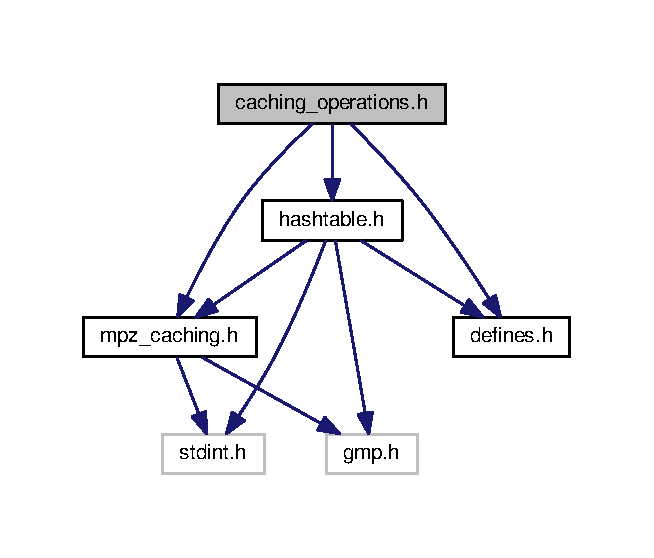
\includegraphics[width=314pt]{caching__operations_8h__incl}
\end{center}
\end{figure}
This graph shows which files directly or indirectly include this file\+:\nopagebreak
\begin{figure}[H]
\begin{center}
\leavevmode
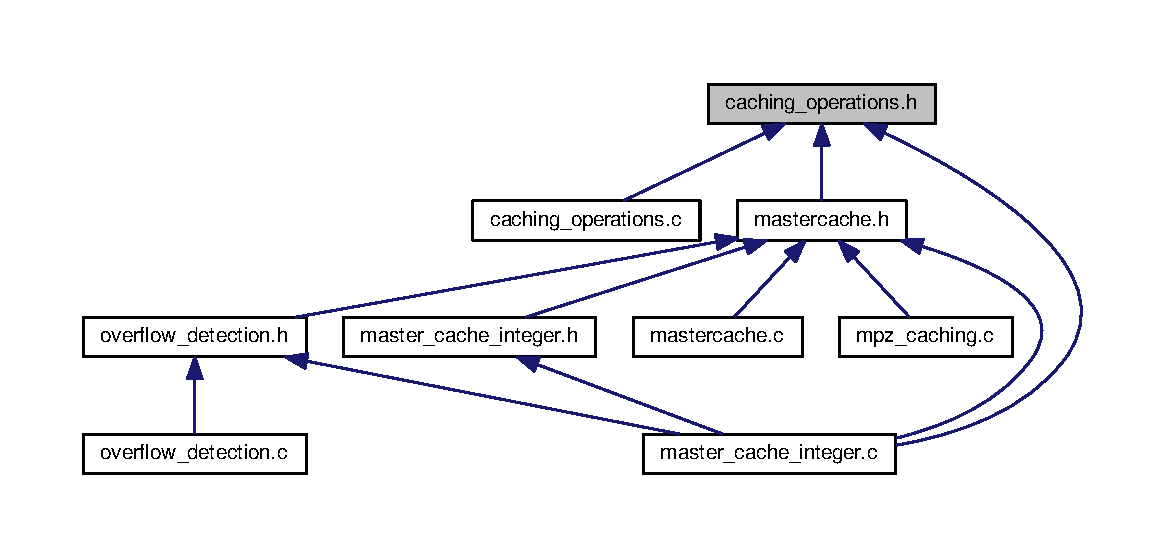
\includegraphics[width=350pt]{caching__operations_8h__dep__incl}
\end{center}
\end{figure}
\subsection*{Classes}
\begin{DoxyCompactItemize}
\item 
struct \hyperlink{structlookup__table}{lookup\+\_\+table}
\begin{DoxyCompactList}\small\item\em lookup table for mpz\+\_\+t \end{DoxyCompactList}\item 
struct \hyperlink{structlookup__table__binary}{lookup\+\_\+table\+\_\+binary}
\begin{DoxyCompactList}\small\item\em lookup table for binary operations mpz\+\_\+t x mpz\+\_\+t -\/$>$ mpz\+\_\+t \end{DoxyCompactList}\item 
struct \hyperlink{structlookup}{lookup}
\begin{DoxyCompactList}\small\item\em collection of lookup tables for the required operations \end{DoxyCompactList}\end{DoxyCompactItemize}
\subsection*{Typedefs}
\begin{DoxyCompactItemize}
\item 
typedef struct \hyperlink{structlookup__table}{lookup\+\_\+table} \hyperlink{caching__operations_8h_a5f315994a3f6986c94c1cf8c1feea2fb}{lookup\+\_\+table}\hypertarget{caching__operations_8h_a5f315994a3f6986c94c1cf8c1feea2fb}{}\label{caching__operations_8h_a5f315994a3f6986c94c1cf8c1feea2fb}

\begin{DoxyCompactList}\small\item\em lookup table for mpz\+\_\+t \end{DoxyCompactList}\item 
typedef struct \hyperlink{structlookup__table__binary}{lookup\+\_\+table\+\_\+binary} \hyperlink{caching__operations_8h_a10378a824d9fad74088e8b761bd88bd0}{lookup\+\_\+table\+\_\+binary}\hypertarget{caching__operations_8h_a10378a824d9fad74088e8b761bd88bd0}{}\label{caching__operations_8h_a10378a824d9fad74088e8b761bd88bd0}

\begin{DoxyCompactList}\small\item\em lookup table for binary operations mpz\+\_\+t x mpz\+\_\+t -\/$>$ mpz\+\_\+t \end{DoxyCompactList}\item 
typedef struct \hyperlink{structlookup}{lookup} \hyperlink{caching__operations_8h_a54725a138fee887b27397d25e09db5d4}{lookup}\hypertarget{caching__operations_8h_a54725a138fee887b27397d25e09db5d4}{}\label{caching__operations_8h_a54725a138fee887b27397d25e09db5d4}

\begin{DoxyCompactList}\small\item\em collection of lookup tables for the required operations \end{DoxyCompactList}\end{DoxyCompactItemize}
\subsection*{Enumerations}
\begin{DoxyCompactItemize}
\item 
enum \hyperlink{caching__operations_8h_aa8f137f19095e0bdcf4f521e901f88bb}{Operation} \{ \\*
\hyperlink{caching__operations_8h_aa8f137f19095e0bdcf4f521e901f88bbacfcf145f2788bf340ff3f3098bc54909}{A\+DD}, 
\hyperlink{caching__operations_8h_aa8f137f19095e0bdcf4f521e901f88bba12b733d4941495e86811fe6ceeeff9da}{S\+UB}, 
\hyperlink{caching__operations_8h_aa8f137f19095e0bdcf4f521e901f88bba086ab1f2f4dac104b6826ebe0eaba8fd}{M\+UL}, 
\hyperlink{caching__operations_8h_aa8f137f19095e0bdcf4f521e901f88bbac3e4cf6bb26322af5dcabd9a3e536863}{T\+D\+IV}, 
\\*
\hyperlink{caching__operations_8h_aa8f137f19095e0bdcf4f521e901f88bba140fcc89db148e5975f1486e794675ba}{M\+OD}, 
\hyperlink{caching__operations_8h_aa8f137f19095e0bdcf4f521e901f88bba1e01e015db0e95c2da032bb76f5ddcc1}{G\+CD}, 
\hyperlink{caching__operations_8h_aa8f137f19095e0bdcf4f521e901f88bba003b741848d7128e25831a8376672700}{I\+NV}
 \}
\end{DoxyCompactItemize}
\subsection*{Functions}
\begin{DoxyCompactItemize}
\item 
void \hyperlink{caching__operations_8h_a9d0deb4e421d3539ca702e1d25a454bc}{init\+\_\+cache} (\hyperlink{structlookup}{lookup} $\ast$cache, uint64\+\_\+t cachesize)
\begin{DoxyCompactList}\small\item\em initialization of the lookup cache containing the hashtables and the actual cache \end{DoxyCompactList}\item 
void \hyperlink{caching__operations_8h_a5bf3baf9276c8b7f7e04b54a6d50836e}{delete\+\_\+cache} (\hyperlink{structlookup}{lookup} $\ast$cache)
\begin{DoxyCompactList}\small\item\em deletion of the cache and the underlying data structures \end{DoxyCompactList}\item 
void \hyperlink{caching__operations_8h_a14dba9d2bb5513f288c13a42127aa5d8}{get\+\_\+mpz} (\hyperlink{structlookup}{lookup} $\ast$cache, uint64\+\_\+t id, mpz\+\_\+t val)
\begin{DoxyCompactList}\small\item\em function for master cache to set a mpz\+\_\+t and get back an id \end{DoxyCompactList}\item 
double \hyperlink{caching__operations_8h_ab916e2c8a7127d6b8d2daa5723686313}{get\+\_\+double} (\hyperlink{structlookup}{lookup} $\ast$cache, uint64\+\_\+t id)
\begin{DoxyCompactList}\small\item\em function for master cache to set a mpz\+\_\+t and get back an id \end{DoxyCompactList}\item 
uint64\+\_\+t \hyperlink{caching__operations_8h_a5be5a3ac60ee70c550943ca7210ed0ad}{cache\+\_\+insert\+\_\+mpz} (\hyperlink{structlookup}{lookup} $\ast$lu, mpz\+\_\+t val)
\begin{DoxyCompactList}\small\item\em cache an mpz\+\_\+t \end{DoxyCompactList}\item 
uint64\+\_\+t \hyperlink{caching__operations_8h_a56daf76d7d1d61b8c7616dc6b4879cb4}{cache\+\_\+exists\+\_\+mpz} (\hyperlink{structlookup}{lookup} $\ast$lu, mpz\+\_\+t val)
\begin{DoxyCompactList}\small\item\em check if an mpz\+\_\+t already exists in cache \end{DoxyCompactList}\item 
uint64\+\_\+t \hyperlink{caching__operations_8h_a7c5e3db12104bd0cc6a006b02af6d68f}{cache\+\_\+exists\+\_\+mpz\+\_\+binary} (\hyperlink{structlookup}{lookup} $\ast$cache, mpz\+\_\+t op1, mpz\+\_\+t op2, uint64\+\_\+t $\ast$extra\+\_\+info, int op)
\begin{DoxyCompactList}\small\item\em check if a binary operation mpz\+\_\+t x mpz\+\_\+t -\/$>$ mpt\+\_\+t exists \end{DoxyCompactList}\item 
uint64\+\_\+t \hyperlink{caching__operations_8h_aa98a971c3afc7ff1d3ade18670a22042}{cached\+\_\+mpz\+\_\+add} (\hyperlink{structlookup}{lookup} $\ast$cache, mpz\+\_\+t op1\+\_\+in, mpz\+\_\+t op2\+\_\+in)
\begin{DoxyCompactList}\small\item\em addition of two mpz\+\_\+t, the operation and result are cached. \end{DoxyCompactList}\item 
uint64\+\_\+t \hyperlink{caching__operations_8h_ade2fa50c243e70384beb751d1961708a}{cached\+\_\+mpz\+\_\+sub} (\hyperlink{structlookup}{lookup} $\ast$cache, mpz\+\_\+t op1, mpz\+\_\+t op2)
\begin{DoxyCompactList}\small\item\em subtraction of two mpz\+\_\+t, the operation and result are cached. \end{DoxyCompactList}\item 
uint64\+\_\+t \hyperlink{caching__operations_8h_a745a92c531d7f1b4075fdedf31b970c4}{cached\+\_\+mpz\+\_\+mul} (\hyperlink{structlookup}{lookup} $\ast$cache, mpz\+\_\+t op1, mpz\+\_\+t op2)
\begin{DoxyCompactList}\small\item\em multiplication of two mpz\+\_\+t, the operation and result are cached. \end{DoxyCompactList}\item 
uint64\+\_\+t \hyperlink{caching__operations_8h_aa55ef35c74d3f9f270d3899adeaad0da}{cached\+\_\+mpz\+\_\+tdiv} (\hyperlink{structlookup}{lookup} $\ast$cache, uint64\+\_\+t $\ast$rest, mpz\+\_\+t op1, mpz\+\_\+t op2)
\begin{DoxyCompactList}\small\item\em integer division of two mpz\+\_\+t, the operation and result are cached. \end{DoxyCompactList}\item 
uint64\+\_\+t \hyperlink{caching__operations_8h_af76568c03fb8ccd12ff15ab71c99c6bd}{cached\+\_\+mpz\+\_\+mod} (\hyperlink{structlookup}{lookup} $\ast$cache, mpz\+\_\+t op, mpz\+\_\+t mod)
\begin{DoxyCompactList}\small\item\em modulo of two mpz\+\_\+t, the operation and result are cached. \end{DoxyCompactList}\item 
uint64\+\_\+t \hyperlink{caching__operations_8h_a8ca5e7ca205dc3b211702f891d5b5f49}{cached\+\_\+mpz\+\_\+gcd} (\hyperlink{structlookup}{lookup} $\ast$cache, mpz\+\_\+t op1, mpz\+\_\+t op2)
\begin{DoxyCompactList}\small\item\em greatest common divisor of two mpz\+\_\+t, the operation and result are cached. \end{DoxyCompactList}\item 
uint64\+\_\+t \hyperlink{caching__operations_8h_a58b9d53218eca4d5c254a4500f621322}{cached\+\_\+mpz\+\_\+invert} (\hyperlink{structlookup}{lookup} $\ast$cache, mpz\+\_\+t op, mpz\+\_\+t mod)
\begin{DoxyCompactList}\small\item\em modular multiplicative inverse of op modulo mod, the operation and result are cached. \end{DoxyCompactList}\end{DoxyCompactItemize}


\subsection{Detailed Description}
header for caching operations if numbers are large and not directly used 

\begin{DoxyAuthor}{Author}
Sandra Hicks 
\end{DoxyAuthor}


\subsection{Enumeration Type Documentation}
\index{caching\+\_\+operations.\+h@{caching\+\_\+operations.\+h}!Operation@{Operation}}
\index{Operation@{Operation}!caching\+\_\+operations.\+h@{caching\+\_\+operations.\+h}}
\subsubsection[{\texorpdfstring{Operation}{Operation}}]{\setlength{\rightskip}{0pt plus 5cm}enum {\bf Operation}}\hypertarget{caching__operations_8h_aa8f137f19095e0bdcf4f521e901f88bb}{}\label{caching__operations_8h_aa8f137f19095e0bdcf4f521e901f88bb}
identifiers for operations applied to mpz\+\_\+t\textquotesingle{}s \begin{Desc}
\item[Enumerator]\par
\begin{description}
\index{A\+DD@{A\+DD}!caching\+\_\+operations.\+h@{caching\+\_\+operations.\+h}}\index{caching\+\_\+operations.\+h@{caching\+\_\+operations.\+h}!A\+DD@{A\+DD}}\item[{\em 
A\+DD\hypertarget{caching__operations_8h_aa8f137f19095e0bdcf4f521e901f88bbacfcf145f2788bf340ff3f3098bc54909}{}\label{caching__operations_8h_aa8f137f19095e0bdcf4f521e901f88bbacfcf145f2788bf340ff3f3098bc54909}
}]addition \index{S\+UB@{S\+UB}!caching\+\_\+operations.\+h@{caching\+\_\+operations.\+h}}\index{caching\+\_\+operations.\+h@{caching\+\_\+operations.\+h}!S\+UB@{S\+UB}}\item[{\em 
S\+UB\hypertarget{caching__operations_8h_aa8f137f19095e0bdcf4f521e901f88bba12b733d4941495e86811fe6ceeeff9da}{}\label{caching__operations_8h_aa8f137f19095e0bdcf4f521e901f88bba12b733d4941495e86811fe6ceeeff9da}
}]subtraction \index{M\+UL@{M\+UL}!caching\+\_\+operations.\+h@{caching\+\_\+operations.\+h}}\index{caching\+\_\+operations.\+h@{caching\+\_\+operations.\+h}!M\+UL@{M\+UL}}\item[{\em 
M\+UL\hypertarget{caching__operations_8h_aa8f137f19095e0bdcf4f521e901f88bba086ab1f2f4dac104b6826ebe0eaba8fd}{}\label{caching__operations_8h_aa8f137f19095e0bdcf4f521e901f88bba086ab1f2f4dac104b6826ebe0eaba8fd}
}]multiplication \index{T\+D\+IV@{T\+D\+IV}!caching\+\_\+operations.\+h@{caching\+\_\+operations.\+h}}\index{caching\+\_\+operations.\+h@{caching\+\_\+operations.\+h}!T\+D\+IV@{T\+D\+IV}}\item[{\em 
T\+D\+IV\hypertarget{caching__operations_8h_aa8f137f19095e0bdcf4f521e901f88bbac3e4cf6bb26322af5dcabd9a3e536863}{}\label{caching__operations_8h_aa8f137f19095e0bdcf4f521e901f88bbac3e4cf6bb26322af5dcabd9a3e536863}
}]integer division \index{M\+OD@{M\+OD}!caching\+\_\+operations.\+h@{caching\+\_\+operations.\+h}}\index{caching\+\_\+operations.\+h@{caching\+\_\+operations.\+h}!M\+OD@{M\+OD}}\item[{\em 
M\+OD\hypertarget{caching__operations_8h_aa8f137f19095e0bdcf4f521e901f88bba140fcc89db148e5975f1486e794675ba}{}\label{caching__operations_8h_aa8f137f19095e0bdcf4f521e901f88bba140fcc89db148e5975f1486e794675ba}
}]modulo \index{G\+CD@{G\+CD}!caching\+\_\+operations.\+h@{caching\+\_\+operations.\+h}}\index{caching\+\_\+operations.\+h@{caching\+\_\+operations.\+h}!G\+CD@{G\+CD}}\item[{\em 
G\+CD\hypertarget{caching__operations_8h_aa8f137f19095e0bdcf4f521e901f88bba1e01e015db0e95c2da032bb76f5ddcc1}{}\label{caching__operations_8h_aa8f137f19095e0bdcf4f521e901f88bba1e01e015db0e95c2da032bb76f5ddcc1}
}]greatest common divisor \index{I\+NV@{I\+NV}!caching\+\_\+operations.\+h@{caching\+\_\+operations.\+h}}\index{caching\+\_\+operations.\+h@{caching\+\_\+operations.\+h}!I\+NV@{I\+NV}}\item[{\em 
I\+NV\hypertarget{caching__operations_8h_aa8f137f19095e0bdcf4f521e901f88bba003b741848d7128e25831a8376672700}{}\label{caching__operations_8h_aa8f137f19095e0bdcf4f521e901f88bba003b741848d7128e25831a8376672700}
}]modular multiplicative inverse \end{description}
\end{Desc}


\subsection{Function Documentation}
\index{caching\+\_\+operations.\+h@{caching\+\_\+operations.\+h}!cache\+\_\+exists\+\_\+mpz@{cache\+\_\+exists\+\_\+mpz}}
\index{cache\+\_\+exists\+\_\+mpz@{cache\+\_\+exists\+\_\+mpz}!caching\+\_\+operations.\+h@{caching\+\_\+operations.\+h}}
\subsubsection[{\texorpdfstring{cache\+\_\+exists\+\_\+mpz(lookup $\ast$lu, mpz\+\_\+t val)}{cache_exists_mpz(lookup *lu, mpz_t val)}}]{\setlength{\rightskip}{0pt plus 5cm}uint64\+\_\+t cache\+\_\+exists\+\_\+mpz (
\begin{DoxyParamCaption}
\item[{{\bf lookup} $\ast$}]{lu, }
\item[{mpz\+\_\+t}]{val}
\end{DoxyParamCaption}
)}\hypertarget{caching__operations_8h_a56daf76d7d1d61b8c7616dc6b4879cb4}{}\label{caching__operations_8h_a56daf76d7d1d61b8c7616dc6b4879cb4}


check if an mpz\+\_\+t already exists in cache 


\begin{DoxyParams}{Parameters}
{\em lu} & lookup cache pointer \\
\hline
{\em val} & mpz\+\_\+t which should be checked \\
\hline
\end{DoxyParams}
\begin{DoxyReturn}{Returns}
id for cached mpz\+\_\+t 
\end{DoxyReturn}
\index{caching\+\_\+operations.\+h@{caching\+\_\+operations.\+h}!cache\+\_\+exists\+\_\+mpz\+\_\+binary@{cache\+\_\+exists\+\_\+mpz\+\_\+binary}}
\index{cache\+\_\+exists\+\_\+mpz\+\_\+binary@{cache\+\_\+exists\+\_\+mpz\+\_\+binary}!caching\+\_\+operations.\+h@{caching\+\_\+operations.\+h}}
\subsubsection[{\texorpdfstring{cache\+\_\+exists\+\_\+mpz\+\_\+binary(lookup $\ast$cache, mpz\+\_\+t op1, mpz\+\_\+t op2, uint64\+\_\+t $\ast$extra\+\_\+info, int op)}{cache_exists_mpz_binary(lookup *cache, mpz_t op1, mpz_t op2, uint64_t *extra_info, int op)}}]{\setlength{\rightskip}{0pt plus 5cm}uint64\+\_\+t cache\+\_\+exists\+\_\+mpz\+\_\+binary (
\begin{DoxyParamCaption}
\item[{{\bf lookup} $\ast$}]{cache, }
\item[{mpz\+\_\+t}]{op1, }
\item[{mpz\+\_\+t}]{op2, }
\item[{uint64\+\_\+t $\ast$}]{extra\+\_\+info, }
\item[{int}]{op}
\end{DoxyParamCaption}
)}\hypertarget{caching__operations_8h_a7c5e3db12104bd0cc6a006b02af6d68f}{}\label{caching__operations_8h_a7c5e3db12104bd0cc6a006b02af6d68f}


check if a binary operation mpz\+\_\+t x mpz\+\_\+t -\/$>$ mpt\+\_\+t exists 


\begin{DoxyParams}{Parameters}
{\em cache} & lookup cache pointer \\
\hline
{\em op1} & mpz\+\_\+t first operator \\
\hline
{\em op2} & mpz\+\_\+t second operator \\
\hline
{\em extra\+\_\+info} & pointer for extra information if existent (e.\+g. rest in integer division) \\
\hline
{\em op} & operator which is used \\
\hline
\end{DoxyParams}
\begin{DoxyReturn}{Returns}
id for cached mpz\+\_\+t if existent, 0 if not cached 
\end{DoxyReturn}
\index{caching\+\_\+operations.\+h@{caching\+\_\+operations.\+h}!cache\+\_\+insert\+\_\+mpz@{cache\+\_\+insert\+\_\+mpz}}
\index{cache\+\_\+insert\+\_\+mpz@{cache\+\_\+insert\+\_\+mpz}!caching\+\_\+operations.\+h@{caching\+\_\+operations.\+h}}
\subsubsection[{\texorpdfstring{cache\+\_\+insert\+\_\+mpz(lookup $\ast$lu, mpz\+\_\+t val)}{cache_insert_mpz(lookup *lu, mpz_t val)}}]{\setlength{\rightskip}{0pt plus 5cm}uint64\+\_\+t cache\+\_\+insert\+\_\+mpz (
\begin{DoxyParamCaption}
\item[{{\bf lookup} $\ast$}]{lu, }
\item[{mpz\+\_\+t}]{val}
\end{DoxyParamCaption}
)}\hypertarget{caching__operations_8h_a5be5a3ac60ee70c550943ca7210ed0ad}{}\label{caching__operations_8h_a5be5a3ac60ee70c550943ca7210ed0ad}


cache an mpz\+\_\+t 


\begin{DoxyParams}{Parameters}
{\em lu} & lookup cache pointer \\
\hline
{\em val} & mpz\+\_\+t which should be cached \\
\hline
\end{DoxyParams}
\begin{DoxyReturn}{Returns}
id for cached mpz\+\_\+t 
\end{DoxyReturn}
\index{caching\+\_\+operations.\+h@{caching\+\_\+operations.\+h}!cached\+\_\+mpz\+\_\+add@{cached\+\_\+mpz\+\_\+add}}
\index{cached\+\_\+mpz\+\_\+add@{cached\+\_\+mpz\+\_\+add}!caching\+\_\+operations.\+h@{caching\+\_\+operations.\+h}}
\subsubsection[{\texorpdfstring{cached\+\_\+mpz\+\_\+add(lookup $\ast$cache, mpz\+\_\+t op1\+\_\+in, mpz\+\_\+t op2\+\_\+in)}{cached_mpz_add(lookup *cache, mpz_t op1_in, mpz_t op2_in)}}]{\setlength{\rightskip}{0pt plus 5cm}uint64\+\_\+t cached\+\_\+mpz\+\_\+add (
\begin{DoxyParamCaption}
\item[{{\bf lookup} $\ast$}]{cache, }
\item[{mpz\+\_\+t}]{op1\+\_\+in, }
\item[{mpz\+\_\+t}]{op2\+\_\+in}
\end{DoxyParamCaption}
)}\hypertarget{caching__operations_8h_aa98a971c3afc7ff1d3ade18670a22042}{}\label{caching__operations_8h_aa98a971c3afc7ff1d3ade18670a22042}


addition of two mpz\+\_\+t, the operation and result are cached. 


\begin{DoxyParams}{Parameters}
{\em cache} & lookup cache pointer \\
\hline
{\em op1\+\_\+in} & first operand \\
\hline
{\em op2\+\_\+in} & second operand \\
\hline
\end{DoxyParams}
\begin{DoxyReturn}{Returns}
id to result of addition 
\end{DoxyReturn}
\index{caching\+\_\+operations.\+h@{caching\+\_\+operations.\+h}!cached\+\_\+mpz\+\_\+gcd@{cached\+\_\+mpz\+\_\+gcd}}
\index{cached\+\_\+mpz\+\_\+gcd@{cached\+\_\+mpz\+\_\+gcd}!caching\+\_\+operations.\+h@{caching\+\_\+operations.\+h}}
\subsubsection[{\texorpdfstring{cached\+\_\+mpz\+\_\+gcd(lookup $\ast$cache, mpz\+\_\+t op1, mpz\+\_\+t op2)}{cached_mpz_gcd(lookup *cache, mpz_t op1, mpz_t op2)}}]{\setlength{\rightskip}{0pt plus 5cm}uint64\+\_\+t cached\+\_\+mpz\+\_\+gcd (
\begin{DoxyParamCaption}
\item[{{\bf lookup} $\ast$}]{cache, }
\item[{mpz\+\_\+t}]{op1, }
\item[{mpz\+\_\+t}]{op2}
\end{DoxyParamCaption}
)}\hypertarget{caching__operations_8h_a8ca5e7ca205dc3b211702f891d5b5f49}{}\label{caching__operations_8h_a8ca5e7ca205dc3b211702f891d5b5f49}


greatest common divisor of two mpz\+\_\+t, the operation and result are cached. 


\begin{DoxyParams}{Parameters}
{\em cache} & lookup cache pointer \\
\hline
{\em op1} & first operand \\
\hline
{\em op2} & second operand \\
\hline
\end{DoxyParams}
\begin{DoxyReturn}{Returns}
id to result of greatest common divisor 
\end{DoxyReturn}
\index{caching\+\_\+operations.\+h@{caching\+\_\+operations.\+h}!cached\+\_\+mpz\+\_\+invert@{cached\+\_\+mpz\+\_\+invert}}
\index{cached\+\_\+mpz\+\_\+invert@{cached\+\_\+mpz\+\_\+invert}!caching\+\_\+operations.\+h@{caching\+\_\+operations.\+h}}
\subsubsection[{\texorpdfstring{cached\+\_\+mpz\+\_\+invert(lookup $\ast$cache, mpz\+\_\+t op, mpz\+\_\+t mod)}{cached_mpz_invert(lookup *cache, mpz_t op, mpz_t mod)}}]{\setlength{\rightskip}{0pt plus 5cm}uint64\+\_\+t cached\+\_\+mpz\+\_\+invert (
\begin{DoxyParamCaption}
\item[{{\bf lookup} $\ast$}]{cache, }
\item[{mpz\+\_\+t}]{op, }
\item[{mpz\+\_\+t}]{mod}
\end{DoxyParamCaption}
)}\hypertarget{caching__operations_8h_a58b9d53218eca4d5c254a4500f621322}{}\label{caching__operations_8h_a58b9d53218eca4d5c254a4500f621322}


modular multiplicative inverse of op modulo mod, the operation and result are cached. 


\begin{DoxyParams}{Parameters}
{\em cache} & lookup cache pointer \\
\hline
{\em op} & first operand \\
\hline
{\em mod} & second operand \\
\hline
\end{DoxyParams}
\begin{DoxyReturn}{Returns}
id to result of inverse, 0 if non existent 
\end{DoxyReturn}
\index{caching\+\_\+operations.\+h@{caching\+\_\+operations.\+h}!cached\+\_\+mpz\+\_\+mod@{cached\+\_\+mpz\+\_\+mod}}
\index{cached\+\_\+mpz\+\_\+mod@{cached\+\_\+mpz\+\_\+mod}!caching\+\_\+operations.\+h@{caching\+\_\+operations.\+h}}
\subsubsection[{\texorpdfstring{cached\+\_\+mpz\+\_\+mod(lookup $\ast$cache, mpz\+\_\+t op, mpz\+\_\+t mod)}{cached_mpz_mod(lookup *cache, mpz_t op, mpz_t mod)}}]{\setlength{\rightskip}{0pt plus 5cm}uint64\+\_\+t cached\+\_\+mpz\+\_\+mod (
\begin{DoxyParamCaption}
\item[{{\bf lookup} $\ast$}]{cache, }
\item[{mpz\+\_\+t}]{op1, }
\item[{mpz\+\_\+t}]{op2}
\end{DoxyParamCaption}
)}\hypertarget{caching__operations_8h_af76568c03fb8ccd12ff15ab71c99c6bd}{}\label{caching__operations_8h_af76568c03fb8ccd12ff15ab71c99c6bd}


modulo of two mpz\+\_\+t, the operation and result are cached. 


\begin{DoxyParams}{Parameters}
{\em cache} & lookup cache pointer \\
\hline
{\em op1} & first operand \\
\hline
{\em op2} & second operand \\
\hline
\end{DoxyParams}
\begin{DoxyReturn}{Returns}
id to result of modulo operation 
\end{DoxyReturn}
\index{caching\+\_\+operations.\+h@{caching\+\_\+operations.\+h}!cached\+\_\+mpz\+\_\+mul@{cached\+\_\+mpz\+\_\+mul}}
\index{cached\+\_\+mpz\+\_\+mul@{cached\+\_\+mpz\+\_\+mul}!caching\+\_\+operations.\+h@{caching\+\_\+operations.\+h}}
\subsubsection[{\texorpdfstring{cached\+\_\+mpz\+\_\+mul(lookup $\ast$cache, mpz\+\_\+t op1, mpz\+\_\+t op2)}{cached_mpz_mul(lookup *cache, mpz_t op1, mpz_t op2)}}]{\setlength{\rightskip}{0pt plus 5cm}uint64\+\_\+t cached\+\_\+mpz\+\_\+mul (
\begin{DoxyParamCaption}
\item[{{\bf lookup} $\ast$}]{cache, }
\item[{mpz\+\_\+t}]{op1, }
\item[{mpz\+\_\+t}]{op2}
\end{DoxyParamCaption}
)}\hypertarget{caching__operations_8h_a745a92c531d7f1b4075fdedf31b970c4}{}\label{caching__operations_8h_a745a92c531d7f1b4075fdedf31b970c4}


multiplication of two mpz\+\_\+t, the operation and result are cached. 


\begin{DoxyParams}{Parameters}
{\em cache} & lookup cache pointer \\
\hline
{\em op1} & first operand \\
\hline
{\em op2} & second operand \\
\hline
\end{DoxyParams}
\begin{DoxyReturn}{Returns}
id to result of multiplication 
\end{DoxyReturn}
\index{caching\+\_\+operations.\+h@{caching\+\_\+operations.\+h}!cached\+\_\+mpz\+\_\+sub@{cached\+\_\+mpz\+\_\+sub}}
\index{cached\+\_\+mpz\+\_\+sub@{cached\+\_\+mpz\+\_\+sub}!caching\+\_\+operations.\+h@{caching\+\_\+operations.\+h}}
\subsubsection[{\texorpdfstring{cached\+\_\+mpz\+\_\+sub(lookup $\ast$cache, mpz\+\_\+t op1, mpz\+\_\+t op2)}{cached_mpz_sub(lookup *cache, mpz_t op1, mpz_t op2)}}]{\setlength{\rightskip}{0pt plus 5cm}uint64\+\_\+t cached\+\_\+mpz\+\_\+sub (
\begin{DoxyParamCaption}
\item[{{\bf lookup} $\ast$}]{cache, }
\item[{mpz\+\_\+t}]{op1, }
\item[{mpz\+\_\+t}]{op2}
\end{DoxyParamCaption}
)}\hypertarget{caching__operations_8h_ade2fa50c243e70384beb751d1961708a}{}\label{caching__operations_8h_ade2fa50c243e70384beb751d1961708a}


subtraction of two mpz\+\_\+t, the operation and result are cached. 


\begin{DoxyParams}{Parameters}
{\em cache} & lookup cache pointer \\
\hline
{\em op1} & first operand \\
\hline
{\em op2} & second operand \\
\hline
\end{DoxyParams}
\begin{DoxyReturn}{Returns}
id to result of subtraction 
\end{DoxyReturn}
\index{caching\+\_\+operations.\+h@{caching\+\_\+operations.\+h}!cached\+\_\+mpz\+\_\+tdiv@{cached\+\_\+mpz\+\_\+tdiv}}
\index{cached\+\_\+mpz\+\_\+tdiv@{cached\+\_\+mpz\+\_\+tdiv}!caching\+\_\+operations.\+h@{caching\+\_\+operations.\+h}}
\subsubsection[{\texorpdfstring{cached\+\_\+mpz\+\_\+tdiv(lookup $\ast$cache, uint64\+\_\+t $\ast$rest, mpz\+\_\+t op1, mpz\+\_\+t op2)}{cached_mpz_tdiv(lookup *cache, uint64_t *rest, mpz_t op1, mpz_t op2)}}]{\setlength{\rightskip}{0pt plus 5cm}uint64\+\_\+t cached\+\_\+mpz\+\_\+tdiv (
\begin{DoxyParamCaption}
\item[{{\bf lookup} $\ast$}]{cache, }
\item[{uint64\+\_\+t $\ast$}]{rest, }
\item[{mpz\+\_\+t}]{op1, }
\item[{mpz\+\_\+t}]{op2}
\end{DoxyParamCaption}
)}\hypertarget{caching__operations_8h_aa55ef35c74d3f9f270d3899adeaad0da}{}\label{caching__operations_8h_aa55ef35c74d3f9f270d3899adeaad0da}


integer division of two mpz\+\_\+t, the operation and result are cached. 


\begin{DoxyParams}{Parameters}
{\em cache} & lookup cache pointer \\
\hline
{\em rest} & pointer to store the rest of the integer division \\
\hline
{\em op1} & first operand \\
\hline
{\em op2} & second operand \\
\hline
\end{DoxyParams}
\begin{DoxyReturn}{Returns}
id to result of division 
\end{DoxyReturn}
\index{caching\+\_\+operations.\+h@{caching\+\_\+operations.\+h}!delete\+\_\+cache@{delete\+\_\+cache}}
\index{delete\+\_\+cache@{delete\+\_\+cache}!caching\+\_\+operations.\+h@{caching\+\_\+operations.\+h}}
\subsubsection[{\texorpdfstring{delete\+\_\+cache(lookup $\ast$cache)}{delete_cache(lookup *cache)}}]{\setlength{\rightskip}{0pt plus 5cm}void delete\+\_\+cache (
\begin{DoxyParamCaption}
\item[{{\bf lookup} $\ast$}]{cache}
\end{DoxyParamCaption}
)}\hypertarget{caching__operations_8h_a5bf3baf9276c8b7f7e04b54a6d50836e}{}\label{caching__operations_8h_a5bf3baf9276c8b7f7e04b54a6d50836e}


deletion of the cache and the underlying data structures 


\begin{DoxyParams}{Parameters}
{\em cache} & lookup cache pointer \\
\hline
\end{DoxyParams}
\index{caching\+\_\+operations.\+h@{caching\+\_\+operations.\+h}!get\+\_\+double@{get\+\_\+double}}
\index{get\+\_\+double@{get\+\_\+double}!caching\+\_\+operations.\+h@{caching\+\_\+operations.\+h}}
\subsubsection[{\texorpdfstring{get\+\_\+double(lookup $\ast$cache, uint64\+\_\+t id)}{get_double(lookup *cache, uint64_t id)}}]{\setlength{\rightskip}{0pt plus 5cm}double get\+\_\+double (
\begin{DoxyParamCaption}
\item[{{\bf lookup} $\ast$}]{cache, }
\item[{uint64\+\_\+t}]{id}
\end{DoxyParamCaption}
)}\hypertarget{caching__operations_8h_ab916e2c8a7127d6b8d2daa5723686313}{}\label{caching__operations_8h_ab916e2c8a7127d6b8d2daa5723686313}


function for master cache to set a mpz\+\_\+t and get back an id 


\begin{DoxyParams}{Parameters}
{\em cache} & lookup cache pointer \\
\hline
{\em id} & for cached mpz\+\_\+t \\
\hline
\end{DoxyParams}
\begin{DoxyReturn}{Returns}
double representation for mpz\+\_\+t 
\end{DoxyReturn}
\index{caching\+\_\+operations.\+h@{caching\+\_\+operations.\+h}!get\+\_\+mpz@{get\+\_\+mpz}}
\index{get\+\_\+mpz@{get\+\_\+mpz}!caching\+\_\+operations.\+h@{caching\+\_\+operations.\+h}}
\subsubsection[{\texorpdfstring{get\+\_\+mpz(lookup $\ast$cache, uint64\+\_\+t id, mpz\+\_\+t val)}{get_mpz(lookup *cache, uint64_t id, mpz_t val)}}]{\setlength{\rightskip}{0pt plus 5cm}void get\+\_\+mpz (
\begin{DoxyParamCaption}
\item[{{\bf lookup} $\ast$}]{cache, }
\item[{uint64\+\_\+t}]{id, }
\item[{mpz\+\_\+t}]{val}
\end{DoxyParamCaption}
)}\hypertarget{caching__operations_8h_a14dba9d2bb5513f288c13a42127aa5d8}{}\label{caching__operations_8h_a14dba9d2bb5513f288c13a42127aa5d8}


function for master cache to set a mpz\+\_\+t and get back an id 


\begin{DoxyParams}{Parameters}
{\em cache} & lookup cache pointer \\
\hline
{\em id} & id for cached mpz\+\_\+t \\
\hline
{\em val} & for writing the result \\
\hline
\end{DoxyParams}
\index{caching\+\_\+operations.\+h@{caching\+\_\+operations.\+h}!init\+\_\+cache@{init\+\_\+cache}}
\index{init\+\_\+cache@{init\+\_\+cache}!caching\+\_\+operations.\+h@{caching\+\_\+operations.\+h}}
\subsubsection[{\texorpdfstring{init\+\_\+cache(lookup $\ast$cache, uint64\+\_\+t cachesize)}{init_cache(lookup *cache, uint64_t cachesize)}}]{\setlength{\rightskip}{0pt plus 5cm}void init\+\_\+cache (
\begin{DoxyParamCaption}
\item[{{\bf lookup} $\ast$}]{cache, }
\item[{uint64\+\_\+t}]{cachesize}
\end{DoxyParamCaption}
)}\hypertarget{caching__operations_8h_a9d0deb4e421d3539ca702e1d25a454bc}{}\label{caching__operations_8h_a9d0deb4e421d3539ca702e1d25a454bc}


initialization of the lookup cache containing the hashtables and the actual cache 


\begin{DoxyParams}{Parameters}
{\em cache} & lookup cache pointer \\
\hline
{\em cachesize} & size of the cache \\
\hline
\end{DoxyParams}

\hypertarget{defines_8h}{}\section{defines.\+h File Reference}
\label{defines_8h}\index{defines.\+h@{defines.\+h}}


general defines for the caching process  


This graph shows which files directly or indirectly include this file\+:\nopagebreak
\begin{figure}[H]
\begin{center}
\leavevmode
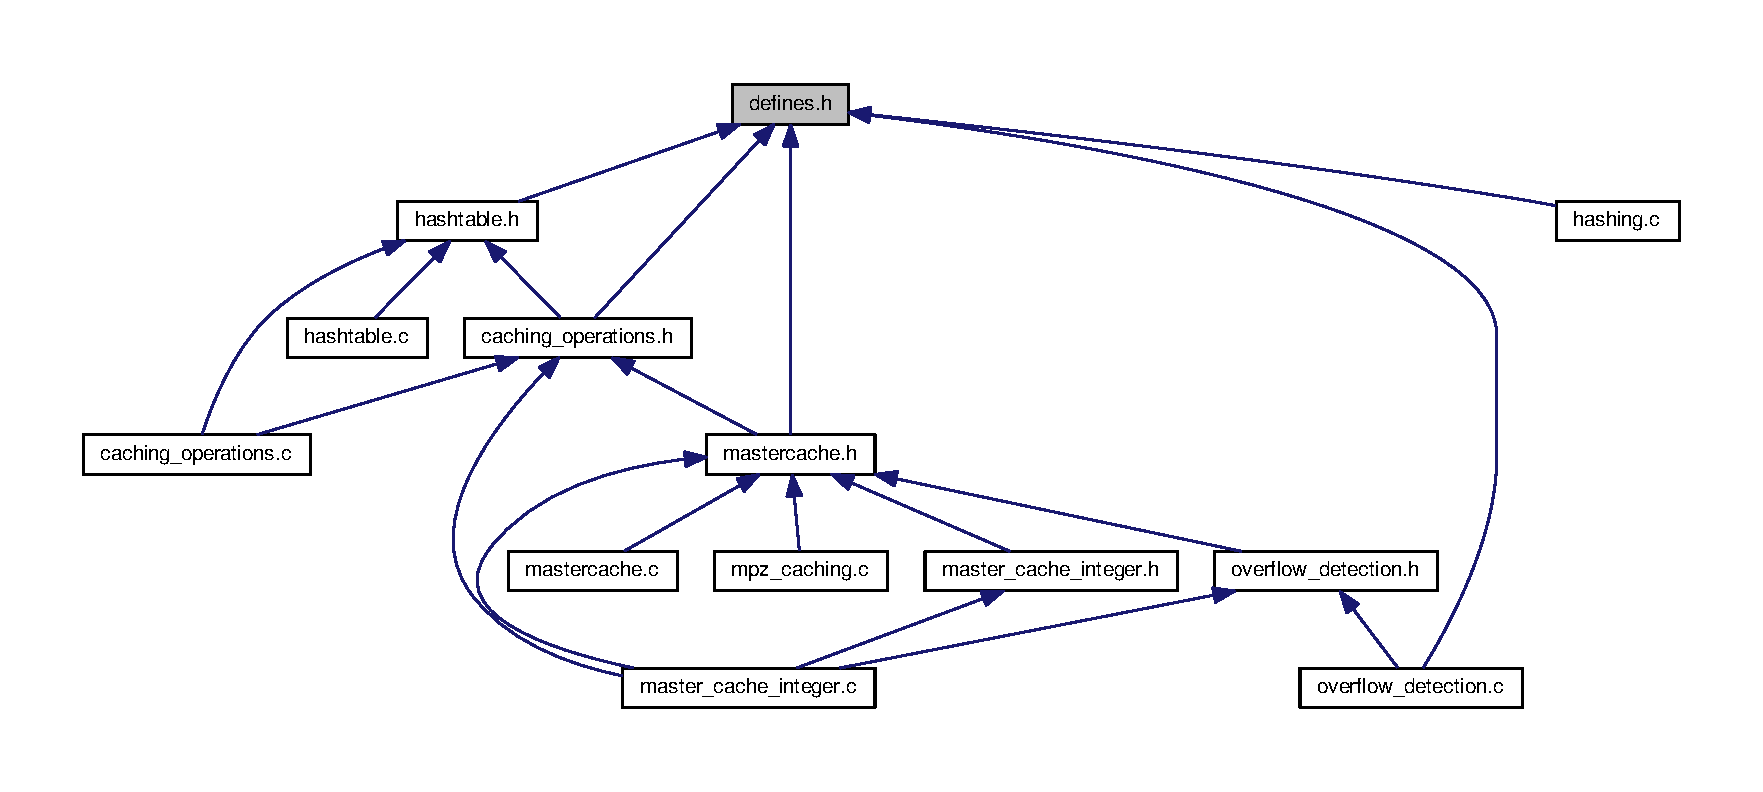
\includegraphics[width=350pt]{defines_8h__dep__incl}
\end{center}
\end{figure}
\subsection*{Macros}
\begin{DoxyCompactItemize}
\item 
\#define \hyperlink{defines_8h_a4ad9728365e70dea0b97d88a14c62710}{cached\+Int\+\_\+\+M\+AX}~(int64\+\_\+t)2$^\wedge$62-\/2
\item 
\#define \hyperlink{defines_8h_ad0a5ef5f0a3a61ddbc2d75a02d8e36e5}{cached\+Int\+\_\+\+M\+IN}~(int64\+\_\+t)-\/(2$^\wedge$62-\/2)
\item 
\#define \hyperlink{defines_8h_a18f2a1494a0d643f51839313f03ab1ea}{cached\+Int\+\_\+\+S\+I\+GN}~63
\item 
\#define \hyperlink{defines_8h_a4d3c17db9bb1b4c9a1a6bdf71d16195a}{cached\+Int\+\_\+\+Is\+ID}~62
\item 
\#define \hyperlink{defines_8h_a1dd941e838c33dd491826fa498bc37b0}{hashtable\+\_\+\+R\+A\+T\+IO}~0.\+4
\item 
\#define \hyperlink{defines_8h_a1d7a097d98759ea37675266376c63e99}{N\+U\+M\+B\+E\+R\+\_\+\+HF}~3
\item 
\#define \hyperlink{defines_8h_ac179eef68bcc694aa0ef8dd1eb09950b}{S\+H\+I\+FT}~((uint64\+\_\+t)1 $<$$<$ \hyperlink{defines_8h_a4d3c17db9bb1b4c9a1a6bdf71d16195a}{cached\+Int\+\_\+\+Is\+ID})
\item 
\#define \hyperlink{defines_8h_aa27c29fc6f203aac29fb3632a0bafda5}{N\+EG}~((uint64\+\_\+t)1 $<$$<$ \hyperlink{defines_8h_a18f2a1494a0d643f51839313f03ab1ea}{cached\+Int\+\_\+\+S\+I\+GN})
\end{DoxyCompactItemize}


\subsection{Detailed Description}
general defines for the caching process 

\begin{DoxyAuthor}{Author}
Sandra Hicks 
\end{DoxyAuthor}


\subsection{Macro Definition Documentation}
\index{defines.\+h@{defines.\+h}!cached\+Int\+\_\+\+Is\+ID@{cached\+Int\+\_\+\+Is\+ID}}
\index{cached\+Int\+\_\+\+Is\+ID@{cached\+Int\+\_\+\+Is\+ID}!defines.\+h@{defines.\+h}}
\subsubsection[{\texorpdfstring{cached\+Int\+\_\+\+Is\+ID}{cachedInt_IsID}}]{\setlength{\rightskip}{0pt plus 5cm}\#define cached\+Int\+\_\+\+Is\+ID~62}\hypertarget{defines_8h_a4d3c17db9bb1b4c9a1a6bdf71d16195a}{}\label{defines_8h_a4d3c17db9bb1b4c9a1a6bdf71d16195a}
bitmask to get the position of cached\+Int indicating if it is an ID or number \index{defines.\+h@{defines.\+h}!cached\+Int\+\_\+\+M\+AX@{cached\+Int\+\_\+\+M\+AX}}
\index{cached\+Int\+\_\+\+M\+AX@{cached\+Int\+\_\+\+M\+AX}!defines.\+h@{defines.\+h}}
\subsubsection[{\texorpdfstring{cached\+Int\+\_\+\+M\+AX}{cachedInt_MAX}}]{\setlength{\rightskip}{0pt plus 5cm}\#define cached\+Int\+\_\+\+M\+AX~(int64\+\_\+t)2$^\wedge$62-\/2}\hypertarget{defines_8h_a4ad9728365e70dea0b97d88a14c62710}{}\label{defines_8h_a4ad9728365e70dea0b97d88a14c62710}
maximum size of a cached\+Int \index{defines.\+h@{defines.\+h}!cached\+Int\+\_\+\+M\+IN@{cached\+Int\+\_\+\+M\+IN}}
\index{cached\+Int\+\_\+\+M\+IN@{cached\+Int\+\_\+\+M\+IN}!defines.\+h@{defines.\+h}}
\subsubsection[{\texorpdfstring{cached\+Int\+\_\+\+M\+IN}{cachedInt_MIN}}]{\setlength{\rightskip}{0pt plus 5cm}\#define cached\+Int\+\_\+\+M\+IN~(int64\+\_\+t)-\/(2$^\wedge$62-\/2)}\hypertarget{defines_8h_ad0a5ef5f0a3a61ddbc2d75a02d8e36e5}{}\label{defines_8h_ad0a5ef5f0a3a61ddbc2d75a02d8e36e5}
minimum size of a cached\+Int \index{defines.\+h@{defines.\+h}!cached\+Int\+\_\+\+S\+I\+GN@{cached\+Int\+\_\+\+S\+I\+GN}}
\index{cached\+Int\+\_\+\+S\+I\+GN@{cached\+Int\+\_\+\+S\+I\+GN}!defines.\+h@{defines.\+h}}
\subsubsection[{\texorpdfstring{cached\+Int\+\_\+\+S\+I\+GN}{cachedInt_SIGN}}]{\setlength{\rightskip}{0pt plus 5cm}\#define cached\+Int\+\_\+\+S\+I\+GN~63}\hypertarget{defines_8h_a18f2a1494a0d643f51839313f03ab1ea}{}\label{defines_8h_a18f2a1494a0d643f51839313f03ab1ea}
bitmask to get sign position of cached\+Int \index{defines.\+h@{defines.\+h}!hashtable\+\_\+\+R\+A\+T\+IO@{hashtable\+\_\+\+R\+A\+T\+IO}}
\index{hashtable\+\_\+\+R\+A\+T\+IO@{hashtable\+\_\+\+R\+A\+T\+IO}!defines.\+h@{defines.\+h}}
\subsubsection[{\texorpdfstring{hashtable\+\_\+\+R\+A\+T\+IO}{hashtable_RATIO}}]{\setlength{\rightskip}{0pt plus 5cm}\#define hashtable\+\_\+\+R\+A\+T\+IO~0.\+4}\hypertarget{defines_8h_a1dd941e838c33dd491826fa498bc37b0}{}\label{defines_8h_a1dd941e838c33dd491826fa498bc37b0}
ratio of the size of the hashtable compared to size of cache \index{defines.\+h@{defines.\+h}!N\+EG@{N\+EG}}
\index{N\+EG@{N\+EG}!defines.\+h@{defines.\+h}}
\subsubsection[{\texorpdfstring{N\+EG}{NEG}}]{\setlength{\rightskip}{0pt plus 5cm}\#define N\+EG~((uint64\+\_\+t)1 $<$$<$ {\bf cached\+Int\+\_\+\+S\+I\+GN})}\hypertarget{defines_8h_aa27c29fc6f203aac29fb3632a0bafda5}{}\label{defines_8h_aa27c29fc6f203aac29fb3632a0bafda5}
macro to detect the bit in a cached\+Int which defines if it is positive or negative \index{defines.\+h@{defines.\+h}!N\+U\+M\+B\+E\+R\+\_\+\+HF@{N\+U\+M\+B\+E\+R\+\_\+\+HF}}
\index{N\+U\+M\+B\+E\+R\+\_\+\+HF@{N\+U\+M\+B\+E\+R\+\_\+\+HF}!defines.\+h@{defines.\+h}}
\subsubsection[{\texorpdfstring{N\+U\+M\+B\+E\+R\+\_\+\+HF}{NUMBER_HF}}]{\setlength{\rightskip}{0pt plus 5cm}\#define N\+U\+M\+B\+E\+R\+\_\+\+HF~3}\hypertarget{defines_8h_a1d7a097d98759ea37675266376c63e99}{}\label{defines_8h_a1d7a097d98759ea37675266376c63e99}
number of hash functions \index{defines.\+h@{defines.\+h}!S\+H\+I\+FT@{S\+H\+I\+FT}}
\index{S\+H\+I\+FT@{S\+H\+I\+FT}!defines.\+h@{defines.\+h}}
\subsubsection[{\texorpdfstring{S\+H\+I\+FT}{SHIFT}}]{\setlength{\rightskip}{0pt plus 5cm}\#define S\+H\+I\+FT~((uint64\+\_\+t)1 $<$$<$ {\bf cached\+Int\+\_\+\+Is\+ID})}\hypertarget{defines_8h_ac179eef68bcc694aa0ef8dd1eb09950b}{}\label{defines_8h_ac179eef68bcc694aa0ef8dd1eb09950b}
macro to detect the bit in a cached\+Int which defines if it is an id or a number 
\hypertarget{hashing_8c}{}\section{hashing.\+c File Reference}
\label{hashing_8c}\index{hashing.\+c@{hashing.\+c}}


implementation of hash functions on mpz\+\_\+t\textquotesingle{}s  


{\ttfamily \#include $<$sys/types.\+h$>$}\\*
{\ttfamily \#include \char`\"{}defines.\+h\char`\"{}}\\*
{\ttfamily \#include $<$gmp.\+h$>$}\\*
{\ttfamily \#include $<$stdint.\+h$>$}\\*
{\ttfamily \#include $<$inttypes.\+h$>$}\\*
{\ttfamily \#include $<$stdio.\+h$>$}\\*
{\ttfamily \#include \char`\"{}debug.\+h\char`\"{}}\\*
Include dependency graph for hashing.\+c\+:\nopagebreak
\begin{figure}[H]
\begin{center}
\leavevmode
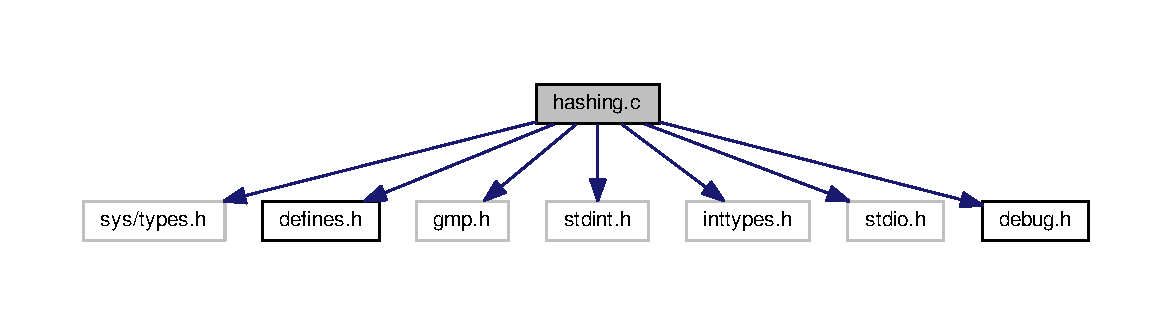
\includegraphics[width=350pt]{hashing_8c__incl}
\end{center}
\end{figure}
\subsection*{Macros}
\begin{DoxyCompactItemize}
\item 
\#define \hyperlink{hashing_8c_a843a032e93d6d54b28933d827eb4c966}{F\+N\+V\+\_\+64\+\_\+\+P\+R\+I\+ME}~((\hyperlink{hashing_8c_ab6714df8881207174e4c0e0b12c32583}{Fnv64\+\_\+t})0x100000001b3\+U\+L\+L)
\item 
\#define \hyperlink{hashing_8c_a97c6e8016ffe540a627163d406059552}{F\+N\+V1\+\_\+64\+\_\+\+I\+N\+IT}~((\hyperlink{hashing_8c_ab6714df8881207174e4c0e0b12c32583}{Fnv64\+\_\+t})0xcbf29ce484222325\+U\+L\+L)
\item 
\#define \hyperlink{hashing_8c_a1eb99785c4898f16341824639f52d50f}{F\+N\+V1\+A\+\_\+64\+\_\+\+I\+N\+IT}~\hyperlink{hashing_8c_a97c6e8016ffe540a627163d406059552}{F\+N\+V1\+\_\+64\+\_\+\+I\+N\+IT}
\end{DoxyCompactItemize}
\subsection*{Typedefs}
\begin{DoxyCompactItemize}
\item 
typedef unsigned \+\_\+\+\_\+int128 \hyperlink{hashing_8c_a396787e5ec029b1205bd3e4cd9763e7d}{uint128\+\_\+t}
\item 
typedef uint64\+\_\+t \hyperlink{hashing_8c_ab6714df8881207174e4c0e0b12c32583}{Fnv64\+\_\+t}
\end{DoxyCompactItemize}
\subsection*{Functions}
\begin{DoxyCompactItemize}
\item 
uint64\+\_\+t \hyperlink{hashing_8c_a2b4c88ee112b98a4964da93fb0c8ab05}{get\+\_\+\+F\+N\+V1a\+\_\+hash} (mpz\+\_\+t myval)
\begin{DoxyCompactList}\small\item\em F\+N\+V1a hashing of an mpz\+\_\+t to a 64 bit unsigned value. \end{DoxyCompactList}\item 
uint64\+\_\+t \hyperlink{hashing_8c_a319e6314e49fb9e23fc8b1667031409a}{get\+\_\+\+Jenkins\+\_\+hash} (mpz\+\_\+t myval)
\begin{DoxyCompactList}\small\item\em (T\+O\+DO) Jenkins Spookyhash hash of a mpz\+\_\+t to a 64 bit unsigned value \end{DoxyCompactList}\item 
uint64\+\_\+t \hyperlink{hashing_8c_a3418cd49ff87c091e401df5c1745f8c0}{get\+\_\+lookup3\+\_\+hash} (mpz\+\_\+t myval)
\begin{DoxyCompactList}\small\item\em (T\+O\+DO) Jenkins lookup3 hash of a mpz\+\_\+t to a 64 bit unsigned value \end{DoxyCompactList}\item 
uint64\+\_\+t \hyperlink{hashing_8c_a8c95fa7a682da0f000d85afbaaf28d83}{get\+\_\+\+Sip\+\_\+hash} (mpz\+\_\+t myval)
\begin{DoxyCompactList}\small\item\em (T\+O\+DO) Siphash hash of a mpz\+\_\+t to a 64 bit unsigned value \end{DoxyCompactList}\item 
uint64\+\_\+t \hyperlink{hashing_8c_ae1fc6aab0474de396ac9abe0ef6e6466}{get\+\_\+\+Murmur\+\_\+hash} (mpz\+\_\+t myval)
\begin{DoxyCompactList}\small\item\em Murmur hash of a mpz\+\_\+t to a 64 bit unsigned value. \end{DoxyCompactList}\item 
uint64\+\_\+t \hyperlink{hashing_8c_a8a8dd73303711a6884acad72b0caa968}{get\+\_\+\+C\+R\+C\+\_\+hash} (mpz\+\_\+t myval)
\begin{DoxyCompactList}\small\item\em C\+RC hash of a mpz\+\_\+t to a 64 bit unsigned value. \end{DoxyCompactList}\item 
uint64\+\_\+t \hyperlink{hashing_8c_af44c8e6918384ae4ab580b7b5976eca9}{Cantor\+\_\+pairing\+\_\+function\+\_\+int64} (uint64\+\_\+t v1, uint64\+\_\+t v2)
\begin{DoxyCompactList}\small\item\em apply Cantor pairing function to uint64\+\_\+t \end{DoxyCompactList}\item 
void \hyperlink{hashing_8c_a6fa8f477d6b93a5a0c4753a75bd3cc8b}{Cantor\+\_\+pairing\+\_\+function\+\_\+mpz} (mpz\+\_\+t v1, mpz\+\_\+t v2, mpz\+\_\+t res)
\begin{DoxyCompactList}\small\item\em apply Cantor pairing function to mpz\+\_\+t \end{DoxyCompactList}\end{DoxyCompactItemize}


\subsection{Detailed Description}
implementation of hash functions on mpz\+\_\+t\textquotesingle{}s 

\begin{DoxyAuthor}{Author}
Sandra Hicks 
\end{DoxyAuthor}


\subsection{Macro Definition Documentation}
\index{hashing.\+c@{hashing.\+c}!F\+N\+V1\+\_\+64\+\_\+\+I\+N\+IT@{F\+N\+V1\+\_\+64\+\_\+\+I\+N\+IT}}
\index{F\+N\+V1\+\_\+64\+\_\+\+I\+N\+IT@{F\+N\+V1\+\_\+64\+\_\+\+I\+N\+IT}!hashing.\+c@{hashing.\+c}}
\subsubsection[{\texorpdfstring{F\+N\+V1\+\_\+64\+\_\+\+I\+N\+IT}{FNV1_64_INIT}}]{\setlength{\rightskip}{0pt plus 5cm}\#define F\+N\+V1\+\_\+64\+\_\+\+I\+N\+IT~(({\bf Fnv64\+\_\+t})0xcbf29ce484222325\+U\+L\+L)}\hypertarget{hashing_8c_a97c6e8016ffe540a627163d406059552}{}\label{hashing_8c_a97c6e8016ffe540a627163d406059552}
init value for F\+N\+V1 \index{hashing.\+c@{hashing.\+c}!F\+N\+V1\+A\+\_\+64\+\_\+\+I\+N\+IT@{F\+N\+V1\+A\+\_\+64\+\_\+\+I\+N\+IT}}
\index{F\+N\+V1\+A\+\_\+64\+\_\+\+I\+N\+IT@{F\+N\+V1\+A\+\_\+64\+\_\+\+I\+N\+IT}!hashing.\+c@{hashing.\+c}}
\subsubsection[{\texorpdfstring{F\+N\+V1\+A\+\_\+64\+\_\+\+I\+N\+IT}{FNV1A_64_INIT}}]{\setlength{\rightskip}{0pt plus 5cm}\#define F\+N\+V1\+A\+\_\+64\+\_\+\+I\+N\+IT~{\bf F\+N\+V1\+\_\+64\+\_\+\+I\+N\+IT}}\hypertarget{hashing_8c_a1eb99785c4898f16341824639f52d50f}{}\label{hashing_8c_a1eb99785c4898f16341824639f52d50f}
init value for F\+N\+V1a \index{hashing.\+c@{hashing.\+c}!F\+N\+V\+\_\+64\+\_\+\+P\+R\+I\+ME@{F\+N\+V\+\_\+64\+\_\+\+P\+R\+I\+ME}}
\index{F\+N\+V\+\_\+64\+\_\+\+P\+R\+I\+ME@{F\+N\+V\+\_\+64\+\_\+\+P\+R\+I\+ME}!hashing.\+c@{hashing.\+c}}
\subsubsection[{\texorpdfstring{F\+N\+V\+\_\+64\+\_\+\+P\+R\+I\+ME}{FNV_64_PRIME}}]{\setlength{\rightskip}{0pt plus 5cm}\#define F\+N\+V\+\_\+64\+\_\+\+P\+R\+I\+ME~(({\bf Fnv64\+\_\+t})0x100000001b3\+U\+L\+L)}\hypertarget{hashing_8c_a843a032e93d6d54b28933d827eb4c966}{}\label{hashing_8c_a843a032e93d6d54b28933d827eb4c966}
special prime for F\+N\+V1a 

\subsection{Typedef Documentation}
\index{hashing.\+c@{hashing.\+c}!Fnv64\+\_\+t@{Fnv64\+\_\+t}}
\index{Fnv64\+\_\+t@{Fnv64\+\_\+t}!hashing.\+c@{hashing.\+c}}
\subsubsection[{\texorpdfstring{Fnv64\+\_\+t}{Fnv64_t}}]{\setlength{\rightskip}{0pt plus 5cm}typedef uint64\+\_\+t {\bf Fnv64\+\_\+t}}\hypertarget{hashing_8c_ab6714df8881207174e4c0e0b12c32583}{}\label{hashing_8c_ab6714df8881207174e4c0e0b12c32583}
use uint64\+\_\+t for implementing the F\+N\+V1a algorithm \index{hashing.\+c@{hashing.\+c}!uint128\+\_\+t@{uint128\+\_\+t}}
\index{uint128\+\_\+t@{uint128\+\_\+t}!hashing.\+c@{hashing.\+c}}
\subsubsection[{\texorpdfstring{uint128\+\_\+t}{uint128_t}}]{\setlength{\rightskip}{0pt plus 5cm}typedef unsigned \+\_\+\+\_\+int128 {\bf uint128\+\_\+t}}\hypertarget{hashing_8c_a396787e5ec029b1205bd3e4cd9763e7d}{}\label{hashing_8c_a396787e5ec029b1205bd3e4cd9763e7d}
need a uint128\+\_\+t value 

\subsection{Function Documentation}
\index{hashing.\+c@{hashing.\+c}!Cantor\+\_\+pairing\+\_\+function\+\_\+int64@{Cantor\+\_\+pairing\+\_\+function\+\_\+int64}}
\index{Cantor\+\_\+pairing\+\_\+function\+\_\+int64@{Cantor\+\_\+pairing\+\_\+function\+\_\+int64}!hashing.\+c@{hashing.\+c}}
\subsubsection[{\texorpdfstring{Cantor\+\_\+pairing\+\_\+function\+\_\+int64(uint64\+\_\+t v1, uint64\+\_\+t v2)}{Cantor_pairing_function_int64(uint64_t v1, uint64_t v2)}}]{\setlength{\rightskip}{0pt plus 5cm}uint64\+\_\+t Cantor\+\_\+pairing\+\_\+function\+\_\+int64 (
\begin{DoxyParamCaption}
\item[{uint64\+\_\+t}]{v1, }
\item[{uint64\+\_\+t}]{v2}
\end{DoxyParamCaption}
)}\hypertarget{hashing_8c_af44c8e6918384ae4ab580b7b5976eca9}{}\label{hashing_8c_af44c8e6918384ae4ab580b7b5976eca9}


apply Cantor pairing function to uint64\+\_\+t 


\begin{DoxyParams}{Parameters}
{\em v1} & operand 1 \\
\hline
{\em v2} & operand 2 \\
\hline
\end{DoxyParams}
\begin{DoxyReturn}{Returns}
result 
\end{DoxyReturn}
\index{hashing.\+c@{hashing.\+c}!Cantor\+\_\+pairing\+\_\+function\+\_\+mpz@{Cantor\+\_\+pairing\+\_\+function\+\_\+mpz}}
\index{Cantor\+\_\+pairing\+\_\+function\+\_\+mpz@{Cantor\+\_\+pairing\+\_\+function\+\_\+mpz}!hashing.\+c@{hashing.\+c}}
\subsubsection[{\texorpdfstring{Cantor\+\_\+pairing\+\_\+function\+\_\+mpz(mpz\+\_\+t v1, mpz\+\_\+t v2, mpz\+\_\+t res)}{Cantor_pairing_function_mpz(mpz_t v1, mpz_t v2, mpz_t res)}}]{\setlength{\rightskip}{0pt plus 5cm}void Cantor\+\_\+pairing\+\_\+function\+\_\+mpz (
\begin{DoxyParamCaption}
\item[{mpz\+\_\+t}]{v1, }
\item[{mpz\+\_\+t}]{v2, }
\item[{mpz\+\_\+t}]{res}
\end{DoxyParamCaption}
)}\hypertarget{hashing_8c_a6fa8f477d6b93a5a0c4753a75bd3cc8b}{}\label{hashing_8c_a6fa8f477d6b93a5a0c4753a75bd3cc8b}


apply Cantor pairing function to mpz\+\_\+t 


\begin{DoxyParams}{Parameters}
{\em v1} & operand 1 \\
\hline
{\em v2} & operand 2 \\
\hline
{\em res} & resulting mpz\+\_\+t \\
\hline
\end{DoxyParams}
\index{hashing.\+c@{hashing.\+c}!get\+\_\+\+C\+R\+C\+\_\+hash@{get\+\_\+\+C\+R\+C\+\_\+hash}}
\index{get\+\_\+\+C\+R\+C\+\_\+hash@{get\+\_\+\+C\+R\+C\+\_\+hash}!hashing.\+c@{hashing.\+c}}
\subsubsection[{\texorpdfstring{get\+\_\+\+C\+R\+C\+\_\+hash(mpz\+\_\+t myval)}{get_CRC_hash(mpz_t myval)}}]{\setlength{\rightskip}{0pt plus 5cm}uint64\+\_\+t get\+\_\+\+C\+R\+C\+\_\+hash (
\begin{DoxyParamCaption}
\item[{mpz\+\_\+t}]{myval}
\end{DoxyParamCaption}
)}\hypertarget{hashing_8c_a8a8dd73303711a6884acad72b0caa968}{}\label{hashing_8c_a8a8dd73303711a6884acad72b0caa968}


C\+RC hash of a mpz\+\_\+t to a 64 bit unsigned value. 


\begin{DoxyParams}{Parameters}
{\em myval} & mpz\+\_\+t to be hashed \\
\hline
\end{DoxyParams}
\begin{DoxyReturn}{Returns}
hash value 
\end{DoxyReturn}
\index{hashing.\+c@{hashing.\+c}!get\+\_\+\+F\+N\+V1a\+\_\+hash@{get\+\_\+\+F\+N\+V1a\+\_\+hash}}
\index{get\+\_\+\+F\+N\+V1a\+\_\+hash@{get\+\_\+\+F\+N\+V1a\+\_\+hash}!hashing.\+c@{hashing.\+c}}
\subsubsection[{\texorpdfstring{get\+\_\+\+F\+N\+V1a\+\_\+hash(mpz\+\_\+t myval)}{get_FNV1a_hash(mpz_t myval)}}]{\setlength{\rightskip}{0pt plus 5cm}uint64\+\_\+t get\+\_\+\+F\+N\+V1a\+\_\+hash (
\begin{DoxyParamCaption}
\item[{mpz\+\_\+t}]{myval}
\end{DoxyParamCaption}
)}\hypertarget{hashing_8c_a2b4c88ee112b98a4964da93fb0c8ab05}{}\label{hashing_8c_a2b4c88ee112b98a4964da93fb0c8ab05}


F\+N\+V1a hashing of an mpz\+\_\+t to a 64 bit unsigned value. 


\begin{DoxyParams}{Parameters}
{\em myval} & mpz\+\_\+t to be hashed \\
\hline
\end{DoxyParams}
\begin{DoxyReturn}{Returns}
hash value 
\end{DoxyReturn}
\index{hashing.\+c@{hashing.\+c}!get\+\_\+\+Jenkins\+\_\+hash@{get\+\_\+\+Jenkins\+\_\+hash}}
\index{get\+\_\+\+Jenkins\+\_\+hash@{get\+\_\+\+Jenkins\+\_\+hash}!hashing.\+c@{hashing.\+c}}
\subsubsection[{\texorpdfstring{get\+\_\+\+Jenkins\+\_\+hash(mpz\+\_\+t myval)}{get_Jenkins_hash(mpz_t myval)}}]{\setlength{\rightskip}{0pt plus 5cm}uint64\+\_\+t get\+\_\+\+Jenkins\+\_\+hash (
\begin{DoxyParamCaption}
\item[{mpz\+\_\+t}]{myval}
\end{DoxyParamCaption}
)}\hypertarget{hashing_8c_a319e6314e49fb9e23fc8b1667031409a}{}\label{hashing_8c_a319e6314e49fb9e23fc8b1667031409a}


(T\+O\+DO) Jenkins Spookyhash hash of a mpz\+\_\+t to a 64 bit unsigned value 


\begin{DoxyParams}{Parameters}
{\em myval} & mpz\+\_\+t to be hashed \\
\hline
\end{DoxyParams}
\begin{DoxyReturn}{Returns}
hash value 
\end{DoxyReturn}
\index{hashing.\+c@{hashing.\+c}!get\+\_\+lookup3\+\_\+hash@{get\+\_\+lookup3\+\_\+hash}}
\index{get\+\_\+lookup3\+\_\+hash@{get\+\_\+lookup3\+\_\+hash}!hashing.\+c@{hashing.\+c}}
\subsubsection[{\texorpdfstring{get\+\_\+lookup3\+\_\+hash(mpz\+\_\+t myval)}{get_lookup3_hash(mpz_t myval)}}]{\setlength{\rightskip}{0pt plus 5cm}uint64\+\_\+t get\+\_\+lookup3\+\_\+hash (
\begin{DoxyParamCaption}
\item[{mpz\+\_\+t}]{myval}
\end{DoxyParamCaption}
)}\hypertarget{hashing_8c_a3418cd49ff87c091e401df5c1745f8c0}{}\label{hashing_8c_a3418cd49ff87c091e401df5c1745f8c0}


(T\+O\+DO) Jenkins lookup3 hash of a mpz\+\_\+t to a 64 bit unsigned value 


\begin{DoxyParams}{Parameters}
{\em myval} & mpz\+\_\+t to be hashed \\
\hline
\end{DoxyParams}
\begin{DoxyReturn}{Returns}
hash value 
\end{DoxyReturn}
\index{hashing.\+c@{hashing.\+c}!get\+\_\+\+Murmur\+\_\+hash@{get\+\_\+\+Murmur\+\_\+hash}}
\index{get\+\_\+\+Murmur\+\_\+hash@{get\+\_\+\+Murmur\+\_\+hash}!hashing.\+c@{hashing.\+c}}
\subsubsection[{\texorpdfstring{get\+\_\+\+Murmur\+\_\+hash(mpz\+\_\+t myval)}{get_Murmur_hash(mpz_t myval)}}]{\setlength{\rightskip}{0pt plus 5cm}uint64\+\_\+t get\+\_\+\+Murmur\+\_\+hash (
\begin{DoxyParamCaption}
\item[{mpz\+\_\+t}]{myval}
\end{DoxyParamCaption}
)}\hypertarget{hashing_8c_ae1fc6aab0474de396ac9abe0ef6e6466}{}\label{hashing_8c_ae1fc6aab0474de396ac9abe0ef6e6466}


Murmur hash of a mpz\+\_\+t to a 64 bit unsigned value. 


\begin{DoxyParams}{Parameters}
{\em myval} & mpz\+\_\+t to be hashed \\
\hline
\end{DoxyParams}
\begin{DoxyReturn}{Returns}
hash value 
\end{DoxyReturn}
\index{hashing.\+c@{hashing.\+c}!get\+\_\+\+Sip\+\_\+hash@{get\+\_\+\+Sip\+\_\+hash}}
\index{get\+\_\+\+Sip\+\_\+hash@{get\+\_\+\+Sip\+\_\+hash}!hashing.\+c@{hashing.\+c}}
\subsubsection[{\texorpdfstring{get\+\_\+\+Sip\+\_\+hash(mpz\+\_\+t myval)}{get_Sip_hash(mpz_t myval)}}]{\setlength{\rightskip}{0pt plus 5cm}uint64\+\_\+t get\+\_\+\+Sip\+\_\+hash (
\begin{DoxyParamCaption}
\item[{mpz\+\_\+t}]{myval}
\end{DoxyParamCaption}
)}\hypertarget{hashing_8c_a8c95fa7a682da0f000d85afbaaf28d83}{}\label{hashing_8c_a8c95fa7a682da0f000d85afbaaf28d83}


(T\+O\+DO) Siphash hash of a mpz\+\_\+t to a 64 bit unsigned value 


\begin{DoxyParams}{Parameters}
{\em myval} & mpz\+\_\+t to be hashed \\
\hline
\end{DoxyParams}
\begin{DoxyReturn}{Returns}
hash value 
\end{DoxyReturn}

\hypertarget{hashing_8h}{}\section{hashing.\+h File Reference}
\label{hashing_8h}\index{hashing.\+h@{hashing.\+h}}


header for implementation of hash functions on mpz\+\_\+t\textquotesingle{}s  


{\ttfamily \#include $<$stdint.\+h$>$}\\*
{\ttfamily \#include $<$gmp.\+h$>$}\\*
Include dependency graph for hashing.\+h\+:\nopagebreak
\begin{figure}[H]
\begin{center}
\leavevmode
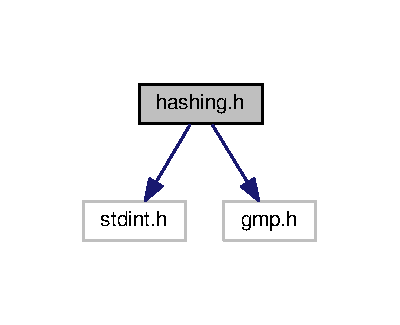
\includegraphics[width=192pt]{hashing_8h__incl}
\end{center}
\end{figure}
This graph shows which files directly or indirectly include this file\+:\nopagebreak
\begin{figure}[H]
\begin{center}
\leavevmode
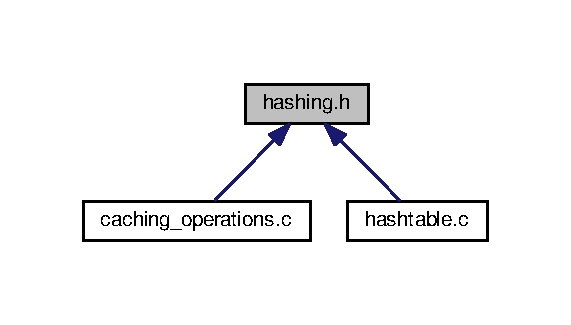
\includegraphics[width=274pt]{hashing_8h__dep__incl}
\end{center}
\end{figure}
\subsection*{Functions}
\begin{DoxyCompactItemize}
\item 
uint64\+\_\+t \hyperlink{hashing_8h_a2b4c88ee112b98a4964da93fb0c8ab05}{get\+\_\+\+F\+N\+V1a\+\_\+hash} (mpz\+\_\+t myval)
\begin{DoxyCompactList}\small\item\em F\+N\+V1a hashing of an mpz\+\_\+t to a 64 bit unsigned value. \end{DoxyCompactList}\item 
uint64\+\_\+t \hyperlink{hashing_8h_a319e6314e49fb9e23fc8b1667031409a}{get\+\_\+\+Jenkins\+\_\+hash} (mpz\+\_\+t myval)
\begin{DoxyCompactList}\small\item\em (T\+O\+DO) Jenkins Spookyhash hash of a mpz\+\_\+t to a 64 bit unsigned value \end{DoxyCompactList}\item 
uint64\+\_\+t \hyperlink{hashing_8h_a3418cd49ff87c091e401df5c1745f8c0}{get\+\_\+lookup3\+\_\+hash} (mpz\+\_\+t myval)
\begin{DoxyCompactList}\small\item\em (T\+O\+DO) Jenkins lookup3 hash of a mpz\+\_\+t to a 64 bit unsigned value \end{DoxyCompactList}\item 
uint64\+\_\+t \hyperlink{hashing_8h_a8c95fa7a682da0f000d85afbaaf28d83}{get\+\_\+\+Sip\+\_\+hash} (mpz\+\_\+t myval)
\begin{DoxyCompactList}\small\item\em (T\+O\+DO) Siphash hash of a mpz\+\_\+t to a 64 bit unsigned value \end{DoxyCompactList}\item 
uint64\+\_\+t \hyperlink{hashing_8h_ae1fc6aab0474de396ac9abe0ef6e6466}{get\+\_\+\+Murmur\+\_\+hash} (mpz\+\_\+t myval)
\begin{DoxyCompactList}\small\item\em Murmur hash of a mpz\+\_\+t to a 64 bit unsigned value. \end{DoxyCompactList}\item 
uint64\+\_\+t \hyperlink{hashing_8h_a8a8dd73303711a6884acad72b0caa968}{get\+\_\+\+C\+R\+C\+\_\+hash} (mpz\+\_\+t myval)
\begin{DoxyCompactList}\small\item\em C\+RC hash of a mpz\+\_\+t to a 64 bit unsigned value. \end{DoxyCompactList}\item 
void \hyperlink{hashing_8h_a6fa8f477d6b93a5a0c4753a75bd3cc8b}{Cantor\+\_\+pairing\+\_\+function\+\_\+mpz} (mpz\+\_\+t v1, mpz\+\_\+t v2, mpz\+\_\+t res)
\begin{DoxyCompactList}\small\item\em apply Cantor pairing function to mpz\+\_\+t \end{DoxyCompactList}\item 
uint64\+\_\+t \hyperlink{hashing_8h_af44c8e6918384ae4ab580b7b5976eca9}{Cantor\+\_\+pairing\+\_\+function\+\_\+int64} (uint64\+\_\+t v1, uint64\+\_\+t v2)
\begin{DoxyCompactList}\small\item\em apply Cantor pairing function to uint64\+\_\+t \end{DoxyCompactList}\end{DoxyCompactItemize}


\subsection{Detailed Description}
header for implementation of hash functions on mpz\+\_\+t\textquotesingle{}s 

\begin{DoxyAuthor}{Author}
Sandra Hicks 
\end{DoxyAuthor}


\subsection{Function Documentation}
\index{hashing.\+h@{hashing.\+h}!Cantor\+\_\+pairing\+\_\+function\+\_\+int64@{Cantor\+\_\+pairing\+\_\+function\+\_\+int64}}
\index{Cantor\+\_\+pairing\+\_\+function\+\_\+int64@{Cantor\+\_\+pairing\+\_\+function\+\_\+int64}!hashing.\+h@{hashing.\+h}}
\subsubsection[{\texorpdfstring{Cantor\+\_\+pairing\+\_\+function\+\_\+int64(uint64\+\_\+t v1, uint64\+\_\+t v2)}{Cantor_pairing_function_int64(uint64_t v1, uint64_t v2)}}]{\setlength{\rightskip}{0pt plus 5cm}uint64\+\_\+t Cantor\+\_\+pairing\+\_\+function\+\_\+int64 (
\begin{DoxyParamCaption}
\item[{uint64\+\_\+t}]{v1, }
\item[{uint64\+\_\+t}]{v2}
\end{DoxyParamCaption}
)}\hypertarget{hashing_8h_af44c8e6918384ae4ab580b7b5976eca9}{}\label{hashing_8h_af44c8e6918384ae4ab580b7b5976eca9}


apply Cantor pairing function to uint64\+\_\+t 


\begin{DoxyParams}{Parameters}
{\em v1} & operand 1 \\
\hline
{\em v2} & operand 2 \\
\hline
\end{DoxyParams}
\begin{DoxyReturn}{Returns}
result 
\end{DoxyReturn}
\index{hashing.\+h@{hashing.\+h}!Cantor\+\_\+pairing\+\_\+function\+\_\+mpz@{Cantor\+\_\+pairing\+\_\+function\+\_\+mpz}}
\index{Cantor\+\_\+pairing\+\_\+function\+\_\+mpz@{Cantor\+\_\+pairing\+\_\+function\+\_\+mpz}!hashing.\+h@{hashing.\+h}}
\subsubsection[{\texorpdfstring{Cantor\+\_\+pairing\+\_\+function\+\_\+mpz(mpz\+\_\+t v1, mpz\+\_\+t v2, mpz\+\_\+t res)}{Cantor_pairing_function_mpz(mpz_t v1, mpz_t v2, mpz_t res)}}]{\setlength{\rightskip}{0pt plus 5cm}void Cantor\+\_\+pairing\+\_\+function\+\_\+mpz (
\begin{DoxyParamCaption}
\item[{mpz\+\_\+t}]{v1, }
\item[{mpz\+\_\+t}]{v2, }
\item[{mpz\+\_\+t}]{res}
\end{DoxyParamCaption}
)}\hypertarget{hashing_8h_a6fa8f477d6b93a5a0c4753a75bd3cc8b}{}\label{hashing_8h_a6fa8f477d6b93a5a0c4753a75bd3cc8b}


apply Cantor pairing function to mpz\+\_\+t 


\begin{DoxyParams}{Parameters}
{\em v1} & operand 1 \\
\hline
{\em v2} & operand 2 \\
\hline
{\em res} & resulting mpz\+\_\+t \\
\hline
\end{DoxyParams}
\index{hashing.\+h@{hashing.\+h}!get\+\_\+\+C\+R\+C\+\_\+hash@{get\+\_\+\+C\+R\+C\+\_\+hash}}
\index{get\+\_\+\+C\+R\+C\+\_\+hash@{get\+\_\+\+C\+R\+C\+\_\+hash}!hashing.\+h@{hashing.\+h}}
\subsubsection[{\texorpdfstring{get\+\_\+\+C\+R\+C\+\_\+hash(mpz\+\_\+t myval)}{get_CRC_hash(mpz_t myval)}}]{\setlength{\rightskip}{0pt plus 5cm}uint64\+\_\+t get\+\_\+\+C\+R\+C\+\_\+hash (
\begin{DoxyParamCaption}
\item[{mpz\+\_\+t}]{myval}
\end{DoxyParamCaption}
)}\hypertarget{hashing_8h_a8a8dd73303711a6884acad72b0caa968}{}\label{hashing_8h_a8a8dd73303711a6884acad72b0caa968}


C\+RC hash of a mpz\+\_\+t to a 64 bit unsigned value. 


\begin{DoxyParams}{Parameters}
{\em myval} & mpz\+\_\+t to be hashed \\
\hline
\end{DoxyParams}
\begin{DoxyReturn}{Returns}
hash value 
\end{DoxyReturn}
\index{hashing.\+h@{hashing.\+h}!get\+\_\+\+F\+N\+V1a\+\_\+hash@{get\+\_\+\+F\+N\+V1a\+\_\+hash}}
\index{get\+\_\+\+F\+N\+V1a\+\_\+hash@{get\+\_\+\+F\+N\+V1a\+\_\+hash}!hashing.\+h@{hashing.\+h}}
\subsubsection[{\texorpdfstring{get\+\_\+\+F\+N\+V1a\+\_\+hash(mpz\+\_\+t myval)}{get_FNV1a_hash(mpz_t myval)}}]{\setlength{\rightskip}{0pt plus 5cm}uint64\+\_\+t get\+\_\+\+F\+N\+V1a\+\_\+hash (
\begin{DoxyParamCaption}
\item[{mpz\+\_\+t}]{myval}
\end{DoxyParamCaption}
)}\hypertarget{hashing_8h_a2b4c88ee112b98a4964da93fb0c8ab05}{}\label{hashing_8h_a2b4c88ee112b98a4964da93fb0c8ab05}


F\+N\+V1a hashing of an mpz\+\_\+t to a 64 bit unsigned value. 


\begin{DoxyParams}{Parameters}
{\em myval} & mpz\+\_\+t to be hashed \\
\hline
\end{DoxyParams}
\begin{DoxyReturn}{Returns}
hash value 
\end{DoxyReturn}
\index{hashing.\+h@{hashing.\+h}!get\+\_\+\+Jenkins\+\_\+hash@{get\+\_\+\+Jenkins\+\_\+hash}}
\index{get\+\_\+\+Jenkins\+\_\+hash@{get\+\_\+\+Jenkins\+\_\+hash}!hashing.\+h@{hashing.\+h}}
\subsubsection[{\texorpdfstring{get\+\_\+\+Jenkins\+\_\+hash(mpz\+\_\+t myval)}{get_Jenkins_hash(mpz_t myval)}}]{\setlength{\rightskip}{0pt plus 5cm}uint64\+\_\+t get\+\_\+\+Jenkins\+\_\+hash (
\begin{DoxyParamCaption}
\item[{mpz\+\_\+t}]{myval}
\end{DoxyParamCaption}
)}\hypertarget{hashing_8h_a319e6314e49fb9e23fc8b1667031409a}{}\label{hashing_8h_a319e6314e49fb9e23fc8b1667031409a}


(T\+O\+DO) Jenkins Spookyhash hash of a mpz\+\_\+t to a 64 bit unsigned value 


\begin{DoxyParams}{Parameters}
{\em myval} & mpz\+\_\+t to be hashed \\
\hline
\end{DoxyParams}
\begin{DoxyReturn}{Returns}
hash value 
\end{DoxyReturn}
\index{hashing.\+h@{hashing.\+h}!get\+\_\+lookup3\+\_\+hash@{get\+\_\+lookup3\+\_\+hash}}
\index{get\+\_\+lookup3\+\_\+hash@{get\+\_\+lookup3\+\_\+hash}!hashing.\+h@{hashing.\+h}}
\subsubsection[{\texorpdfstring{get\+\_\+lookup3\+\_\+hash(mpz\+\_\+t myval)}{get_lookup3_hash(mpz_t myval)}}]{\setlength{\rightskip}{0pt plus 5cm}uint64\+\_\+t get\+\_\+lookup3\+\_\+hash (
\begin{DoxyParamCaption}
\item[{mpz\+\_\+t}]{myval}
\end{DoxyParamCaption}
)}\hypertarget{hashing_8h_a3418cd49ff87c091e401df5c1745f8c0}{}\label{hashing_8h_a3418cd49ff87c091e401df5c1745f8c0}


(T\+O\+DO) Jenkins lookup3 hash of a mpz\+\_\+t to a 64 bit unsigned value 


\begin{DoxyParams}{Parameters}
{\em myval} & mpz\+\_\+t to be hashed \\
\hline
\end{DoxyParams}
\begin{DoxyReturn}{Returns}
hash value 
\end{DoxyReturn}
\index{hashing.\+h@{hashing.\+h}!get\+\_\+\+Murmur\+\_\+hash@{get\+\_\+\+Murmur\+\_\+hash}}
\index{get\+\_\+\+Murmur\+\_\+hash@{get\+\_\+\+Murmur\+\_\+hash}!hashing.\+h@{hashing.\+h}}
\subsubsection[{\texorpdfstring{get\+\_\+\+Murmur\+\_\+hash(mpz\+\_\+t myval)}{get_Murmur_hash(mpz_t myval)}}]{\setlength{\rightskip}{0pt plus 5cm}uint64\+\_\+t get\+\_\+\+Murmur\+\_\+hash (
\begin{DoxyParamCaption}
\item[{mpz\+\_\+t}]{myval}
\end{DoxyParamCaption}
)}\hypertarget{hashing_8h_ae1fc6aab0474de396ac9abe0ef6e6466}{}\label{hashing_8h_ae1fc6aab0474de396ac9abe0ef6e6466}


Murmur hash of a mpz\+\_\+t to a 64 bit unsigned value. 


\begin{DoxyParams}{Parameters}
{\em myval} & mpz\+\_\+t to be hashed \\
\hline
\end{DoxyParams}
\begin{DoxyReturn}{Returns}
hash value 
\end{DoxyReturn}
\index{hashing.\+h@{hashing.\+h}!get\+\_\+\+Sip\+\_\+hash@{get\+\_\+\+Sip\+\_\+hash}}
\index{get\+\_\+\+Sip\+\_\+hash@{get\+\_\+\+Sip\+\_\+hash}!hashing.\+h@{hashing.\+h}}
\subsubsection[{\texorpdfstring{get\+\_\+\+Sip\+\_\+hash(mpz\+\_\+t myval)}{get_Sip_hash(mpz_t myval)}}]{\setlength{\rightskip}{0pt plus 5cm}uint64\+\_\+t get\+\_\+\+Sip\+\_\+hash (
\begin{DoxyParamCaption}
\item[{mpz\+\_\+t}]{myval}
\end{DoxyParamCaption}
)}\hypertarget{hashing_8h_a8c95fa7a682da0f000d85afbaaf28d83}{}\label{hashing_8h_a8c95fa7a682da0f000d85afbaaf28d83}


(T\+O\+DO) Siphash hash of a mpz\+\_\+t to a 64 bit unsigned value 


\begin{DoxyParams}{Parameters}
{\em myval} & mpz\+\_\+t to be hashed \\
\hline
\end{DoxyParams}
\begin{DoxyReturn}{Returns}
hash value 
\end{DoxyReturn}

\hypertarget{hashtable_8c}{}\section{hashtable.\+c File Reference}
\label{hashtable_8c}\index{hashtable.\+c@{hashtable.\+c}}


hash table implementation  


{\ttfamily \#include \char`\"{}hashtable.\+h\char`\"{}}\\*
{\ttfamily \#include \char`\"{}hashing.\+h\char`\"{}}\\*
{\ttfamily \#include \char`\"{}mpz\+\_\+caching.\+h\char`\"{}}\\*
{\ttfamily \#include $<$stdint.\+h$>$}\\*
{\ttfamily \#include $<$stdlib.\+h$>$}\\*
{\ttfamily \#include $<$stdio.\+h$>$}\\*
{\ttfamily \#include $<$inttypes.\+h$>$}\\*
Include dependency graph for hashtable.\+c\+:\nopagebreak
\begin{figure}[H]
\begin{center}
\leavevmode
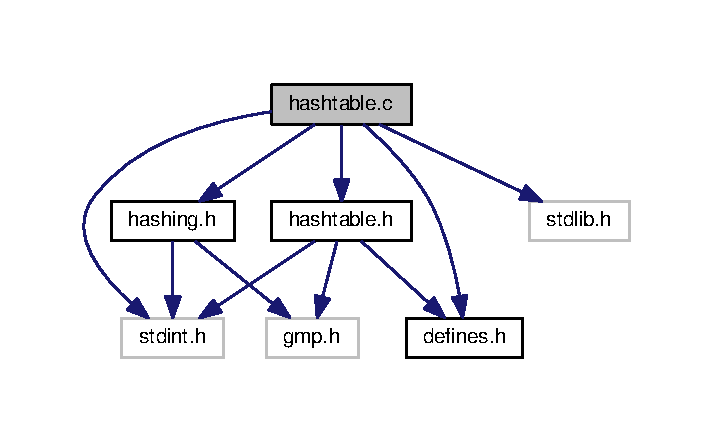
\includegraphics[width=350pt]{hashtable_8c__incl}
\end{center}
\end{figure}
\subsection*{Functions}
\begin{DoxyCompactItemize}
\item 
void \hyperlink{hashtable_8c_a8f4aa8473391505b303072098b101285}{init\+\_\+hashtable} (\hyperlink{structHashtable}{Hashtable} $\ast$ht, uint64\+\_\+t size)
\begin{DoxyCompactList}\small\item\em initialization of the hash table \end{DoxyCompactList}\item 
void \hyperlink{hashtable_8c_a31e50f67c07fb1a475268694bfd5743d}{delete\+\_\+hashtable} (\hyperlink{structHashtable}{Hashtable} $\ast$ht)
\begin{DoxyCompactList}\small\item\em deletion of the hash table and all its underlying data structures \end{DoxyCompactList}\item 
void \hyperlink{hashtable_8c_a3999323c0facade24699b869058ddeb7}{insert\+\_\+element} (\hyperlink{structHashtable}{Hashtable} $\ast$ht, uint64\+\_\+t id, uint64\+\_\+t $\ast$hashes)
\begin{DoxyCompactList}\small\item\em insertion method for an element in the hash table \end{DoxyCompactList}\item 
uint64\+\_\+t \hyperlink{hashtable_8c_aa2cdb80b044d66f091e6cad114e633b9}{exists\+\_\+element} (\hyperlink{structHashtable}{Hashtable} $\ast$ht, uint64\+\_\+t $\ast$hashes, mpz\+\_\+t element, \hyperlink{structmpz__t__cache}{mpz\+\_\+t\+\_\+cache} $\ast$cache)
\begin{DoxyCompactList}\small\item\em check existence of an element \end{DoxyCompactList}\item 
void \hyperlink{hashtable_8c_a7198d8653365a8e7b187bbcb49bab4aa}{get\+\_\+k\+\_\+hashes} (mpz\+\_\+t val, uint64\+\_\+t $\ast$hashes)
\begin{DoxyCompactList}\small\item\em function to calculate the multiple hash values for an mpz\+\_\+t element \end{DoxyCompactList}\item 
void \hyperlink{hashtable_8c_af267b5c3e0669ad9844482299eb9dce0}{get\+\_\+k\+\_\+hashes\+\_\+cpf} (mpz\+\_\+t val1, mpz\+\_\+t val2, uint64\+\_\+t $\ast$hashes)
\begin{DoxyCompactList}\small\item\em function to calculate multiple hashes for a tupel of mpz\+\_\+t\textquotesingle{}s after applying Cantor Pairing function \end{DoxyCompactList}\item 
void \hyperlink{hashtable_8c_a1758c25104d2433ec0fb68861baaa330}{init\+\_\+hashtable\+\_\+binary} (\hyperlink{structHashtable__binary}{Hashtable\+\_\+binary} $\ast$ht, uint64\+\_\+t size)
\begin{DoxyCompactList}\small\item\em initialization of a hashtable for (mpz\+\_\+t x mpz\+\_\+t) -\/$>$ mpz\+\_\+t \end{DoxyCompactList}\item 
void \hyperlink{hashtable_8c_a99e3e52694edc6e5396bc93bcdb2d0eb}{delete\+\_\+hashtable\+\_\+binary} (\hyperlink{structHashtable__binary}{Hashtable\+\_\+binary} $\ast$ht)
\begin{DoxyCompactList}\small\item\em deletion of hash table and all underlying data structures \end{DoxyCompactList}\item 
void \hyperlink{hashtable_8c_a8d6049bccb0ee7c582dd8190c9e0530d}{insert\+\_\+element\+\_\+binary} (\hyperlink{structHashtable__binary}{Hashtable\+\_\+binary} $\ast$ht, uint64\+\_\+t id\+\_\+op1, uint64\+\_\+t id\+\_\+op2, uint64\+\_\+t id\+\_\+res, uint64\+\_\+t $\ast$extra\+\_\+info, uint64\+\_\+t $\ast$hashes)
\begin{DoxyCompactList}\small\item\em insert a mapping (mpz\+\_\+t x mpz\+\_\+t) -\/$>$ mpz\+\_\+t in hashtable \end{DoxyCompactList}\item 
uint64\+\_\+t \hyperlink{hashtable_8c_a640832720182207089e4e7156ffcac6d}{exists\+\_\+element\+\_\+binary} (\hyperlink{structHashtable__binary}{Hashtable\+\_\+binary} $\ast$ht, uint64\+\_\+t $\ast$hashes, mpz\+\_\+t op1, mpz\+\_\+t op2, \hyperlink{structmpz__t__cache}{mpz\+\_\+t\+\_\+cache} $\ast$cache, uint64\+\_\+t $\ast$extra\+\_\+info)
\begin{DoxyCompactList}\small\item\em function to check if a mapping (mpz\+\_\+t x mpz\+\_\+t) -\/$>$ mpz\+\_\+t exists in the hash table \end{DoxyCompactList}\end{DoxyCompactItemize}


\subsection{Detailed Description}
hash table implementation 

\begin{DoxyAuthor}{Author}
Sandra Hicks 
\end{DoxyAuthor}


\subsection{Function Documentation}
\index{hashtable.\+c@{hashtable.\+c}!delete\+\_\+hashtable@{delete\+\_\+hashtable}}
\index{delete\+\_\+hashtable@{delete\+\_\+hashtable}!hashtable.\+c@{hashtable.\+c}}
\subsubsection[{\texorpdfstring{delete\+\_\+hashtable(\+Hashtable $\ast$ht)}{delete_hashtable(Hashtable *ht)}}]{\setlength{\rightskip}{0pt plus 5cm}void delete\+\_\+hashtable (
\begin{DoxyParamCaption}
\item[{{\bf Hashtable} $\ast$}]{ht}
\end{DoxyParamCaption}
)}\hypertarget{hashtable_8c_a31e50f67c07fb1a475268694bfd5743d}{}\label{hashtable_8c_a31e50f67c07fb1a475268694bfd5743d}


deletion of the hash table and all its underlying data structures 


\begin{DoxyParams}{Parameters}
{\em ht} & pointer to hash table \\
\hline
\end{DoxyParams}
\index{hashtable.\+c@{hashtable.\+c}!delete\+\_\+hashtable\+\_\+binary@{delete\+\_\+hashtable\+\_\+binary}}
\index{delete\+\_\+hashtable\+\_\+binary@{delete\+\_\+hashtable\+\_\+binary}!hashtable.\+c@{hashtable.\+c}}
\subsubsection[{\texorpdfstring{delete\+\_\+hashtable\+\_\+binary(\+Hashtable\+\_\+binary $\ast$ht)}{delete_hashtable_binary(Hashtable_binary *ht)}}]{\setlength{\rightskip}{0pt plus 5cm}void delete\+\_\+hashtable\+\_\+binary (
\begin{DoxyParamCaption}
\item[{{\bf Hashtable\+\_\+binary} $\ast$}]{ht}
\end{DoxyParamCaption}
)}\hypertarget{hashtable_8c_a99e3e52694edc6e5396bc93bcdb2d0eb}{}\label{hashtable_8c_a99e3e52694edc6e5396bc93bcdb2d0eb}


deletion of hash table and all underlying data structures 


\begin{DoxyParams}{Parameters}
{\em ht} & pointer to hash table \\
\hline
\end{DoxyParams}
\index{hashtable.\+c@{hashtable.\+c}!exists\+\_\+element@{exists\+\_\+element}}
\index{exists\+\_\+element@{exists\+\_\+element}!hashtable.\+c@{hashtable.\+c}}
\subsubsection[{\texorpdfstring{exists\+\_\+element(\+Hashtable $\ast$ht, uint64\+\_\+t $\ast$hashes, mpz\+\_\+t element, mpz\+\_\+t\+\_\+cache $\ast$cache)}{exists_element(Hashtable *ht, uint64_t *hashes, mpz_t element, mpz_t_cache *cache)}}]{\setlength{\rightskip}{0pt plus 5cm}uint64\+\_\+t exists\+\_\+element (
\begin{DoxyParamCaption}
\item[{{\bf Hashtable} $\ast$}]{ht, }
\item[{uint64\+\_\+t $\ast$}]{hashes, }
\item[{mpz\+\_\+t}]{element, }
\item[{{\bf mpz\+\_\+t\+\_\+cache} $\ast$}]{cache}
\end{DoxyParamCaption}
)}\hypertarget{hashtable_8c_aa2cdb80b044d66f091e6cad114e633b9}{}\label{hashtable_8c_aa2cdb80b044d66f091e6cad114e633b9}


check existence of an element 


\begin{DoxyParams}{Parameters}
{\em ht} & pointer to hash table \\
\hline
{\em hashes} & array of hash values for the element \\
\hline
{\em element} & mpz\+\_\+t to search for \\
\hline
{\em cache} & pointer to singleton cache \\
\hline
\end{DoxyParams}
\begin{DoxyReturn}{Returns}
id if existent, if not return 0 
\end{DoxyReturn}
\index{hashtable.\+c@{hashtable.\+c}!exists\+\_\+element\+\_\+binary@{exists\+\_\+element\+\_\+binary}}
\index{exists\+\_\+element\+\_\+binary@{exists\+\_\+element\+\_\+binary}!hashtable.\+c@{hashtable.\+c}}
\subsubsection[{\texorpdfstring{exists\+\_\+element\+\_\+binary(\+Hashtable\+\_\+binary $\ast$ht, uint64\+\_\+t $\ast$hashes, mpz\+\_\+t op1, mpz\+\_\+t op2, mpz\+\_\+t\+\_\+cache $\ast$cache, uint64\+\_\+t $\ast$extra\+\_\+info)}{exists_element_binary(Hashtable_binary *ht, uint64_t *hashes, mpz_t op1, mpz_t op2, mpz_t_cache *cache, uint64_t *extra_info)}}]{\setlength{\rightskip}{0pt plus 5cm}uint64\+\_\+t exists\+\_\+element\+\_\+binary (
\begin{DoxyParamCaption}
\item[{{\bf Hashtable\+\_\+binary} $\ast$}]{ht, }
\item[{uint64\+\_\+t $\ast$}]{hashes, }
\item[{mpz\+\_\+t}]{op1, }
\item[{mpz\+\_\+t}]{op2, }
\item[{{\bf mpz\+\_\+t\+\_\+cache} $\ast$}]{cache, }
\item[{uint64\+\_\+t $\ast$}]{extra\+\_\+info}
\end{DoxyParamCaption}
)}\hypertarget{hashtable_8c_a640832720182207089e4e7156ffcac6d}{}\label{hashtable_8c_a640832720182207089e4e7156ffcac6d}


function to check if a mapping (mpz\+\_\+t x mpz\+\_\+t) -\/$>$ mpz\+\_\+t exists in the hash table 


\begin{DoxyParams}{Parameters}
{\em ht} & pointer to hash table \\
\hline
{\em hashes} & array of hashes \\
\hline
{\em op1} & first operator \\
\hline
{\em op2} & second operator \\
\hline
{\em cache} & pointer to singleton mpz\+\_\+t cache \\
\hline
{\em extra\+\_\+info} & id of extra info of found element, stays null if none exists \\
\hline
\end{DoxyParams}
\begin{DoxyReturn}{Returns}
id if found, 0 if not existent 
\end{DoxyReturn}
\index{hashtable.\+c@{hashtable.\+c}!get\+\_\+k\+\_\+hashes@{get\+\_\+k\+\_\+hashes}}
\index{get\+\_\+k\+\_\+hashes@{get\+\_\+k\+\_\+hashes}!hashtable.\+c@{hashtable.\+c}}
\subsubsection[{\texorpdfstring{get\+\_\+k\+\_\+hashes(mpz\+\_\+t val, uint64\+\_\+t $\ast$hashes)}{get_k_hashes(mpz_t val, uint64_t *hashes)}}]{\setlength{\rightskip}{0pt plus 5cm}void get\+\_\+k\+\_\+hashes (
\begin{DoxyParamCaption}
\item[{mpz\+\_\+t}]{val, }
\item[{uint64\+\_\+t $\ast$}]{hashes}
\end{DoxyParamCaption}
)}\hypertarget{hashtable_8c_a7198d8653365a8e7b187bbcb49bab4aa}{}\label{hashtable_8c_a7198d8653365a8e7b187bbcb49bab4aa}


function to calculate the multiple hash values for an mpz\+\_\+t element 


\begin{DoxyParams}{Parameters}
{\em val} & mpz\+\_\+t value to hash \\
\hline
{\em hashes} & pointer to array of hashes to fill \\
\hline
\end{DoxyParams}
\index{hashtable.\+c@{hashtable.\+c}!get\+\_\+k\+\_\+hashes\+\_\+cpf@{get\+\_\+k\+\_\+hashes\+\_\+cpf}}
\index{get\+\_\+k\+\_\+hashes\+\_\+cpf@{get\+\_\+k\+\_\+hashes\+\_\+cpf}!hashtable.\+c@{hashtable.\+c}}
\subsubsection[{\texorpdfstring{get\+\_\+k\+\_\+hashes\+\_\+cpf(mpz\+\_\+t val1, mpz\+\_\+t val2, uint64\+\_\+t $\ast$hashes)}{get_k_hashes_cpf(mpz_t val1, mpz_t val2, uint64_t *hashes)}}]{\setlength{\rightskip}{0pt plus 5cm}void get\+\_\+k\+\_\+hashes\+\_\+cpf (
\begin{DoxyParamCaption}
\item[{mpz\+\_\+t}]{val1, }
\item[{mpz\+\_\+t}]{val2, }
\item[{uint64\+\_\+t $\ast$}]{hashes}
\end{DoxyParamCaption}
)}\hypertarget{hashtable_8c_af267b5c3e0669ad9844482299eb9dce0}{}\label{hashtable_8c_af267b5c3e0669ad9844482299eb9dce0}


function to calculate multiple hashes for a tupel of mpz\+\_\+t\textquotesingle{}s after applying Cantor Pairing function 


\begin{DoxyParams}{Parameters}
{\em val1} & first mpz\+\_\+t \\
\hline
{\em val2} & second mpz\+\_\+t \\
\hline
{\em hashes} & array of hashes to fill \\
\hline
\end{DoxyParams}
\index{hashtable.\+c@{hashtable.\+c}!init\+\_\+hashtable@{init\+\_\+hashtable}}
\index{init\+\_\+hashtable@{init\+\_\+hashtable}!hashtable.\+c@{hashtable.\+c}}
\subsubsection[{\texorpdfstring{init\+\_\+hashtable(\+Hashtable $\ast$ht, uint64\+\_\+t size)}{init_hashtable(Hashtable *ht, uint64_t size)}}]{\setlength{\rightskip}{0pt plus 5cm}void init\+\_\+hashtable (
\begin{DoxyParamCaption}
\item[{{\bf Hashtable} $\ast$}]{ht, }
\item[{uint64\+\_\+t}]{size}
\end{DoxyParamCaption}
)}\hypertarget{hashtable_8c_a8f4aa8473391505b303072098b101285}{}\label{hashtable_8c_a8f4aa8473391505b303072098b101285}


initialization of the hash table 


\begin{DoxyParams}{Parameters}
{\em ht} & pointer to hash table \\
\hline
{\em size} & of the hash table \\
\hline
\end{DoxyParams}
\index{hashtable.\+c@{hashtable.\+c}!init\+\_\+hashtable\+\_\+binary@{init\+\_\+hashtable\+\_\+binary}}
\index{init\+\_\+hashtable\+\_\+binary@{init\+\_\+hashtable\+\_\+binary}!hashtable.\+c@{hashtable.\+c}}
\subsubsection[{\texorpdfstring{init\+\_\+hashtable\+\_\+binary(\+Hashtable\+\_\+binary $\ast$ht, uint64\+\_\+t size)}{init_hashtable_binary(Hashtable_binary *ht, uint64_t size)}}]{\setlength{\rightskip}{0pt plus 5cm}void init\+\_\+hashtable\+\_\+binary (
\begin{DoxyParamCaption}
\item[{{\bf Hashtable\+\_\+binary} $\ast$}]{ht, }
\item[{uint64\+\_\+t}]{size}
\end{DoxyParamCaption}
)}\hypertarget{hashtable_8c_a1758c25104d2433ec0fb68861baaa330}{}\label{hashtable_8c_a1758c25104d2433ec0fb68861baaa330}


initialization of a hashtable for (mpz\+\_\+t x mpz\+\_\+t) -\/$>$ mpz\+\_\+t 


\begin{DoxyParams}{Parameters}
{\em ht} & pointer to hash table \\
\hline
{\em size} & size of hash table \\
\hline
\end{DoxyParams}
\index{hashtable.\+c@{hashtable.\+c}!insert\+\_\+element@{insert\+\_\+element}}
\index{insert\+\_\+element@{insert\+\_\+element}!hashtable.\+c@{hashtable.\+c}}
\subsubsection[{\texorpdfstring{insert\+\_\+element(\+Hashtable $\ast$ht, uint64\+\_\+t id, uint64\+\_\+t $\ast$hashes)}{insert_element(Hashtable *ht, uint64_t id, uint64_t *hashes)}}]{\setlength{\rightskip}{0pt plus 5cm}void insert\+\_\+element (
\begin{DoxyParamCaption}
\item[{{\bf Hashtable} $\ast$}]{ht, }
\item[{uint64\+\_\+t}]{id, }
\item[{uint64\+\_\+t $\ast$}]{hashes}
\end{DoxyParamCaption}
)}\hypertarget{hashtable_8c_a3999323c0facade24699b869058ddeb7}{}\label{hashtable_8c_a3999323c0facade24699b869058ddeb7}


insertion method for an element in the hash table 


\begin{DoxyParams}{Parameters}
{\em ht} & pointer to hash table \\
\hline
{\em id} & id of the mpz\+\_\+t in the singleton cache \\
\hline
{\em hashes} & array of hash values of the mpz\+\_\+t \\
\hline
\end{DoxyParams}
\index{hashtable.\+c@{hashtable.\+c}!insert\+\_\+element\+\_\+binary@{insert\+\_\+element\+\_\+binary}}
\index{insert\+\_\+element\+\_\+binary@{insert\+\_\+element\+\_\+binary}!hashtable.\+c@{hashtable.\+c}}
\subsubsection[{\texorpdfstring{insert\+\_\+element\+\_\+binary(\+Hashtable\+\_\+binary $\ast$ht, uint64\+\_\+t id\+\_\+op1, uint64\+\_\+t id\+\_\+op2, uint64\+\_\+t id\+\_\+res, uint64\+\_\+t $\ast$extra\+\_\+info, uint64\+\_\+t $\ast$hashes)}{insert_element_binary(Hashtable_binary *ht, uint64_t id_op1, uint64_t id_op2, uint64_t id_res, uint64_t *extra_info, uint64_t *hashes)}}]{\setlength{\rightskip}{0pt plus 5cm}void insert\+\_\+element\+\_\+binary (
\begin{DoxyParamCaption}
\item[{{\bf Hashtable\+\_\+binary} $\ast$}]{ht, }
\item[{uint64\+\_\+t}]{id\+\_\+op1, }
\item[{uint64\+\_\+t}]{id\+\_\+op2, }
\item[{uint64\+\_\+t}]{id\+\_\+res, }
\item[{uint64\+\_\+t $\ast$}]{extra\+\_\+info, }
\item[{uint64\+\_\+t $\ast$}]{hashes}
\end{DoxyParamCaption}
)}\hypertarget{hashtable_8c_a8d6049bccb0ee7c582dd8190c9e0530d}{}\label{hashtable_8c_a8d6049bccb0ee7c582dd8190c9e0530d}


insert a mapping (mpz\+\_\+t x mpz\+\_\+t) -\/$>$ mpz\+\_\+t in hashtable 


\begin{DoxyParams}{Parameters}
{\em ht} & pointer to hash table \\
\hline
{\em id\+\_\+op1} & id to first operand in singleton cache \\
\hline
{\em id\+\_\+op2} & id to second operand in singleton cache \\
\hline
{\em id\+\_\+res} & id to result in singleton cache \\
\hline
{\em extra\+\_\+info} & id to extra info in singleton cache (e.\+g. division rest) \\
\hline
{\em hashes} & array of hashes \\
\hline
\end{DoxyParams}

\hypertarget{hashtable_8h}{}\section{hashtable.\+h File Reference}
\label{hashtable_8h}\index{hashtable.\+h@{hashtable.\+h}}


Header for hash table implementation.  


{\ttfamily \#include $<$stdint.\+h$>$}\\*
{\ttfamily \#include \char`\"{}defines.\+h\char`\"{}}\\*
{\ttfamily \#include \char`\"{}mpz\+\_\+caching.\+h\char`\"{}}\\*
{\ttfamily \#include $<$gmp.\+h$>$}\\*
Include dependency graph for hashtable.\+h\+:\nopagebreak
\begin{figure}[H]
\begin{center}
\leavevmode
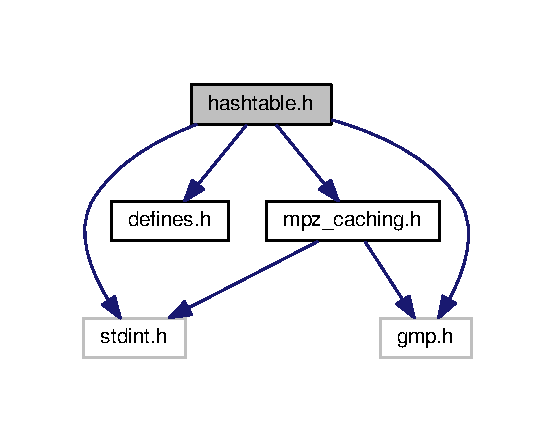
\includegraphics[width=267pt]{hashtable_8h__incl}
\end{center}
\end{figure}
This graph shows which files directly or indirectly include this file\+:\nopagebreak
\begin{figure}[H]
\begin{center}
\leavevmode
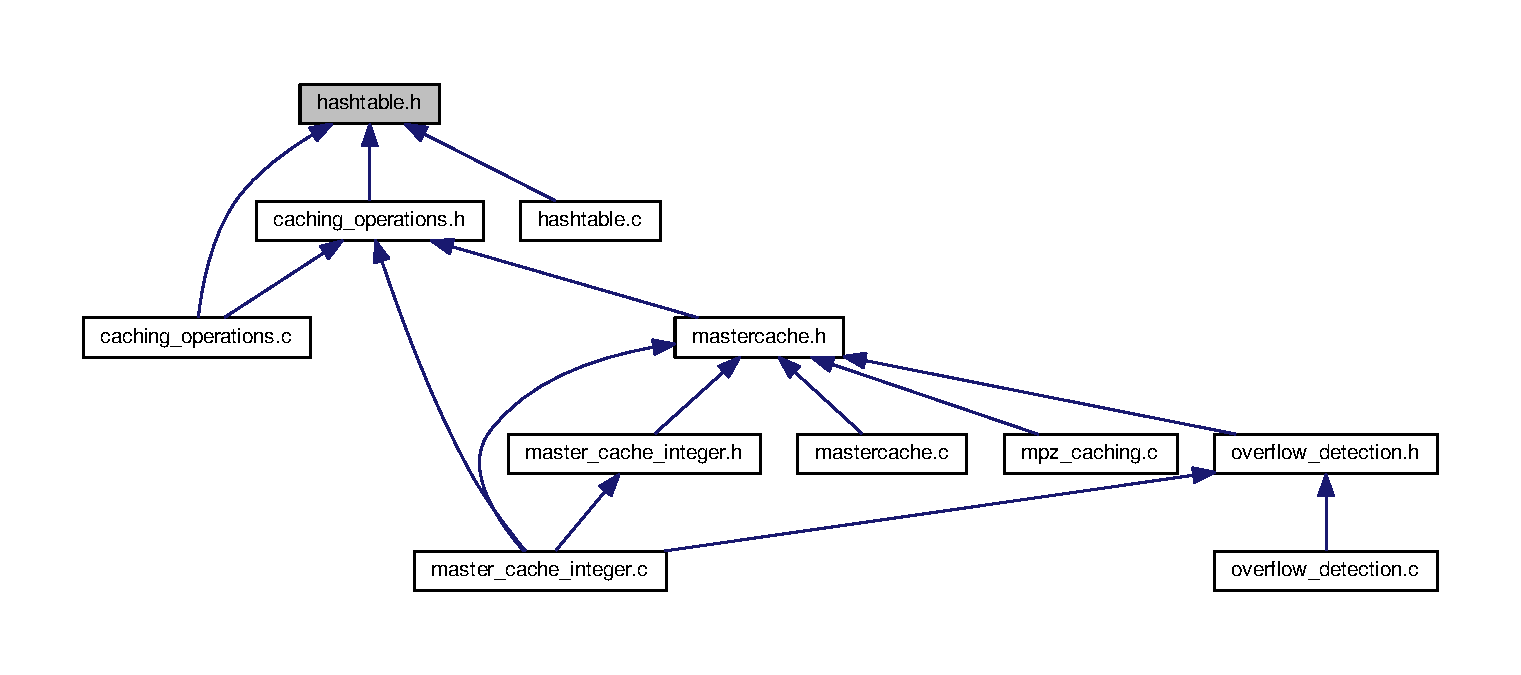
\includegraphics[width=350pt]{hashtable_8h__dep__incl}
\end{center}
\end{figure}
\subsection*{Classes}
\begin{DoxyCompactItemize}
\item 
struct \hyperlink{structcachedIntElement}{cached\+Int\+Element}
\begin{DoxyCompactList}\small\item\em Element of the hash table. \end{DoxyCompactList}\item 
struct \hyperlink{structcachedIntList}{cached\+Int\+List}
\begin{DoxyCompactList}\small\item\em List of Elements in one slot of the hash table. \end{DoxyCompactList}\item 
struct \hyperlink{structHashtable}{Hashtable}
\begin{DoxyCompactList}\small\item\em hash table \end{DoxyCompactList}\item 
struct \hyperlink{structcachedIntElement__binary}{cached\+Int\+Element\+\_\+binary}
\begin{DoxyCompactList}\small\item\em element of hash table binary mapping \end{DoxyCompactList}\item 
struct \hyperlink{structcachedIntList__binary}{cached\+Int\+List\+\_\+binary}
\begin{DoxyCompactList}\small\item\em list of elements in one slot of the hash table binary mapping \end{DoxyCompactList}\item 
struct \hyperlink{structHashtable__binary}{Hashtable\+\_\+binary}
\begin{DoxyCompactList}\small\item\em hash table binary mapping \end{DoxyCompactList}\end{DoxyCompactItemize}
\subsection*{Typedefs}
\begin{DoxyCompactItemize}
\item 
typedef struct \hyperlink{structcachedIntElement}{cached\+Int\+Element} \hyperlink{hashtable_8h_a44bf679bfa4c7678ebfd153172bb5268}{cached\+Int\+Element}\hypertarget{hashtable_8h_a44bf679bfa4c7678ebfd153172bb5268}{}\label{hashtable_8h_a44bf679bfa4c7678ebfd153172bb5268}

\begin{DoxyCompactList}\small\item\em Element of the hash table. \end{DoxyCompactList}\item 
typedef struct \hyperlink{structcachedIntList}{cached\+Int\+List} \hyperlink{hashtable_8h_a50866be81e04ce297cac4ded795314b2}{cached\+Int\+List}\hypertarget{hashtable_8h_a50866be81e04ce297cac4ded795314b2}{}\label{hashtable_8h_a50866be81e04ce297cac4ded795314b2}

\begin{DoxyCompactList}\small\item\em List of Elements in one slot of the hash table. \end{DoxyCompactList}\item 
typedef struct \hyperlink{structHashtable}{Hashtable} \hyperlink{hashtable_8h_a9ef29b69618421bbfaad15efeea75201}{Hashtable}\hypertarget{hashtable_8h_a9ef29b69618421bbfaad15efeea75201}{}\label{hashtable_8h_a9ef29b69618421bbfaad15efeea75201}

\begin{DoxyCompactList}\small\item\em hash table \end{DoxyCompactList}\item 
typedef struct \hyperlink{structcachedIntElement__binary}{cached\+Int\+Element\+\_\+binary} \hyperlink{hashtable_8h_a6c52337ae6ced738d9ad1044c62d821e}{cached\+Int\+Element\+\_\+binary}\hypertarget{hashtable_8h_a6c52337ae6ced738d9ad1044c62d821e}{}\label{hashtable_8h_a6c52337ae6ced738d9ad1044c62d821e}

\begin{DoxyCompactList}\small\item\em element of hash table binary mapping \end{DoxyCompactList}\item 
typedef struct \hyperlink{structcachedIntList__binary}{cached\+Int\+List\+\_\+binary} \hyperlink{hashtable_8h_a051c88e7c88c188a75b017f2dab2031c}{cached\+Int\+List\+\_\+binary}\hypertarget{hashtable_8h_a051c88e7c88c188a75b017f2dab2031c}{}\label{hashtable_8h_a051c88e7c88c188a75b017f2dab2031c}

\begin{DoxyCompactList}\small\item\em list of elements in one slot of the hash table binary mapping \end{DoxyCompactList}\item 
typedef struct \hyperlink{structHashtable__binary}{Hashtable\+\_\+binary} \hyperlink{hashtable_8h_a54f40ceb8fdc52f64990012096a7c7b1}{Hashtable\+\_\+binary}\hypertarget{hashtable_8h_a54f40ceb8fdc52f64990012096a7c7b1}{}\label{hashtable_8h_a54f40ceb8fdc52f64990012096a7c7b1}

\begin{DoxyCompactList}\small\item\em hash table binary mapping \end{DoxyCompactList}\end{DoxyCompactItemize}
\subsection*{Functions}
\begin{DoxyCompactItemize}
\item 
void \hyperlink{hashtable_8h_a8f4aa8473391505b303072098b101285}{init\+\_\+hashtable} (\hyperlink{structHashtable}{Hashtable} $\ast$ht, uint64\+\_\+t size)
\begin{DoxyCompactList}\small\item\em initialization of the hash table \end{DoxyCompactList}\item 
void \hyperlink{hashtable_8h_a31e50f67c07fb1a475268694bfd5743d}{delete\+\_\+hashtable} (\hyperlink{structHashtable}{Hashtable} $\ast$ht)
\begin{DoxyCompactList}\small\item\em deletion of the hash table and all its underlying data structures \end{DoxyCompactList}\item 
void \hyperlink{hashtable_8h_a3999323c0facade24699b869058ddeb7}{insert\+\_\+element} (\hyperlink{structHashtable}{Hashtable} $\ast$ht, uint64\+\_\+t id, uint64\+\_\+t $\ast$hashes)
\begin{DoxyCompactList}\small\item\em insertion method for an element in the hash table \end{DoxyCompactList}\item 
uint64\+\_\+t \hyperlink{hashtable_8h_aa2cdb80b044d66f091e6cad114e633b9}{exists\+\_\+element} (\hyperlink{structHashtable}{Hashtable} $\ast$ht, uint64\+\_\+t $\ast$hashes, mpz\+\_\+t element, \hyperlink{structmpz__t__cache}{mpz\+\_\+t\+\_\+cache} $\ast$cache)
\begin{DoxyCompactList}\small\item\em check existence of an element \end{DoxyCompactList}\item 
void \hyperlink{hashtable_8h_a7198d8653365a8e7b187bbcb49bab4aa}{get\+\_\+k\+\_\+hashes} (mpz\+\_\+t val, uint64\+\_\+t $\ast$hashes)
\begin{DoxyCompactList}\small\item\em function to calculate the multiple hash values for an mpz\+\_\+t element \end{DoxyCompactList}\item 
void \hyperlink{hashtable_8h_a1758c25104d2433ec0fb68861baaa330}{init\+\_\+hashtable\+\_\+binary} (\hyperlink{structHashtable__binary}{Hashtable\+\_\+binary} $\ast$ht, uint64\+\_\+t size)
\begin{DoxyCompactList}\small\item\em initialization of a hashtable for (mpz\+\_\+t x mpz\+\_\+t) -\/$>$ mpz\+\_\+t \end{DoxyCompactList}\item 
void \hyperlink{hashtable_8h_a99e3e52694edc6e5396bc93bcdb2d0eb}{delete\+\_\+hashtable\+\_\+binary} (\hyperlink{structHashtable__binary}{Hashtable\+\_\+binary} $\ast$ht)
\begin{DoxyCompactList}\small\item\em deletion of hash table and all underlying data structures \end{DoxyCompactList}\item 
void \hyperlink{hashtable_8h_a8d6049bccb0ee7c582dd8190c9e0530d}{insert\+\_\+element\+\_\+binary} (\hyperlink{structHashtable__binary}{Hashtable\+\_\+binary} $\ast$ht, uint64\+\_\+t id\+\_\+op1, uint64\+\_\+t id\+\_\+op2, uint64\+\_\+t id\+\_\+res, uint64\+\_\+t $\ast$extra\+\_\+info, uint64\+\_\+t $\ast$hashes)
\begin{DoxyCompactList}\small\item\em insert a mapping (mpz\+\_\+t x mpz\+\_\+t) -\/$>$ mpz\+\_\+t in hashtable \end{DoxyCompactList}\item 
uint64\+\_\+t \hyperlink{hashtable_8h_a640832720182207089e4e7156ffcac6d}{exists\+\_\+element\+\_\+binary} (\hyperlink{structHashtable__binary}{Hashtable\+\_\+binary} $\ast$ht, uint64\+\_\+t $\ast$hashes, mpz\+\_\+t op1, mpz\+\_\+t op2, \hyperlink{structmpz__t__cache}{mpz\+\_\+t\+\_\+cache} $\ast$cache, uint64\+\_\+t $\ast$extra\+\_\+info)
\begin{DoxyCompactList}\small\item\em function to check if a mapping (mpz\+\_\+t x mpz\+\_\+t) -\/$>$ mpz\+\_\+t exists in the hash table \end{DoxyCompactList}\item 
void \hyperlink{hashtable_8h_af267b5c3e0669ad9844482299eb9dce0}{get\+\_\+k\+\_\+hashes\+\_\+cpf} (mpz\+\_\+t val1, mpz\+\_\+t val2, uint64\+\_\+t $\ast$hashes)
\begin{DoxyCompactList}\small\item\em function to calculate multiple hashes for a tupel of mpz\+\_\+t\textquotesingle{}s after applying Cantor Pairing function \end{DoxyCompactList}\end{DoxyCompactItemize}


\subsection{Detailed Description}
Header for hash table implementation. 

\begin{DoxyAuthor}{Author}
Sandra Hicks 
\end{DoxyAuthor}


\subsection{Function Documentation}
\index{hashtable.\+h@{hashtable.\+h}!delete\+\_\+hashtable@{delete\+\_\+hashtable}}
\index{delete\+\_\+hashtable@{delete\+\_\+hashtable}!hashtable.\+h@{hashtable.\+h}}
\subsubsection[{\texorpdfstring{delete\+\_\+hashtable(\+Hashtable $\ast$ht)}{delete_hashtable(Hashtable *ht)}}]{\setlength{\rightskip}{0pt plus 5cm}void delete\+\_\+hashtable (
\begin{DoxyParamCaption}
\item[{{\bf Hashtable} $\ast$}]{ht}
\end{DoxyParamCaption}
)}\hypertarget{hashtable_8h_a31e50f67c07fb1a475268694bfd5743d}{}\label{hashtable_8h_a31e50f67c07fb1a475268694bfd5743d}


deletion of the hash table and all its underlying data structures 


\begin{DoxyParams}{Parameters}
{\em ht} & pointer to hash table \\
\hline
\end{DoxyParams}
\index{hashtable.\+h@{hashtable.\+h}!delete\+\_\+hashtable\+\_\+binary@{delete\+\_\+hashtable\+\_\+binary}}
\index{delete\+\_\+hashtable\+\_\+binary@{delete\+\_\+hashtable\+\_\+binary}!hashtable.\+h@{hashtable.\+h}}
\subsubsection[{\texorpdfstring{delete\+\_\+hashtable\+\_\+binary(\+Hashtable\+\_\+binary $\ast$ht)}{delete_hashtable_binary(Hashtable_binary *ht)}}]{\setlength{\rightskip}{0pt plus 5cm}void delete\+\_\+hashtable\+\_\+binary (
\begin{DoxyParamCaption}
\item[{{\bf Hashtable\+\_\+binary} $\ast$}]{ht}
\end{DoxyParamCaption}
)}\hypertarget{hashtable_8h_a99e3e52694edc6e5396bc93bcdb2d0eb}{}\label{hashtable_8h_a99e3e52694edc6e5396bc93bcdb2d0eb}


deletion of hash table and all underlying data structures 


\begin{DoxyParams}{Parameters}
{\em ht} & pointer to hash table \\
\hline
\end{DoxyParams}
\index{hashtable.\+h@{hashtable.\+h}!exists\+\_\+element@{exists\+\_\+element}}
\index{exists\+\_\+element@{exists\+\_\+element}!hashtable.\+h@{hashtable.\+h}}
\subsubsection[{\texorpdfstring{exists\+\_\+element(\+Hashtable $\ast$ht, uint64\+\_\+t $\ast$hashes, mpz\+\_\+t element, mpz\+\_\+t\+\_\+cache $\ast$cache)}{exists_element(Hashtable *ht, uint64_t *hashes, mpz_t element, mpz_t_cache *cache)}}]{\setlength{\rightskip}{0pt plus 5cm}uint64\+\_\+t exists\+\_\+element (
\begin{DoxyParamCaption}
\item[{{\bf Hashtable} $\ast$}]{ht, }
\item[{uint64\+\_\+t $\ast$}]{hashes, }
\item[{mpz\+\_\+t}]{element, }
\item[{{\bf mpz\+\_\+t\+\_\+cache} $\ast$}]{cache}
\end{DoxyParamCaption}
)}\hypertarget{hashtable_8h_aa2cdb80b044d66f091e6cad114e633b9}{}\label{hashtable_8h_aa2cdb80b044d66f091e6cad114e633b9}


check existence of an element 


\begin{DoxyParams}{Parameters}
{\em ht} & pointer to hash table \\
\hline
{\em hashes} & array of hash values for the element \\
\hline
{\em element} & mpz\+\_\+t to search for \\
\hline
{\em cache} & pointer to singleton cache \\
\hline
\end{DoxyParams}
\begin{DoxyReturn}{Returns}
id if existent, if not return 0 
\end{DoxyReturn}
\index{hashtable.\+h@{hashtable.\+h}!exists\+\_\+element\+\_\+binary@{exists\+\_\+element\+\_\+binary}}
\index{exists\+\_\+element\+\_\+binary@{exists\+\_\+element\+\_\+binary}!hashtable.\+h@{hashtable.\+h}}
\subsubsection[{\texorpdfstring{exists\+\_\+element\+\_\+binary(\+Hashtable\+\_\+binary $\ast$ht, uint64\+\_\+t $\ast$hashes, mpz\+\_\+t op1, mpz\+\_\+t op2, mpz\+\_\+t\+\_\+cache $\ast$cache, uint64\+\_\+t $\ast$extra\+\_\+info)}{exists_element_binary(Hashtable_binary *ht, uint64_t *hashes, mpz_t op1, mpz_t op2, mpz_t_cache *cache, uint64_t *extra_info)}}]{\setlength{\rightskip}{0pt plus 5cm}uint64\+\_\+t exists\+\_\+element\+\_\+binary (
\begin{DoxyParamCaption}
\item[{{\bf Hashtable\+\_\+binary} $\ast$}]{ht, }
\item[{uint64\+\_\+t $\ast$}]{hashes, }
\item[{mpz\+\_\+t}]{op1, }
\item[{mpz\+\_\+t}]{op2, }
\item[{{\bf mpz\+\_\+t\+\_\+cache} $\ast$}]{cache, }
\item[{uint64\+\_\+t $\ast$}]{extra\+\_\+info}
\end{DoxyParamCaption}
)}\hypertarget{hashtable_8h_a640832720182207089e4e7156ffcac6d}{}\label{hashtable_8h_a640832720182207089e4e7156ffcac6d}


function to check if a mapping (mpz\+\_\+t x mpz\+\_\+t) -\/$>$ mpz\+\_\+t exists in the hash table 


\begin{DoxyParams}{Parameters}
{\em ht} & pointer to hash table \\
\hline
{\em hashes} & array of hashes \\
\hline
{\em op1} & first operator \\
\hline
{\em op2} & second operator \\
\hline
{\em cache} & pointer to singleton mpz\+\_\+t cache \\
\hline
{\em extra\+\_\+info} & id of extra info of found element, stays null if none exists \\
\hline
\end{DoxyParams}
\begin{DoxyReturn}{Returns}
id if found, 0 if not existent 
\end{DoxyReturn}
\index{hashtable.\+h@{hashtable.\+h}!get\+\_\+k\+\_\+hashes@{get\+\_\+k\+\_\+hashes}}
\index{get\+\_\+k\+\_\+hashes@{get\+\_\+k\+\_\+hashes}!hashtable.\+h@{hashtable.\+h}}
\subsubsection[{\texorpdfstring{get\+\_\+k\+\_\+hashes(mpz\+\_\+t val, uint64\+\_\+t $\ast$hashes)}{get_k_hashes(mpz_t val, uint64_t *hashes)}}]{\setlength{\rightskip}{0pt plus 5cm}void get\+\_\+k\+\_\+hashes (
\begin{DoxyParamCaption}
\item[{mpz\+\_\+t}]{val, }
\item[{uint64\+\_\+t $\ast$}]{hashes}
\end{DoxyParamCaption}
)}\hypertarget{hashtable_8h_a7198d8653365a8e7b187bbcb49bab4aa}{}\label{hashtable_8h_a7198d8653365a8e7b187bbcb49bab4aa}


function to calculate the multiple hash values for an mpz\+\_\+t element 


\begin{DoxyParams}{Parameters}
{\em val} & mpz\+\_\+t value to hash \\
\hline
{\em hashes} & pointer to array of hashes to fill \\
\hline
\end{DoxyParams}
\index{hashtable.\+h@{hashtable.\+h}!get\+\_\+k\+\_\+hashes\+\_\+cpf@{get\+\_\+k\+\_\+hashes\+\_\+cpf}}
\index{get\+\_\+k\+\_\+hashes\+\_\+cpf@{get\+\_\+k\+\_\+hashes\+\_\+cpf}!hashtable.\+h@{hashtable.\+h}}
\subsubsection[{\texorpdfstring{get\+\_\+k\+\_\+hashes\+\_\+cpf(mpz\+\_\+t val1, mpz\+\_\+t val2, uint64\+\_\+t $\ast$hashes)}{get_k_hashes_cpf(mpz_t val1, mpz_t val2, uint64_t *hashes)}}]{\setlength{\rightskip}{0pt plus 5cm}void get\+\_\+k\+\_\+hashes\+\_\+cpf (
\begin{DoxyParamCaption}
\item[{mpz\+\_\+t}]{val1, }
\item[{mpz\+\_\+t}]{val2, }
\item[{uint64\+\_\+t $\ast$}]{hashes}
\end{DoxyParamCaption}
)}\hypertarget{hashtable_8h_af267b5c3e0669ad9844482299eb9dce0}{}\label{hashtable_8h_af267b5c3e0669ad9844482299eb9dce0}


function to calculate multiple hashes for a tupel of mpz\+\_\+t\textquotesingle{}s after applying Cantor Pairing function 


\begin{DoxyParams}{Parameters}
{\em val1} & first mpz\+\_\+t \\
\hline
{\em val2} & second mpz\+\_\+t \\
\hline
{\em hashes} & array of hashes to fill \\
\hline
\end{DoxyParams}
\index{hashtable.\+h@{hashtable.\+h}!init\+\_\+hashtable@{init\+\_\+hashtable}}
\index{init\+\_\+hashtable@{init\+\_\+hashtable}!hashtable.\+h@{hashtable.\+h}}
\subsubsection[{\texorpdfstring{init\+\_\+hashtable(\+Hashtable $\ast$ht, uint64\+\_\+t size)}{init_hashtable(Hashtable *ht, uint64_t size)}}]{\setlength{\rightskip}{0pt plus 5cm}void init\+\_\+hashtable (
\begin{DoxyParamCaption}
\item[{{\bf Hashtable} $\ast$}]{ht, }
\item[{uint64\+\_\+t}]{size}
\end{DoxyParamCaption}
)}\hypertarget{hashtable_8h_a8f4aa8473391505b303072098b101285}{}\label{hashtable_8h_a8f4aa8473391505b303072098b101285}


initialization of the hash table 


\begin{DoxyParams}{Parameters}
{\em ht} & pointer to hash table \\
\hline
{\em size} & of the hash table \\
\hline
\end{DoxyParams}
\index{hashtable.\+h@{hashtable.\+h}!init\+\_\+hashtable\+\_\+binary@{init\+\_\+hashtable\+\_\+binary}}
\index{init\+\_\+hashtable\+\_\+binary@{init\+\_\+hashtable\+\_\+binary}!hashtable.\+h@{hashtable.\+h}}
\subsubsection[{\texorpdfstring{init\+\_\+hashtable\+\_\+binary(\+Hashtable\+\_\+binary $\ast$ht, uint64\+\_\+t size)}{init_hashtable_binary(Hashtable_binary *ht, uint64_t size)}}]{\setlength{\rightskip}{0pt plus 5cm}void init\+\_\+hashtable\+\_\+binary (
\begin{DoxyParamCaption}
\item[{{\bf Hashtable\+\_\+binary} $\ast$}]{ht, }
\item[{uint64\+\_\+t}]{size}
\end{DoxyParamCaption}
)}\hypertarget{hashtable_8h_a1758c25104d2433ec0fb68861baaa330}{}\label{hashtable_8h_a1758c25104d2433ec0fb68861baaa330}


initialization of a hashtable for (mpz\+\_\+t x mpz\+\_\+t) -\/$>$ mpz\+\_\+t 


\begin{DoxyParams}{Parameters}
{\em ht} & pointer to hash table \\
\hline
{\em size} & size of hash table \\
\hline
\end{DoxyParams}
\index{hashtable.\+h@{hashtable.\+h}!insert\+\_\+element@{insert\+\_\+element}}
\index{insert\+\_\+element@{insert\+\_\+element}!hashtable.\+h@{hashtable.\+h}}
\subsubsection[{\texorpdfstring{insert\+\_\+element(\+Hashtable $\ast$ht, uint64\+\_\+t id, uint64\+\_\+t $\ast$hashes)}{insert_element(Hashtable *ht, uint64_t id, uint64_t *hashes)}}]{\setlength{\rightskip}{0pt plus 5cm}void insert\+\_\+element (
\begin{DoxyParamCaption}
\item[{{\bf Hashtable} $\ast$}]{ht, }
\item[{uint64\+\_\+t}]{id, }
\item[{uint64\+\_\+t $\ast$}]{hashes}
\end{DoxyParamCaption}
)}\hypertarget{hashtable_8h_a3999323c0facade24699b869058ddeb7}{}\label{hashtable_8h_a3999323c0facade24699b869058ddeb7}


insertion method for an element in the hash table 


\begin{DoxyParams}{Parameters}
{\em ht} & pointer to hash table \\
\hline
{\em id} & id of the mpz\+\_\+t in the singleton cache \\
\hline
{\em hashes} & array of hash values of the mpz\+\_\+t \\
\hline
\end{DoxyParams}
\index{hashtable.\+h@{hashtable.\+h}!insert\+\_\+element\+\_\+binary@{insert\+\_\+element\+\_\+binary}}
\index{insert\+\_\+element\+\_\+binary@{insert\+\_\+element\+\_\+binary}!hashtable.\+h@{hashtable.\+h}}
\subsubsection[{\texorpdfstring{insert\+\_\+element\+\_\+binary(\+Hashtable\+\_\+binary $\ast$ht, uint64\+\_\+t id\+\_\+op1, uint64\+\_\+t id\+\_\+op2, uint64\+\_\+t id\+\_\+res, uint64\+\_\+t $\ast$extra\+\_\+info, uint64\+\_\+t $\ast$hashes)}{insert_element_binary(Hashtable_binary *ht, uint64_t id_op1, uint64_t id_op2, uint64_t id_res, uint64_t *extra_info, uint64_t *hashes)}}]{\setlength{\rightskip}{0pt plus 5cm}void insert\+\_\+element\+\_\+binary (
\begin{DoxyParamCaption}
\item[{{\bf Hashtable\+\_\+binary} $\ast$}]{ht, }
\item[{uint64\+\_\+t}]{id\+\_\+op1, }
\item[{uint64\+\_\+t}]{id\+\_\+op2, }
\item[{uint64\+\_\+t}]{id\+\_\+res, }
\item[{uint64\+\_\+t $\ast$}]{extra\+\_\+info, }
\item[{uint64\+\_\+t $\ast$}]{hashes}
\end{DoxyParamCaption}
)}\hypertarget{hashtable_8h_a8d6049bccb0ee7c582dd8190c9e0530d}{}\label{hashtable_8h_a8d6049bccb0ee7c582dd8190c9e0530d}


insert a mapping (mpz\+\_\+t x mpz\+\_\+t) -\/$>$ mpz\+\_\+t in hashtable 


\begin{DoxyParams}{Parameters}
{\em ht} & pointer to hash table \\
\hline
{\em id\+\_\+op1} & id to first operand in singleton cache \\
\hline
{\em id\+\_\+op2} & id to second operand in singleton cache \\
\hline
{\em id\+\_\+res} & id to result in singleton cache \\
\hline
{\em extra\+\_\+info} & id to extra info in singleton cache (e.\+g. division rest) \\
\hline
{\em hashes} & array of hashes \\
\hline
\end{DoxyParams}

\hypertarget{master__cache__integer_8c}{}\section{master\+\_\+cache\+\_\+integer.\+c File Reference}
\label{master__cache__integer_8c}\index{master\+\_\+cache\+\_\+integer.\+c@{master\+\_\+cache\+\_\+integer.\+c}}


Master Cache functions for caching Integer operations in gmp.  


{\ttfamily \#include $<$stdint.\+h$>$}\\*
{\ttfamily \#include $<$gmp.\+h$>$}\\*
{\ttfamily \#include $<$limits.\+h$>$}\\*
{\ttfamily \#include $<$stdlib.\+h$>$}\\*
{\ttfamily \#include $<$float.\+h$>$}\\*
{\ttfamily \#include \char`\"{}mastercache.\+h\char`\"{}}\\*
{\ttfamily \#include \char`\"{}master\+\_\+cache\+\_\+integer.\+h\char`\"{}}\\*
{\ttfamily \#include \char`\"{}caching\+\_\+operations.\+h\char`\"{}}\\*
{\ttfamily \#include \char`\"{}overflow\+\_\+detection.\+h\char`\"{}}\\*
{\ttfamily \#include $<$stdio.\+h$>$}\\*
{\ttfamily \#include $<$inttypes.\+h$>$}\\*
Include dependency graph for master\+\_\+cache\+\_\+integer.\+c\+:\nopagebreak
\begin{figure}[H]
\begin{center}
\leavevmode
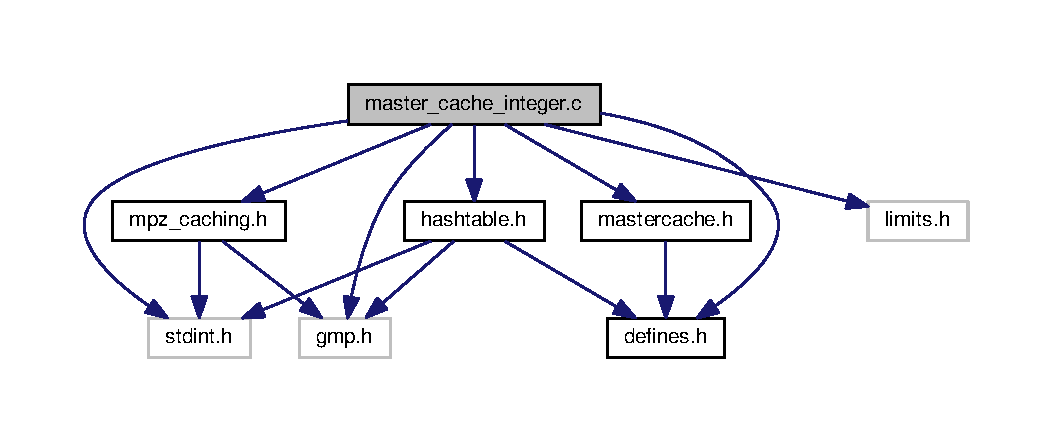
\includegraphics[width=350pt]{master__cache__integer_8c__incl}
\end{center}
\end{figure}
\subsection*{Functions}
\begin{DoxyCompactItemize}
\item 
\hyperlink{mastercache_8h_a113c03970467afb459ed5ae157d0a870}{cached\+Int} \hyperlink{master__cache__integer_8c_acf48c6c064be125bfc2e3daf62f10177}{direct\+\_\+add} (\hyperlink{mastercache_8h_a113c03970467afb459ed5ae157d0a870}{cached\+Int} val1, \hyperlink{mastercache_8h_a113c03970467afb459ed5ae157d0a870}{cached\+Int} val2)
\item 
\hyperlink{mastercache_8h_a113c03970467afb459ed5ae157d0a870}{cached\+Int} \hyperlink{master__cache__integer_8c_aa558a557fa5371fc35597dc52fd824e5}{direct\+\_\+mul} (\hyperlink{mastercache_8h_a113c03970467afb459ed5ae157d0a870}{cached\+Int} val1, \hyperlink{mastercache_8h_a113c03970467afb459ed5ae157d0a870}{cached\+Int} val2)
\item 
\hyperlink{mastercache_8h_a113c03970467afb459ed5ae157d0a870}{cached\+Int} \hyperlink{master__cache__integer_8c_a7cbe579aa33d35c4042fac942fed2070}{direct\+\_\+div} (\hyperlink{mastercache_8h_a113c03970467afb459ed5ae157d0a870}{cached\+Int} val1, \hyperlink{mastercache_8h_a113c03970467afb459ed5ae157d0a870}{cached\+Int} val2)
\item 
\hyperlink{mastercache_8h_a113c03970467afb459ed5ae157d0a870}{cached\+Int} \hyperlink{master__cache__integer_8c_abe0e4d423323534bba705a0e6fed30dc}{direct\+\_\+mod} (\hyperlink{mastercache_8h_a113c03970467afb459ed5ae157d0a870}{cached\+Int} val1, \hyperlink{mastercache_8h_a113c03970467afb459ed5ae157d0a870}{cached\+Int} val2)
\item 
\hyperlink{mastercache_8h_a113c03970467afb459ed5ae157d0a870}{cached\+Int} \hyperlink{master__cache__integer_8c_a663303ff03efc5249b8aa408ff5cce29}{direct\+\_\+gcd} (\hyperlink{mastercache_8h_a113c03970467afb459ed5ae157d0a870}{cached\+Int} val1, \hyperlink{mastercache_8h_a113c03970467afb459ed5ae157d0a870}{cached\+Int} val2)
\item 
\hyperlink{mastercache_8h_a113c03970467afb459ed5ae157d0a870}{cached\+Int} \hyperlink{master__cache__integer_8c_aae7d64a848078cd497869680dbca4780}{direct\+\_\+invert} (\hyperlink{mastercache_8h_a113c03970467afb459ed5ae157d0a870}{cached\+Int} val1, \hyperlink{mastercache_8h_a113c03970467afb459ed5ae157d0a870}{cached\+Int} val2)
\item 
void \hyperlink{master__cache__integer_8c_a66c8c57579e8806ff904aeb71d54ec44}{ext\+\_\+euclid} (\hyperlink{mastercache_8h_a113c03970467afb459ed5ae157d0a870}{cached\+Int} val1, \hyperlink{mastercache_8h_a113c03970467afb459ed5ae157d0a870}{cached\+Int} val2, \hyperlink{mastercache_8h_a113c03970467afb459ed5ae157d0a870}{cached\+Int} $\ast$d, \hyperlink{mastercache_8h_a113c03970467afb459ed5ae157d0a870}{cached\+Int} $\ast$s, \hyperlink{mastercache_8h_a113c03970467afb459ed5ae157d0a870}{cached\+Int} $\ast$t)
\item 
void \hyperlink{master__cache__integer_8c_a6095b13ce14cae93851e746599d8038e}{cached\+\_\+int\+\_\+init\+\_\+cache} (\hyperlink{structMasterCache}{Master\+Cache} $\ast$mstr, uint64\+\_\+t cachesize)
\begin{DoxyCompactList}\small\item\em function for master cache to initialize \end{DoxyCompactList}\item 
void \hyperlink{master__cache__integer_8c_a1f693b4093b62e1c70a866b4947cea00}{cached\+\_\+int\+\_\+clear\+\_\+cache} (\hyperlink{structMasterCache}{Master\+Cache} $\ast$mstr)
\begin{DoxyCompactList}\small\item\em function for master cache to clear all background data before free \end{DoxyCompactList}\item 
uint64\+\_\+t \hyperlink{master__cache__integer_8c_a8ad24c72fe1e1e7bcb71342763573276}{mpz\+\_\+cached\+\_\+int} (mpz\+\_\+t number)
\item 
void \hyperlink{master__cache__integer_8c_ac755a7c217e68e03bac95bda3c12e2a7}{cached\+\_\+int\+\_\+mpz} (\hyperlink{mastercache_8h_a113c03970467afb459ed5ae157d0a870}{cached\+Int} id, mpz\+\_\+t number)
\item 
\hyperlink{mastercache_8h_a113c03970467afb459ed5ae157d0a870}{cached\+Int} \hyperlink{master__cache__integer_8c_a2e8ed43761ae3945335b89102db422fd}{cached\+\_\+int\+\_\+set} (\hyperlink{structMasterCache}{Master\+Cache} $\ast$mstr, mpz\+\_\+t number)
\begin{DoxyCompactList}\small\item\em function for master cache to set a mpz\+\_\+t and get back an id \end{DoxyCompactList}\item 
void \hyperlink{master__cache__integer_8c_a70e68c14bd00b07597b31dba34aba997}{cached\+\_\+int\+\_\+get} (\hyperlink{structMasterCache}{Master\+Cache} $\ast$mstr, \hyperlink{mastercache_8h_a113c03970467afb459ed5ae157d0a870}{cached\+Int} id, mpz\+\_\+t number)
\begin{DoxyCompactList}\small\item\em function for master cache to get a previously cached mpz\+\_\+t from an id \end{DoxyCompactList}\item 
double \hyperlink{master__cache__integer_8c_af0c42f55a0674b42df4ce45322c33198}{cached\+\_\+int\+\_\+get\+\_\+d} (\hyperlink{structMasterCache}{Master\+Cache} $\ast$mstr, \hyperlink{mastercache_8h_a113c03970467afb459ed5ae157d0a870}{cached\+Int} id)
\begin{DoxyCompactList}\small\item\em function for master cache to get a previously cached mpz\+\_\+t as double from an id \end{DoxyCompactList}\item 
\hyperlink{mastercache_8h_a113c03970467afb459ed5ae157d0a870}{cached\+Int} \hyperlink{master__cache__integer_8c_a2c77389b27a3a9c47f580cc52b6bbe62}{cached\+\_\+int\+\_\+add} (\hyperlink{structMasterCache}{Master\+Cache} $\ast$mstr, \hyperlink{mastercache_8h_a113c03970467afb459ed5ae157d0a870}{cached\+Int} val1, \hyperlink{mastercache_8h_a113c03970467afb459ed5ae157d0a870}{cached\+Int} val2)
\begin{DoxyCompactList}\small\item\em function for master cache to add two cached values and cache the result if large. \end{DoxyCompactList}\item 
\hyperlink{mastercache_8h_a113c03970467afb459ed5ae157d0a870}{cached\+Int} \hyperlink{master__cache__integer_8c_af3fa99a34d3f8f474ca5cb1caf45b0dc}{cached\+\_\+int\+\_\+sub} (\hyperlink{structMasterCache}{Master\+Cache} $\ast$mstr, \hyperlink{mastercache_8h_a113c03970467afb459ed5ae157d0a870}{cached\+Int} val1, \hyperlink{mastercache_8h_a113c03970467afb459ed5ae157d0a870}{cached\+Int} val2)
\begin{DoxyCompactList}\small\item\em function for master cache to subtract two cached values and cache the result if large. \end{DoxyCompactList}\item 
\hyperlink{mastercache_8h_a113c03970467afb459ed5ae157d0a870}{cached\+Int} \hyperlink{master__cache__integer_8c_a418f697aefb1a082369940b69ef21758}{cached\+\_\+int\+\_\+mul} (\hyperlink{structMasterCache}{Master\+Cache} $\ast$mstr, \hyperlink{mastercache_8h_a113c03970467afb459ed5ae157d0a870}{cached\+Int} val1, \hyperlink{mastercache_8h_a113c03970467afb459ed5ae157d0a870}{cached\+Int} val2)
\begin{DoxyCompactList}\small\item\em function for master cache to multiply two cached values and cache the result if large. \end{DoxyCompactList}\item 
\hyperlink{mastercache_8h_a113c03970467afb459ed5ae157d0a870}{cached\+Int} \hyperlink{master__cache__integer_8c_a65de9b96c7568d2a4bc8a6a05749be04}{cached\+\_\+int\+\_\+tdiv} (\hyperlink{structMasterCache}{Master\+Cache} $\ast$mstr, \hyperlink{mastercache_8h_a113c03970467afb459ed5ae157d0a870}{cached\+Int} divident, \hyperlink{mastercache_8h_a113c03970467afb459ed5ae157d0a870}{cached\+Int} divisor, \hyperlink{mastercache_8h_a113c03970467afb459ed5ae157d0a870}{cached\+Int} $\ast$rest)
\begin{DoxyCompactList}\small\item\em function for master cache to divide two cached values and cache the result if large. \end{DoxyCompactList}\item 
\hyperlink{mastercache_8h_a113c03970467afb459ed5ae157d0a870}{cached\+Int} \hyperlink{master__cache__integer_8c_ac95bf4ec8ac8cdfc09f81dc6ab3f7954}{cached\+\_\+int\+\_\+mod} (\hyperlink{structMasterCache}{Master\+Cache} $\ast$mstr, \hyperlink{mastercache_8h_a113c03970467afb459ed5ae157d0a870}{cached\+Int} number, \hyperlink{mastercache_8h_a113c03970467afb459ed5ae157d0a870}{cached\+Int} n)
\begin{DoxyCompactList}\small\item\em function for master cache to calculate the modulo of two cached values and cache the result if large. \end{DoxyCompactList}\item 
\hyperlink{mastercache_8h_a113c03970467afb459ed5ae157d0a870}{cached\+Int} \hyperlink{master__cache__integer_8c_aee6e62d1fc9500706bd768db8e2a5af3}{cached\+\_\+int\+\_\+gcd} (\hyperlink{structMasterCache}{Master\+Cache} $\ast$mstr, \hyperlink{mastercache_8h_a113c03970467afb459ed5ae157d0a870}{cached\+Int} val1, \hyperlink{mastercache_8h_a113c03970467afb459ed5ae157d0a870}{cached\+Int} val2)
\begin{DoxyCompactList}\small\item\em function for master cache to calculate the greatest common divisor of two cached values and cache the result if large. \end{DoxyCompactList}\item 
int \hyperlink{master__cache__integer_8c_aaabedd43537e5425aebea90933ccaa75}{cached\+\_\+int\+\_\+invert} (\hyperlink{structMasterCache}{Master\+Cache} $\ast$mstr, \hyperlink{mastercache_8h_a113c03970467afb459ed5ae157d0a870}{cached\+Int} val1, \hyperlink{mastercache_8h_a113c03970467afb459ed5ae157d0a870}{cached\+Int} val2, \hyperlink{mastercache_8h_a113c03970467afb459ed5ae157d0a870}{cached\+Int} $\ast$result)
\begin{DoxyCompactList}\small\item\em function for master cache to calculate the inverse of a cached value mod n and cache the result if large. \end{DoxyCompactList}\end{DoxyCompactItemize}


\subsection{Detailed Description}
Master Cache functions for caching Integer operations in gmp. 

\begin{DoxyAuthor}{Author}
Sandra Hicks 
\end{DoxyAuthor}


\subsection{Function Documentation}
\index{master\+\_\+cache\+\_\+integer.\+c@{master\+\_\+cache\+\_\+integer.\+c}!cached\+\_\+int\+\_\+add@{cached\+\_\+int\+\_\+add}}
\index{cached\+\_\+int\+\_\+add@{cached\+\_\+int\+\_\+add}!master\+\_\+cache\+\_\+integer.\+c@{master\+\_\+cache\+\_\+integer.\+c}}
\subsubsection[{\texorpdfstring{cached\+\_\+int\+\_\+add(\+Master\+Cache $\ast$mstr, cached\+Int val1, cached\+Int val2)}{cached_int_add(MasterCache *mstr, cachedInt val1, cachedInt val2)}}]{\setlength{\rightskip}{0pt plus 5cm}{\bf cached\+Int} cached\+\_\+int\+\_\+add (
\begin{DoxyParamCaption}
\item[{{\bf Master\+Cache} $\ast$}]{mstr, }
\item[{{\bf cached\+Int}}]{val1, }
\item[{{\bf cached\+Int}}]{val2}
\end{DoxyParamCaption}
)}\hypertarget{master__cache__integer_8c_a2c77389b27a3a9c47f580cc52b6bbe62}{}\label{master__cache__integer_8c_a2c77389b27a3a9c47f580cc52b6bbe62}


function for master cache to add two cached values and cache the result if large. 


\begin{DoxyParams}{Parameters}
{\em mstr} & \hyperlink{structMasterCache}{Master\+Cache} pointer \\
\hline
{\em val1} & id of the first operand \\
\hline
{\em val2} & id of the second operand \\
\hline
\end{DoxyParams}
\begin{DoxyReturn}{Returns}
cached\+Int returns caching id or result for addtion 
\end{DoxyReturn}
\index{master\+\_\+cache\+\_\+integer.\+c@{master\+\_\+cache\+\_\+integer.\+c}!cached\+\_\+int\+\_\+clear\+\_\+cache@{cached\+\_\+int\+\_\+clear\+\_\+cache}}
\index{cached\+\_\+int\+\_\+clear\+\_\+cache@{cached\+\_\+int\+\_\+clear\+\_\+cache}!master\+\_\+cache\+\_\+integer.\+c@{master\+\_\+cache\+\_\+integer.\+c}}
\subsubsection[{\texorpdfstring{cached\+\_\+int\+\_\+clear\+\_\+cache(\+Master\+Cache $\ast$mstr)}{cached_int_clear_cache(MasterCache *mstr)}}]{\setlength{\rightskip}{0pt plus 5cm}void cached\+\_\+int\+\_\+clear\+\_\+cache (
\begin{DoxyParamCaption}
\item[{{\bf Master\+Cache} $\ast$}]{mstr}
\end{DoxyParamCaption}
)}\hypertarget{master__cache__integer_8c_a1f693b4093b62e1c70a866b4947cea00}{}\label{master__cache__integer_8c_a1f693b4093b62e1c70a866b4947cea00}


function for master cache to clear all background data before free 


\begin{DoxyParams}{Parameters}
{\em mstr} & \hyperlink{structMasterCache}{Master\+Cache} pointer \\
\hline
\end{DoxyParams}
\index{master\+\_\+cache\+\_\+integer.\+c@{master\+\_\+cache\+\_\+integer.\+c}!cached\+\_\+int\+\_\+gcd@{cached\+\_\+int\+\_\+gcd}}
\index{cached\+\_\+int\+\_\+gcd@{cached\+\_\+int\+\_\+gcd}!master\+\_\+cache\+\_\+integer.\+c@{master\+\_\+cache\+\_\+integer.\+c}}
\subsubsection[{\texorpdfstring{cached\+\_\+int\+\_\+gcd(\+Master\+Cache $\ast$mstr, cached\+Int val1, cached\+Int val2)}{cached_int_gcd(MasterCache *mstr, cachedInt val1, cachedInt val2)}}]{\setlength{\rightskip}{0pt plus 5cm}{\bf cached\+Int} cached\+\_\+int\+\_\+gcd (
\begin{DoxyParamCaption}
\item[{{\bf Master\+Cache} $\ast$}]{mstr, }
\item[{{\bf cached\+Int}}]{val1, }
\item[{{\bf cached\+Int}}]{val2}
\end{DoxyParamCaption}
)}\hypertarget{master__cache__integer_8c_aee6e62d1fc9500706bd768db8e2a5af3}{}\label{master__cache__integer_8c_aee6e62d1fc9500706bd768db8e2a5af3}


function for master cache to calculate the greatest common divisor of two cached values and cache the result if large. 


\begin{DoxyParams}{Parameters}
{\em mstr} & \hyperlink{structMasterCache}{Master\+Cache} pointer \\
\hline
{\em val1} & id of the first operand \\
\hline
{\em val2} & id of the second operand \\
\hline
\end{DoxyParams}
\begin{DoxyReturn}{Returns}
cached\+Int returns caching id or result for gcd 
\end{DoxyReturn}
\index{master\+\_\+cache\+\_\+integer.\+c@{master\+\_\+cache\+\_\+integer.\+c}!cached\+\_\+int\+\_\+get@{cached\+\_\+int\+\_\+get}}
\index{cached\+\_\+int\+\_\+get@{cached\+\_\+int\+\_\+get}!master\+\_\+cache\+\_\+integer.\+c@{master\+\_\+cache\+\_\+integer.\+c}}
\subsubsection[{\texorpdfstring{cached\+\_\+int\+\_\+get(\+Master\+Cache $\ast$mstr, cached\+Int id, mpz\+\_\+t number)}{cached_int_get(MasterCache *mstr, cachedInt id, mpz_t number)}}]{\setlength{\rightskip}{0pt plus 5cm}void cached\+\_\+int\+\_\+get (
\begin{DoxyParamCaption}
\item[{{\bf Master\+Cache} $\ast$}]{mstr, }
\item[{{\bf cached\+Int}}]{id, }
\item[{mpz\+\_\+t}]{number}
\end{DoxyParamCaption}
)}\hypertarget{master__cache__integer_8c_a70e68c14bd00b07597b31dba34aba997}{}\label{master__cache__integer_8c_a70e68c14bd00b07597b31dba34aba997}


function for master cache to get a previously cached mpz\+\_\+t from an id 


\begin{DoxyParams}{Parameters}
{\em mstr} & \hyperlink{structMasterCache}{Master\+Cache} pointer \\
\hline
{\em id} & cached\+Int id that was cached \\
\hline
{\em number} & mpz\+\_\+t number to set \\
\hline
\end{DoxyParams}
\index{master\+\_\+cache\+\_\+integer.\+c@{master\+\_\+cache\+\_\+integer.\+c}!cached\+\_\+int\+\_\+get\+\_\+d@{cached\+\_\+int\+\_\+get\+\_\+d}}
\index{cached\+\_\+int\+\_\+get\+\_\+d@{cached\+\_\+int\+\_\+get\+\_\+d}!master\+\_\+cache\+\_\+integer.\+c@{master\+\_\+cache\+\_\+integer.\+c}}
\subsubsection[{\texorpdfstring{cached\+\_\+int\+\_\+get\+\_\+d(\+Master\+Cache $\ast$mstr, cached\+Int id)}{cached_int_get_d(MasterCache *mstr, cachedInt id)}}]{\setlength{\rightskip}{0pt plus 5cm}double cached\+\_\+int\+\_\+get\+\_\+d (
\begin{DoxyParamCaption}
\item[{{\bf Master\+Cache} $\ast$}]{mstr, }
\item[{{\bf cached\+Int}}]{id}
\end{DoxyParamCaption}
)}\hypertarget{master__cache__integer_8c_af0c42f55a0674b42df4ce45322c33198}{}\label{master__cache__integer_8c_af0c42f55a0674b42df4ce45322c33198}


function for master cache to get a previously cached mpz\+\_\+t as double from an id 


\begin{DoxyParams}{Parameters}
{\em mstr} & \hyperlink{structMasterCache}{Master\+Cache} pointer \\
\hline
{\em id} & cached\+Int id that was cached \\
\hline
\end{DoxyParams}
\begin{DoxyReturn}{Returns}
double the double representation of the mpz cached with id 
\end{DoxyReturn}
\index{master\+\_\+cache\+\_\+integer.\+c@{master\+\_\+cache\+\_\+integer.\+c}!cached\+\_\+int\+\_\+init\+\_\+cache@{cached\+\_\+int\+\_\+init\+\_\+cache}}
\index{cached\+\_\+int\+\_\+init\+\_\+cache@{cached\+\_\+int\+\_\+init\+\_\+cache}!master\+\_\+cache\+\_\+integer.\+c@{master\+\_\+cache\+\_\+integer.\+c}}
\subsubsection[{\texorpdfstring{cached\+\_\+int\+\_\+init\+\_\+cache(\+Master\+Cache $\ast$mstr, uint64\+\_\+t cachesize)}{cached_int_init_cache(MasterCache *mstr, uint64_t cachesize)}}]{\setlength{\rightskip}{0pt plus 5cm}void cached\+\_\+int\+\_\+init\+\_\+cache (
\begin{DoxyParamCaption}
\item[{{\bf Master\+Cache} $\ast$}]{mstr, }
\item[{uint64\+\_\+t}]{cachesize}
\end{DoxyParamCaption}
)}\hypertarget{master__cache__integer_8c_a6095b13ce14cae93851e746599d8038e}{}\label{master__cache__integer_8c_a6095b13ce14cae93851e746599d8038e}


function for master cache to initialize 


\begin{DoxyParams}{Parameters}
{\em mstr} & \hyperlink{structMasterCache}{Master\+Cache} pointer \\
\hline
{\em cachesize} & uint64\+\_\+t with user defined size of the cache \\
\hline
\end{DoxyParams}
\index{master\+\_\+cache\+\_\+integer.\+c@{master\+\_\+cache\+\_\+integer.\+c}!cached\+\_\+int\+\_\+invert@{cached\+\_\+int\+\_\+invert}}
\index{cached\+\_\+int\+\_\+invert@{cached\+\_\+int\+\_\+invert}!master\+\_\+cache\+\_\+integer.\+c@{master\+\_\+cache\+\_\+integer.\+c}}
\subsubsection[{\texorpdfstring{cached\+\_\+int\+\_\+invert(\+Master\+Cache $\ast$mstr, cached\+Int val1, cached\+Int val2, cached\+Int $\ast$result)}{cached_int_invert(MasterCache *mstr, cachedInt val1, cachedInt val2, cachedInt *result)}}]{\setlength{\rightskip}{0pt plus 5cm}int cached\+\_\+int\+\_\+invert (
\begin{DoxyParamCaption}
\item[{{\bf Master\+Cache} $\ast$}]{mstr, }
\item[{{\bf cached\+Int}}]{val1, }
\item[{{\bf cached\+Int}}]{val2, }
\item[{{\bf cached\+Int} $\ast$}]{result}
\end{DoxyParamCaption}
)}\hypertarget{master__cache__integer_8c_aaabedd43537e5425aebea90933ccaa75}{}\label{master__cache__integer_8c_aaabedd43537e5425aebea90933ccaa75}


function for master cache to calculate the inverse of a cached value mod n and cache the result if large. 


\begin{DoxyParams}{Parameters}
{\em mstr} & \hyperlink{structMasterCache}{Master\+Cache} pointer \\
\hline
{\em val1} & id of the first operand \\
\hline
{\em val2} & id of the second operand \\
\hline
{\em result} & pointer for returning result \\
\hline
\end{DoxyParams}
\begin{DoxyReturn}{Returns}
int returns 0 if inverse does not exists, 1 if result is defined 
\end{DoxyReturn}
\index{master\+\_\+cache\+\_\+integer.\+c@{master\+\_\+cache\+\_\+integer.\+c}!cached\+\_\+int\+\_\+mod@{cached\+\_\+int\+\_\+mod}}
\index{cached\+\_\+int\+\_\+mod@{cached\+\_\+int\+\_\+mod}!master\+\_\+cache\+\_\+integer.\+c@{master\+\_\+cache\+\_\+integer.\+c}}
\subsubsection[{\texorpdfstring{cached\+\_\+int\+\_\+mod(\+Master\+Cache $\ast$mstr, cached\+Int number, cached\+Int n)}{cached_int_mod(MasterCache *mstr, cachedInt number, cachedInt n)}}]{\setlength{\rightskip}{0pt plus 5cm}{\bf cached\+Int} cached\+\_\+int\+\_\+mod (
\begin{DoxyParamCaption}
\item[{{\bf Master\+Cache} $\ast$}]{mstr, }
\item[{{\bf cached\+Int}}]{number, }
\item[{{\bf cached\+Int}}]{n}
\end{DoxyParamCaption}
)}\hypertarget{master__cache__integer_8c_ac95bf4ec8ac8cdfc09f81dc6ab3f7954}{}\label{master__cache__integer_8c_ac95bf4ec8ac8cdfc09f81dc6ab3f7954}


function for master cache to calculate the modulo of two cached values and cache the result if large. 


\begin{DoxyParams}{Parameters}
{\em mstr} & \hyperlink{structMasterCache}{Master\+Cache} pointer \\
\hline
{\em number} & id of the first operand \\
\hline
{\em n} & id of the second operand \\
\hline
\end{DoxyParams}
\begin{DoxyReturn}{Returns}
cached\+Int returns caching id or result for mod 
\end{DoxyReturn}
\index{master\+\_\+cache\+\_\+integer.\+c@{master\+\_\+cache\+\_\+integer.\+c}!cached\+\_\+int\+\_\+mpz@{cached\+\_\+int\+\_\+mpz}}
\index{cached\+\_\+int\+\_\+mpz@{cached\+\_\+int\+\_\+mpz}!master\+\_\+cache\+\_\+integer.\+c@{master\+\_\+cache\+\_\+integer.\+c}}
\subsubsection[{\texorpdfstring{cached\+\_\+int\+\_\+mpz(cached\+Int id, mpz\+\_\+t number)}{cached_int_mpz(cachedInt id, mpz_t number)}}]{\setlength{\rightskip}{0pt plus 5cm}void cached\+\_\+int\+\_\+mpz (
\begin{DoxyParamCaption}
\item[{{\bf cached\+Int}}]{id, }
\item[{mpz\+\_\+t}]{number}
\end{DoxyParamCaption}
)}\hypertarget{master__cache__integer_8c_ac755a7c217e68e03bac95bda3c12e2a7}{}\label{master__cache__integer_8c_ac755a7c217e68e03bac95bda3c12e2a7}
(for internal use only!) 
\begin{DoxyParams}{Parameters}
{\em id} & \\
\hline
{\em number} & \\
\hline
\end{DoxyParams}
\index{master\+\_\+cache\+\_\+integer.\+c@{master\+\_\+cache\+\_\+integer.\+c}!cached\+\_\+int\+\_\+mul@{cached\+\_\+int\+\_\+mul}}
\index{cached\+\_\+int\+\_\+mul@{cached\+\_\+int\+\_\+mul}!master\+\_\+cache\+\_\+integer.\+c@{master\+\_\+cache\+\_\+integer.\+c}}
\subsubsection[{\texorpdfstring{cached\+\_\+int\+\_\+mul(\+Master\+Cache $\ast$mstr, cached\+Int val1, cached\+Int val2)}{cached_int_mul(MasterCache *mstr, cachedInt val1, cachedInt val2)}}]{\setlength{\rightskip}{0pt plus 5cm}{\bf cached\+Int} cached\+\_\+int\+\_\+mul (
\begin{DoxyParamCaption}
\item[{{\bf Master\+Cache} $\ast$}]{mstr, }
\item[{{\bf cached\+Int}}]{val1, }
\item[{{\bf cached\+Int}}]{val2}
\end{DoxyParamCaption}
)}\hypertarget{master__cache__integer_8c_a418f697aefb1a082369940b69ef21758}{}\label{master__cache__integer_8c_a418f697aefb1a082369940b69ef21758}


function for master cache to multiply two cached values and cache the result if large. 


\begin{DoxyParams}{Parameters}
{\em mstr} & \hyperlink{structMasterCache}{Master\+Cache} pointer \\
\hline
{\em val1} & id of the first operand \\
\hline
{\em val2} & id of the second operand \\
\hline
\end{DoxyParams}
\begin{DoxyReturn}{Returns}
cached\+Int returns caching id or result for multiplication 
\end{DoxyReturn}
\index{master\+\_\+cache\+\_\+integer.\+c@{master\+\_\+cache\+\_\+integer.\+c}!cached\+\_\+int\+\_\+set@{cached\+\_\+int\+\_\+set}}
\index{cached\+\_\+int\+\_\+set@{cached\+\_\+int\+\_\+set}!master\+\_\+cache\+\_\+integer.\+c@{master\+\_\+cache\+\_\+integer.\+c}}
\subsubsection[{\texorpdfstring{cached\+\_\+int\+\_\+set(\+Master\+Cache $\ast$mstr, mpz\+\_\+t number)}{cached_int_set(MasterCache *mstr, mpz_t number)}}]{\setlength{\rightskip}{0pt plus 5cm}{\bf cached\+Int} cached\+\_\+int\+\_\+set (
\begin{DoxyParamCaption}
\item[{{\bf Master\+Cache} $\ast$}]{mstr, }
\item[{mpz\+\_\+t}]{number}
\end{DoxyParamCaption}
)}\hypertarget{master__cache__integer_8c_a2e8ed43761ae3945335b89102db422fd}{}\label{master__cache__integer_8c_a2e8ed43761ae3945335b89102db422fd}


function for master cache to set a mpz\+\_\+t and get back an id 


\begin{DoxyParams}{Parameters}
{\em mstr} & \hyperlink{structMasterCache}{Master\+Cache} pointer \\
\hline
{\em number} & number to cache \\
\hline
\end{DoxyParams}
\begin{DoxyReturn}{Returns}
cached\+Int id for cached mpz\+\_\+t 
\end{DoxyReturn}
\index{master\+\_\+cache\+\_\+integer.\+c@{master\+\_\+cache\+\_\+integer.\+c}!cached\+\_\+int\+\_\+sub@{cached\+\_\+int\+\_\+sub}}
\index{cached\+\_\+int\+\_\+sub@{cached\+\_\+int\+\_\+sub}!master\+\_\+cache\+\_\+integer.\+c@{master\+\_\+cache\+\_\+integer.\+c}}
\subsubsection[{\texorpdfstring{cached\+\_\+int\+\_\+sub(\+Master\+Cache $\ast$mstr, cached\+Int val1, cached\+Int val2)}{cached_int_sub(MasterCache *mstr, cachedInt val1, cachedInt val2)}}]{\setlength{\rightskip}{0pt plus 5cm}{\bf cached\+Int} cached\+\_\+int\+\_\+sub (
\begin{DoxyParamCaption}
\item[{{\bf Master\+Cache} $\ast$}]{mstr, }
\item[{{\bf cached\+Int}}]{val1, }
\item[{{\bf cached\+Int}}]{val2}
\end{DoxyParamCaption}
)}\hypertarget{master__cache__integer_8c_af3fa99a34d3f8f474ca5cb1caf45b0dc}{}\label{master__cache__integer_8c_af3fa99a34d3f8f474ca5cb1caf45b0dc}


function for master cache to subtract two cached values and cache the result if large. 


\begin{DoxyParams}{Parameters}
{\em mstr} & \hyperlink{structMasterCache}{Master\+Cache} pointer \\
\hline
{\em val1} & id of the first operand \\
\hline
{\em val2} & id of the second operand \\
\hline
\end{DoxyParams}
\begin{DoxyReturn}{Returns}
cached\+Int returns caching id or result for subtraction 
\end{DoxyReturn}
\index{master\+\_\+cache\+\_\+integer.\+c@{master\+\_\+cache\+\_\+integer.\+c}!cached\+\_\+int\+\_\+tdiv@{cached\+\_\+int\+\_\+tdiv}}
\index{cached\+\_\+int\+\_\+tdiv@{cached\+\_\+int\+\_\+tdiv}!master\+\_\+cache\+\_\+integer.\+c@{master\+\_\+cache\+\_\+integer.\+c}}
\subsubsection[{\texorpdfstring{cached\+\_\+int\+\_\+tdiv(\+Master\+Cache $\ast$mstr, cached\+Int divident, cached\+Int divisor, cached\+Int $\ast$rest)}{cached_int_tdiv(MasterCache *mstr, cachedInt divident, cachedInt divisor, cachedInt *rest)}}]{\setlength{\rightskip}{0pt plus 5cm}{\bf cached\+Int} cached\+\_\+int\+\_\+tdiv (
\begin{DoxyParamCaption}
\item[{{\bf Master\+Cache} $\ast$}]{mstr, }
\item[{{\bf cached\+Int}}]{divident, }
\item[{{\bf cached\+Int}}]{divisor, }
\item[{{\bf cached\+Int} $\ast$}]{rest}
\end{DoxyParamCaption}
)}\hypertarget{master__cache__integer_8c_a65de9b96c7568d2a4bc8a6a05749be04}{}\label{master__cache__integer_8c_a65de9b96c7568d2a4bc8a6a05749be04}


function for master cache to divide two cached values and cache the result if large. 


\begin{DoxyParams}{Parameters}
{\em mstr} & \hyperlink{structMasterCache}{Master\+Cache} pointer \\
\hline
{\em divident} & id of the first operand \\
\hline
{\em divisor} & id of the second operand \\
\hline
{\em rest} & pointer to id for rest of division \\
\hline
\end{DoxyParams}
\begin{DoxyReturn}{Returns}
cached\+Int returns caching id or result for division 
\end{DoxyReturn}
\index{master\+\_\+cache\+\_\+integer.\+c@{master\+\_\+cache\+\_\+integer.\+c}!direct\+\_\+add@{direct\+\_\+add}}
\index{direct\+\_\+add@{direct\+\_\+add}!master\+\_\+cache\+\_\+integer.\+c@{master\+\_\+cache\+\_\+integer.\+c}}
\subsubsection[{\texorpdfstring{direct\+\_\+add(cached\+Int val1, cached\+Int val2)}{direct_add(cachedInt val1, cachedInt val2)}}]{\setlength{\rightskip}{0pt plus 5cm}{\bf cached\+Int} direct\+\_\+add (
\begin{DoxyParamCaption}
\item[{{\bf cached\+Int}}]{val1, }
\item[{{\bf cached\+Int}}]{val2}
\end{DoxyParamCaption}
)}\hypertarget{master__cache__integer_8c_acf48c6c064be125bfc2e3daf62f10177}{}\label{master__cache__integer_8c_acf48c6c064be125bfc2e3daf62f10177}
(for internal use only!) 
\begin{DoxyParams}{Parameters}
{\em val1} & \\
\hline
{\em val2} & \\
\hline
\end{DoxyParams}
\begin{DoxyReturn}{Returns}

\end{DoxyReturn}
\index{master\+\_\+cache\+\_\+integer.\+c@{master\+\_\+cache\+\_\+integer.\+c}!direct\+\_\+div@{direct\+\_\+div}}
\index{direct\+\_\+div@{direct\+\_\+div}!master\+\_\+cache\+\_\+integer.\+c@{master\+\_\+cache\+\_\+integer.\+c}}
\subsubsection[{\texorpdfstring{direct\+\_\+div(cached\+Int val1, cached\+Int val2)}{direct_div(cachedInt val1, cachedInt val2)}}]{\setlength{\rightskip}{0pt plus 5cm}{\bf cached\+Int} direct\+\_\+div (
\begin{DoxyParamCaption}
\item[{{\bf cached\+Int}}]{val1, }
\item[{{\bf cached\+Int}}]{val2}
\end{DoxyParamCaption}
)}\hypertarget{master__cache__integer_8c_a7cbe579aa33d35c4042fac942fed2070}{}\label{master__cache__integer_8c_a7cbe579aa33d35c4042fac942fed2070}
(for internal use only!) 
\begin{DoxyParams}{Parameters}
{\em val1} & \\
\hline
{\em val2} & \\
\hline
\end{DoxyParams}
\begin{DoxyReturn}{Returns}

\end{DoxyReturn}
\index{master\+\_\+cache\+\_\+integer.\+c@{master\+\_\+cache\+\_\+integer.\+c}!direct\+\_\+gcd@{direct\+\_\+gcd}}
\index{direct\+\_\+gcd@{direct\+\_\+gcd}!master\+\_\+cache\+\_\+integer.\+c@{master\+\_\+cache\+\_\+integer.\+c}}
\subsubsection[{\texorpdfstring{direct\+\_\+gcd(cached\+Int val1, cached\+Int val2)}{direct_gcd(cachedInt val1, cachedInt val2)}}]{\setlength{\rightskip}{0pt plus 5cm}{\bf cached\+Int} direct\+\_\+gcd (
\begin{DoxyParamCaption}
\item[{{\bf cached\+Int}}]{val1, }
\item[{{\bf cached\+Int}}]{val2}
\end{DoxyParamCaption}
)}\hypertarget{master__cache__integer_8c_a663303ff03efc5249b8aa408ff5cce29}{}\label{master__cache__integer_8c_a663303ff03efc5249b8aa408ff5cce29}
(for internal use only!) 
\begin{DoxyParams}{Parameters}
{\em val1} & \\
\hline
{\em val2} & \\
\hline
\end{DoxyParams}
\begin{DoxyReturn}{Returns}

\end{DoxyReturn}
\index{master\+\_\+cache\+\_\+integer.\+c@{master\+\_\+cache\+\_\+integer.\+c}!direct\+\_\+invert@{direct\+\_\+invert}}
\index{direct\+\_\+invert@{direct\+\_\+invert}!master\+\_\+cache\+\_\+integer.\+c@{master\+\_\+cache\+\_\+integer.\+c}}
\subsubsection[{\texorpdfstring{direct\+\_\+invert(cached\+Int val1, cached\+Int val2)}{direct_invert(cachedInt val1, cachedInt val2)}}]{\setlength{\rightskip}{0pt plus 5cm}{\bf cached\+Int} direct\+\_\+invert (
\begin{DoxyParamCaption}
\item[{{\bf cached\+Int}}]{val1, }
\item[{{\bf cached\+Int}}]{val2}
\end{DoxyParamCaption}
)}\hypertarget{master__cache__integer_8c_aae7d64a848078cd497869680dbca4780}{}\label{master__cache__integer_8c_aae7d64a848078cd497869680dbca4780}
(for internal use only!) 
\begin{DoxyParams}{Parameters}
{\em val1} & \\
\hline
{\em val2} & \\
\hline
\end{DoxyParams}
\begin{DoxyReturn}{Returns}

\end{DoxyReturn}
\index{master\+\_\+cache\+\_\+integer.\+c@{master\+\_\+cache\+\_\+integer.\+c}!direct\+\_\+mod@{direct\+\_\+mod}}
\index{direct\+\_\+mod@{direct\+\_\+mod}!master\+\_\+cache\+\_\+integer.\+c@{master\+\_\+cache\+\_\+integer.\+c}}
\subsubsection[{\texorpdfstring{direct\+\_\+mod(cached\+Int val1, cached\+Int val2)}{direct_mod(cachedInt val1, cachedInt val2)}}]{\setlength{\rightskip}{0pt plus 5cm}{\bf cached\+Int} direct\+\_\+mod (
\begin{DoxyParamCaption}
\item[{{\bf cached\+Int}}]{val1, }
\item[{{\bf cached\+Int}}]{val2}
\end{DoxyParamCaption}
)}\hypertarget{master__cache__integer_8c_abe0e4d423323534bba705a0e6fed30dc}{}\label{master__cache__integer_8c_abe0e4d423323534bba705a0e6fed30dc}
(for internal use only!) 
\begin{DoxyParams}{Parameters}
{\em val1} & \\
\hline
{\em val2} & \\
\hline
\end{DoxyParams}
\begin{DoxyReturn}{Returns}

\end{DoxyReturn}
\index{master\+\_\+cache\+\_\+integer.\+c@{master\+\_\+cache\+\_\+integer.\+c}!direct\+\_\+mul@{direct\+\_\+mul}}
\index{direct\+\_\+mul@{direct\+\_\+mul}!master\+\_\+cache\+\_\+integer.\+c@{master\+\_\+cache\+\_\+integer.\+c}}
\subsubsection[{\texorpdfstring{direct\+\_\+mul(cached\+Int val1, cached\+Int val2)}{direct_mul(cachedInt val1, cachedInt val2)}}]{\setlength{\rightskip}{0pt plus 5cm}{\bf cached\+Int} direct\+\_\+mul (
\begin{DoxyParamCaption}
\item[{{\bf cached\+Int}}]{val1, }
\item[{{\bf cached\+Int}}]{val2}
\end{DoxyParamCaption}
)}\hypertarget{master__cache__integer_8c_aa558a557fa5371fc35597dc52fd824e5}{}\label{master__cache__integer_8c_aa558a557fa5371fc35597dc52fd824e5}
(for internal use only!) 
\begin{DoxyParams}{Parameters}
{\em val1} & \\
\hline
{\em val2} & \\
\hline
\end{DoxyParams}
\begin{DoxyReturn}{Returns}

\end{DoxyReturn}
\index{master\+\_\+cache\+\_\+integer.\+c@{master\+\_\+cache\+\_\+integer.\+c}!ext\+\_\+euclid@{ext\+\_\+euclid}}
\index{ext\+\_\+euclid@{ext\+\_\+euclid}!master\+\_\+cache\+\_\+integer.\+c@{master\+\_\+cache\+\_\+integer.\+c}}
\subsubsection[{\texorpdfstring{ext\+\_\+euclid(cached\+Int val1, cached\+Int val2, cached\+Int $\ast$d, cached\+Int $\ast$s, cached\+Int $\ast$t)}{ext_euclid(cachedInt val1, cachedInt val2, cachedInt *d, cachedInt *s, cachedInt *t)}}]{\setlength{\rightskip}{0pt plus 5cm}void ext\+\_\+euclid (
\begin{DoxyParamCaption}
\item[{{\bf cached\+Int}}]{val1, }
\item[{{\bf cached\+Int}}]{val2, }
\item[{{\bf cached\+Int} $\ast$}]{d, }
\item[{{\bf cached\+Int} $\ast$}]{s, }
\item[{{\bf cached\+Int} $\ast$}]{t}
\end{DoxyParamCaption}
)}\hypertarget{master__cache__integer_8c_a66c8c57579e8806ff904aeb71d54ec44}{}\label{master__cache__integer_8c_a66c8c57579e8806ff904aeb71d54ec44}
(for internal use only!) 
\begin{DoxyParams}{Parameters}
{\em val1} & \\
\hline
{\em val2} & \\
\hline
{\em d} & \\
\hline
{\em s} & \\
\hline
{\em t} & \\
\hline
\end{DoxyParams}
\index{master\+\_\+cache\+\_\+integer.\+c@{master\+\_\+cache\+\_\+integer.\+c}!mpz\+\_\+cached\+\_\+int@{mpz\+\_\+cached\+\_\+int}}
\index{mpz\+\_\+cached\+\_\+int@{mpz\+\_\+cached\+\_\+int}!master\+\_\+cache\+\_\+integer.\+c@{master\+\_\+cache\+\_\+integer.\+c}}
\subsubsection[{\texorpdfstring{mpz\+\_\+cached\+\_\+int(mpz\+\_\+t number)}{mpz_cached_int(mpz_t number)}}]{\setlength{\rightskip}{0pt plus 5cm}uint64\+\_\+t mpz\+\_\+cached\+\_\+int (
\begin{DoxyParamCaption}
\item[{mpz\+\_\+t}]{number}
\end{DoxyParamCaption}
)}\hypertarget{master__cache__integer_8c_a8ad24c72fe1e1e7bcb71342763573276}{}\label{master__cache__integer_8c_a8ad24c72fe1e1e7bcb71342763573276}
(for internal use only!) 
\begin{DoxyParams}{Parameters}
{\em number} & \\
\hline
\end{DoxyParams}
\begin{DoxyReturn}{Returns}

\end{DoxyReturn}

\hypertarget{master__cache__integer_8h}{}\section{master\+\_\+cache\+\_\+integer.\+h File Reference}
\label{master__cache__integer_8h}\index{master\+\_\+cache\+\_\+integer.\+h@{master\+\_\+cache\+\_\+integer.\+h}}


header for Master Cache functions for caching Integer operations in gmp  


{\ttfamily \#include \char`\"{}mastercache.\+h\char`\"{}}\\*
Include dependency graph for master\+\_\+cache\+\_\+integer.\+h\+:\nopagebreak
\begin{figure}[H]
\begin{center}
\leavevmode
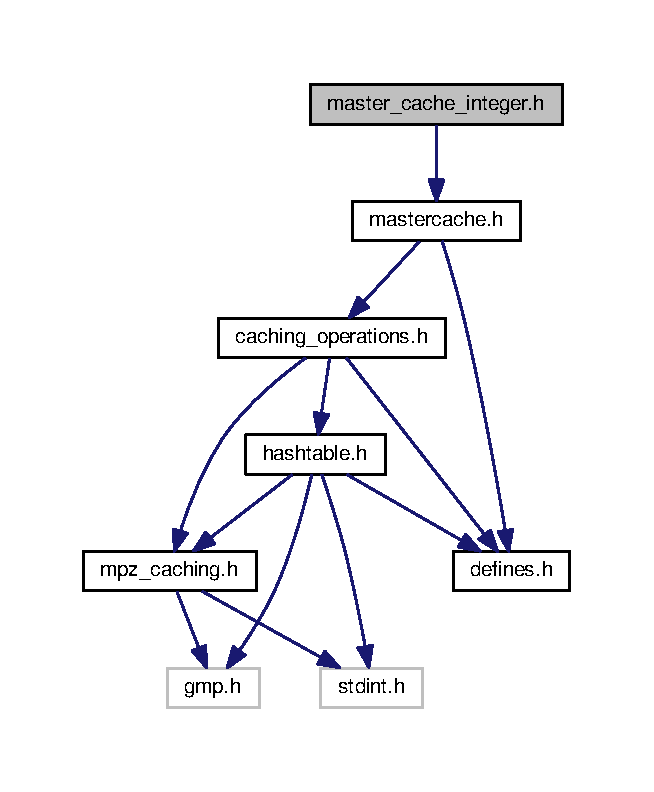
\includegraphics[width=314pt]{master__cache__integer_8h__incl}
\end{center}
\end{figure}
This graph shows which files directly or indirectly include this file\+:\nopagebreak
\begin{figure}[H]
\begin{center}
\leavevmode
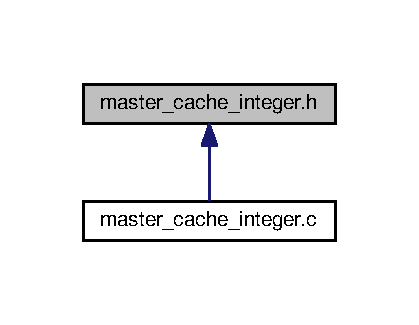
\includegraphics[width=201pt]{master__cache__integer_8h__dep__incl}
\end{center}
\end{figure}
\subsection*{Functions}
\begin{DoxyCompactItemize}
\item 
void \hyperlink{master__cache__integer_8h_a6095b13ce14cae93851e746599d8038e}{cached\+\_\+int\+\_\+init\+\_\+cache} (\hyperlink{structMasterCache}{Master\+Cache} $\ast$mstr, uint64\+\_\+t cachesize)
\begin{DoxyCompactList}\small\item\em function for master cache to initialize \end{DoxyCompactList}\item 
void \hyperlink{master__cache__integer_8h_a1f693b4093b62e1c70a866b4947cea00}{cached\+\_\+int\+\_\+clear\+\_\+cache} (\hyperlink{structMasterCache}{Master\+Cache} $\ast$mstr)
\begin{DoxyCompactList}\small\item\em function for master cache to clear all background data before free \end{DoxyCompactList}\item 
\hyperlink{mastercache_8h_a113c03970467afb459ed5ae157d0a870}{cached\+Int} \hyperlink{master__cache__integer_8h_a2e8ed43761ae3945335b89102db422fd}{cached\+\_\+int\+\_\+set} (\hyperlink{structMasterCache}{Master\+Cache} $\ast$mstr, mpz\+\_\+t number)
\begin{DoxyCompactList}\small\item\em function for master cache to set a mpz\+\_\+t and get back an id \end{DoxyCompactList}\item 
void \hyperlink{master__cache__integer_8h_a70e68c14bd00b07597b31dba34aba997}{cached\+\_\+int\+\_\+get} (\hyperlink{structMasterCache}{Master\+Cache} $\ast$mstr, \hyperlink{mastercache_8h_a113c03970467afb459ed5ae157d0a870}{cached\+Int} id, mpz\+\_\+t number)
\begin{DoxyCompactList}\small\item\em function for master cache to get a previously cached mpz\+\_\+t from an id \end{DoxyCompactList}\item 
double \hyperlink{master__cache__integer_8h_af0c42f55a0674b42df4ce45322c33198}{cached\+\_\+int\+\_\+get\+\_\+d} (\hyperlink{structMasterCache}{Master\+Cache} $\ast$mstr, \hyperlink{mastercache_8h_a113c03970467afb459ed5ae157d0a870}{cached\+Int} id)
\begin{DoxyCompactList}\small\item\em function for master cache to get a previously cached mpz\+\_\+t as double from an id \end{DoxyCompactList}\item 
void \hyperlink{master__cache__integer_8h_ac755a7c217e68e03bac95bda3c12e2a7}{cached\+\_\+int\+\_\+mpz} (\hyperlink{mastercache_8h_a113c03970467afb459ed5ae157d0a870}{cached\+Int} id, mpz\+\_\+t number)
\item 
uint64\+\_\+t \hyperlink{master__cache__integer_8h_a8ad24c72fe1e1e7bcb71342763573276}{mpz\+\_\+cached\+\_\+int} (mpz\+\_\+t number)
\item 
\hyperlink{mastercache_8h_a113c03970467afb459ed5ae157d0a870}{cached\+Int} \hyperlink{master__cache__integer_8h_a2c77389b27a3a9c47f580cc52b6bbe62}{cached\+\_\+int\+\_\+add} (\hyperlink{structMasterCache}{Master\+Cache} $\ast$mstr, \hyperlink{mastercache_8h_a113c03970467afb459ed5ae157d0a870}{cached\+Int} val1, \hyperlink{mastercache_8h_a113c03970467afb459ed5ae157d0a870}{cached\+Int} val2)
\begin{DoxyCompactList}\small\item\em function for master cache to add two cached values and cache the result if large. \end{DoxyCompactList}\item 
\hyperlink{mastercache_8h_a113c03970467afb459ed5ae157d0a870}{cached\+Int} \hyperlink{master__cache__integer_8h_af3fa99a34d3f8f474ca5cb1caf45b0dc}{cached\+\_\+int\+\_\+sub} (\hyperlink{structMasterCache}{Master\+Cache} $\ast$mstr, \hyperlink{mastercache_8h_a113c03970467afb459ed5ae157d0a870}{cached\+Int} val1, \hyperlink{mastercache_8h_a113c03970467afb459ed5ae157d0a870}{cached\+Int} val2)
\begin{DoxyCompactList}\small\item\em function for master cache to subtract two cached values and cache the result if large. \end{DoxyCompactList}\item 
\hyperlink{mastercache_8h_a113c03970467afb459ed5ae157d0a870}{cached\+Int} \hyperlink{master__cache__integer_8h_a418f697aefb1a082369940b69ef21758}{cached\+\_\+int\+\_\+mul} (\hyperlink{structMasterCache}{Master\+Cache} $\ast$mstr, \hyperlink{mastercache_8h_a113c03970467afb459ed5ae157d0a870}{cached\+Int} val1, \hyperlink{mastercache_8h_a113c03970467afb459ed5ae157d0a870}{cached\+Int} val2)
\begin{DoxyCompactList}\small\item\em function for master cache to multiply two cached values and cache the result if large. \end{DoxyCompactList}\item 
\hyperlink{mastercache_8h_a113c03970467afb459ed5ae157d0a870}{cached\+Int} \hyperlink{master__cache__integer_8h_a65de9b96c7568d2a4bc8a6a05749be04}{cached\+\_\+int\+\_\+tdiv} (\hyperlink{structMasterCache}{Master\+Cache} $\ast$mstr, \hyperlink{mastercache_8h_a113c03970467afb459ed5ae157d0a870}{cached\+Int} divident, \hyperlink{mastercache_8h_a113c03970467afb459ed5ae157d0a870}{cached\+Int} divisor, \hyperlink{mastercache_8h_a113c03970467afb459ed5ae157d0a870}{cached\+Int} $\ast$rest)
\begin{DoxyCompactList}\small\item\em function for master cache to divide two cached values and cache the result if large. \end{DoxyCompactList}\item 
\hyperlink{mastercache_8h_a113c03970467afb459ed5ae157d0a870}{cached\+Int} \hyperlink{master__cache__integer_8h_ac95bf4ec8ac8cdfc09f81dc6ab3f7954}{cached\+\_\+int\+\_\+mod} (\hyperlink{structMasterCache}{Master\+Cache} $\ast$mstr, \hyperlink{mastercache_8h_a113c03970467afb459ed5ae157d0a870}{cached\+Int} number, \hyperlink{mastercache_8h_a113c03970467afb459ed5ae157d0a870}{cached\+Int} n)
\begin{DoxyCompactList}\small\item\em function for master cache to calculate the modulo of two cached values and cache the result if large. \end{DoxyCompactList}\item 
\hyperlink{mastercache_8h_a113c03970467afb459ed5ae157d0a870}{cached\+Int} \hyperlink{master__cache__integer_8h_aee6e62d1fc9500706bd768db8e2a5af3}{cached\+\_\+int\+\_\+gcd} (\hyperlink{structMasterCache}{Master\+Cache} $\ast$mstr, \hyperlink{mastercache_8h_a113c03970467afb459ed5ae157d0a870}{cached\+Int} val1, \hyperlink{mastercache_8h_a113c03970467afb459ed5ae157d0a870}{cached\+Int} val2)
\begin{DoxyCompactList}\small\item\em function for master cache to calculate the greatest common divisor of two cached values and cache the result if large. \end{DoxyCompactList}\item 
int \hyperlink{master__cache__integer_8h_aaabedd43537e5425aebea90933ccaa75}{cached\+\_\+int\+\_\+invert} (\hyperlink{structMasterCache}{Master\+Cache} $\ast$mstr, \hyperlink{mastercache_8h_a113c03970467afb459ed5ae157d0a870}{cached\+Int} val1, \hyperlink{mastercache_8h_a113c03970467afb459ed5ae157d0a870}{cached\+Int} val2, \hyperlink{mastercache_8h_a113c03970467afb459ed5ae157d0a870}{cached\+Int} $\ast$result)
\begin{DoxyCompactList}\small\item\em function for master cache to calculate the inverse of a cached value mod n and cache the result if large. \end{DoxyCompactList}\end{DoxyCompactItemize}


\subsection{Detailed Description}
header for Master Cache functions for caching Integer operations in gmp 

\begin{DoxyAuthor}{Author}
Sandra Hicks 
\end{DoxyAuthor}


\subsection{Function Documentation}
\index{master\+\_\+cache\+\_\+integer.\+h@{master\+\_\+cache\+\_\+integer.\+h}!cached\+\_\+int\+\_\+add@{cached\+\_\+int\+\_\+add}}
\index{cached\+\_\+int\+\_\+add@{cached\+\_\+int\+\_\+add}!master\+\_\+cache\+\_\+integer.\+h@{master\+\_\+cache\+\_\+integer.\+h}}
\subsubsection[{\texorpdfstring{cached\+\_\+int\+\_\+add(\+Master\+Cache $\ast$mstr, cached\+Int val1, cached\+Int val2)}{cached_int_add(MasterCache *mstr, cachedInt val1, cachedInt val2)}}]{\setlength{\rightskip}{0pt plus 5cm}{\bf cached\+Int} cached\+\_\+int\+\_\+add (
\begin{DoxyParamCaption}
\item[{{\bf Master\+Cache} $\ast$}]{mstr, }
\item[{{\bf cached\+Int}}]{val1, }
\item[{{\bf cached\+Int}}]{val2}
\end{DoxyParamCaption}
)}\hypertarget{master__cache__integer_8h_a2c77389b27a3a9c47f580cc52b6bbe62}{}\label{master__cache__integer_8h_a2c77389b27a3a9c47f580cc52b6bbe62}


function for master cache to add two cached values and cache the result if large. 


\begin{DoxyParams}{Parameters}
{\em mstr} & \hyperlink{structMasterCache}{Master\+Cache} pointer \\
\hline
{\em val1} & id of the first operand \\
\hline
{\em val2} & id of the second operand \\
\hline
\end{DoxyParams}
\begin{DoxyReturn}{Returns}
cached\+Int returns caching id or result for addtion 
\end{DoxyReturn}
\index{master\+\_\+cache\+\_\+integer.\+h@{master\+\_\+cache\+\_\+integer.\+h}!cached\+\_\+int\+\_\+clear\+\_\+cache@{cached\+\_\+int\+\_\+clear\+\_\+cache}}
\index{cached\+\_\+int\+\_\+clear\+\_\+cache@{cached\+\_\+int\+\_\+clear\+\_\+cache}!master\+\_\+cache\+\_\+integer.\+h@{master\+\_\+cache\+\_\+integer.\+h}}
\subsubsection[{\texorpdfstring{cached\+\_\+int\+\_\+clear\+\_\+cache(\+Master\+Cache $\ast$mstr)}{cached_int_clear_cache(MasterCache *mstr)}}]{\setlength{\rightskip}{0pt plus 5cm}void cached\+\_\+int\+\_\+clear\+\_\+cache (
\begin{DoxyParamCaption}
\item[{{\bf Master\+Cache} $\ast$}]{mstr}
\end{DoxyParamCaption}
)}\hypertarget{master__cache__integer_8h_a1f693b4093b62e1c70a866b4947cea00}{}\label{master__cache__integer_8h_a1f693b4093b62e1c70a866b4947cea00}


function for master cache to clear all background data before free 


\begin{DoxyParams}{Parameters}
{\em mstr} & \hyperlink{structMasterCache}{Master\+Cache} pointer \\
\hline
\end{DoxyParams}
\index{master\+\_\+cache\+\_\+integer.\+h@{master\+\_\+cache\+\_\+integer.\+h}!cached\+\_\+int\+\_\+gcd@{cached\+\_\+int\+\_\+gcd}}
\index{cached\+\_\+int\+\_\+gcd@{cached\+\_\+int\+\_\+gcd}!master\+\_\+cache\+\_\+integer.\+h@{master\+\_\+cache\+\_\+integer.\+h}}
\subsubsection[{\texorpdfstring{cached\+\_\+int\+\_\+gcd(\+Master\+Cache $\ast$mstr, cached\+Int val1, cached\+Int val2)}{cached_int_gcd(MasterCache *mstr, cachedInt val1, cachedInt val2)}}]{\setlength{\rightskip}{0pt plus 5cm}{\bf cached\+Int} cached\+\_\+int\+\_\+gcd (
\begin{DoxyParamCaption}
\item[{{\bf Master\+Cache} $\ast$}]{mstr, }
\item[{{\bf cached\+Int}}]{val1, }
\item[{{\bf cached\+Int}}]{val2}
\end{DoxyParamCaption}
)}\hypertarget{master__cache__integer_8h_aee6e62d1fc9500706bd768db8e2a5af3}{}\label{master__cache__integer_8h_aee6e62d1fc9500706bd768db8e2a5af3}


function for master cache to calculate the greatest common divisor of two cached values and cache the result if large. 


\begin{DoxyParams}{Parameters}
{\em mstr} & \hyperlink{structMasterCache}{Master\+Cache} pointer \\
\hline
{\em val1} & id of the first operand \\
\hline
{\em val2} & id of the second operand \\
\hline
\end{DoxyParams}
\begin{DoxyReturn}{Returns}
cached\+Int returns caching id or result for gcd 
\end{DoxyReturn}
\index{master\+\_\+cache\+\_\+integer.\+h@{master\+\_\+cache\+\_\+integer.\+h}!cached\+\_\+int\+\_\+get@{cached\+\_\+int\+\_\+get}}
\index{cached\+\_\+int\+\_\+get@{cached\+\_\+int\+\_\+get}!master\+\_\+cache\+\_\+integer.\+h@{master\+\_\+cache\+\_\+integer.\+h}}
\subsubsection[{\texorpdfstring{cached\+\_\+int\+\_\+get(\+Master\+Cache $\ast$mstr, cached\+Int id, mpz\+\_\+t number)}{cached_int_get(MasterCache *mstr, cachedInt id, mpz_t number)}}]{\setlength{\rightskip}{0pt plus 5cm}void cached\+\_\+int\+\_\+get (
\begin{DoxyParamCaption}
\item[{{\bf Master\+Cache} $\ast$}]{mstr, }
\item[{{\bf cached\+Int}}]{id, }
\item[{mpz\+\_\+t}]{number}
\end{DoxyParamCaption}
)}\hypertarget{master__cache__integer_8h_a70e68c14bd00b07597b31dba34aba997}{}\label{master__cache__integer_8h_a70e68c14bd00b07597b31dba34aba997}


function for master cache to get a previously cached mpz\+\_\+t from an id 


\begin{DoxyParams}{Parameters}
{\em mstr} & \hyperlink{structMasterCache}{Master\+Cache} pointer \\
\hline
{\em id} & cached\+Int id that was cached \\
\hline
{\em number} & mpz\+\_\+t number to set \\
\hline
\end{DoxyParams}
\index{master\+\_\+cache\+\_\+integer.\+h@{master\+\_\+cache\+\_\+integer.\+h}!cached\+\_\+int\+\_\+get\+\_\+d@{cached\+\_\+int\+\_\+get\+\_\+d}}
\index{cached\+\_\+int\+\_\+get\+\_\+d@{cached\+\_\+int\+\_\+get\+\_\+d}!master\+\_\+cache\+\_\+integer.\+h@{master\+\_\+cache\+\_\+integer.\+h}}
\subsubsection[{\texorpdfstring{cached\+\_\+int\+\_\+get\+\_\+d(\+Master\+Cache $\ast$mstr, cached\+Int id)}{cached_int_get_d(MasterCache *mstr, cachedInt id)}}]{\setlength{\rightskip}{0pt plus 5cm}double cached\+\_\+int\+\_\+get\+\_\+d (
\begin{DoxyParamCaption}
\item[{{\bf Master\+Cache} $\ast$}]{mstr, }
\item[{{\bf cached\+Int}}]{id}
\end{DoxyParamCaption}
)}\hypertarget{master__cache__integer_8h_af0c42f55a0674b42df4ce45322c33198}{}\label{master__cache__integer_8h_af0c42f55a0674b42df4ce45322c33198}


function for master cache to get a previously cached mpz\+\_\+t as double from an id 


\begin{DoxyParams}{Parameters}
{\em mstr} & \hyperlink{structMasterCache}{Master\+Cache} pointer \\
\hline
{\em id} & cached\+Int id that was cached \\
\hline
\end{DoxyParams}
\begin{DoxyReturn}{Returns}
double the double representation of the mpz cached with id 
\end{DoxyReturn}
\index{master\+\_\+cache\+\_\+integer.\+h@{master\+\_\+cache\+\_\+integer.\+h}!cached\+\_\+int\+\_\+init\+\_\+cache@{cached\+\_\+int\+\_\+init\+\_\+cache}}
\index{cached\+\_\+int\+\_\+init\+\_\+cache@{cached\+\_\+int\+\_\+init\+\_\+cache}!master\+\_\+cache\+\_\+integer.\+h@{master\+\_\+cache\+\_\+integer.\+h}}
\subsubsection[{\texorpdfstring{cached\+\_\+int\+\_\+init\+\_\+cache(\+Master\+Cache $\ast$mstr, uint64\+\_\+t cachesize)}{cached_int_init_cache(MasterCache *mstr, uint64_t cachesize)}}]{\setlength{\rightskip}{0pt plus 5cm}void cached\+\_\+int\+\_\+init\+\_\+cache (
\begin{DoxyParamCaption}
\item[{{\bf Master\+Cache} $\ast$}]{mstr, }
\item[{uint64\+\_\+t}]{cachesize}
\end{DoxyParamCaption}
)}\hypertarget{master__cache__integer_8h_a6095b13ce14cae93851e746599d8038e}{}\label{master__cache__integer_8h_a6095b13ce14cae93851e746599d8038e}


function for master cache to initialize 


\begin{DoxyParams}{Parameters}
{\em mstr} & \hyperlink{structMasterCache}{Master\+Cache} pointer \\
\hline
{\em cachesize} & uint64\+\_\+t with user defined size of the cache \\
\hline
\end{DoxyParams}
\index{master\+\_\+cache\+\_\+integer.\+h@{master\+\_\+cache\+\_\+integer.\+h}!cached\+\_\+int\+\_\+invert@{cached\+\_\+int\+\_\+invert}}
\index{cached\+\_\+int\+\_\+invert@{cached\+\_\+int\+\_\+invert}!master\+\_\+cache\+\_\+integer.\+h@{master\+\_\+cache\+\_\+integer.\+h}}
\subsubsection[{\texorpdfstring{cached\+\_\+int\+\_\+invert(\+Master\+Cache $\ast$mstr, cached\+Int val1, cached\+Int val2, cached\+Int $\ast$result)}{cached_int_invert(MasterCache *mstr, cachedInt val1, cachedInt val2, cachedInt *result)}}]{\setlength{\rightskip}{0pt plus 5cm}int cached\+\_\+int\+\_\+invert (
\begin{DoxyParamCaption}
\item[{{\bf Master\+Cache} $\ast$}]{mstr, }
\item[{{\bf cached\+Int}}]{val1, }
\item[{{\bf cached\+Int}}]{val2, }
\item[{{\bf cached\+Int} $\ast$}]{result}
\end{DoxyParamCaption}
)}\hypertarget{master__cache__integer_8h_aaabedd43537e5425aebea90933ccaa75}{}\label{master__cache__integer_8h_aaabedd43537e5425aebea90933ccaa75}


function for master cache to calculate the inverse of a cached value mod n and cache the result if large. 


\begin{DoxyParams}{Parameters}
{\em mstr} & \hyperlink{structMasterCache}{Master\+Cache} pointer \\
\hline
{\em val1} & id of the first operand \\
\hline
{\em val2} & id of the second operand \\
\hline
{\em result} & pointer for returning result \\
\hline
\end{DoxyParams}
\begin{DoxyReturn}{Returns}
int returns 0 if inverse does not exists, 1 if result is defined 
\end{DoxyReturn}
\index{master\+\_\+cache\+\_\+integer.\+h@{master\+\_\+cache\+\_\+integer.\+h}!cached\+\_\+int\+\_\+mod@{cached\+\_\+int\+\_\+mod}}
\index{cached\+\_\+int\+\_\+mod@{cached\+\_\+int\+\_\+mod}!master\+\_\+cache\+\_\+integer.\+h@{master\+\_\+cache\+\_\+integer.\+h}}
\subsubsection[{\texorpdfstring{cached\+\_\+int\+\_\+mod(\+Master\+Cache $\ast$mstr, cached\+Int number, cached\+Int n)}{cached_int_mod(MasterCache *mstr, cachedInt number, cachedInt n)}}]{\setlength{\rightskip}{0pt plus 5cm}{\bf cached\+Int} cached\+\_\+int\+\_\+mod (
\begin{DoxyParamCaption}
\item[{{\bf Master\+Cache} $\ast$}]{mstr, }
\item[{{\bf cached\+Int}}]{number, }
\item[{{\bf cached\+Int}}]{n}
\end{DoxyParamCaption}
)}\hypertarget{master__cache__integer_8h_ac95bf4ec8ac8cdfc09f81dc6ab3f7954}{}\label{master__cache__integer_8h_ac95bf4ec8ac8cdfc09f81dc6ab3f7954}


function for master cache to calculate the modulo of two cached values and cache the result if large. 


\begin{DoxyParams}{Parameters}
{\em mstr} & \hyperlink{structMasterCache}{Master\+Cache} pointer \\
\hline
{\em number} & id of the first operand \\
\hline
{\em n} & id of the second operand \\
\hline
\end{DoxyParams}
\begin{DoxyReturn}{Returns}
cached\+Int returns caching id or result for mod 
\end{DoxyReturn}
\index{master\+\_\+cache\+\_\+integer.\+h@{master\+\_\+cache\+\_\+integer.\+h}!cached\+\_\+int\+\_\+mpz@{cached\+\_\+int\+\_\+mpz}}
\index{cached\+\_\+int\+\_\+mpz@{cached\+\_\+int\+\_\+mpz}!master\+\_\+cache\+\_\+integer.\+h@{master\+\_\+cache\+\_\+integer.\+h}}
\subsubsection[{\texorpdfstring{cached\+\_\+int\+\_\+mpz(cached\+Int id, mpz\+\_\+t number)}{cached_int_mpz(cachedInt id, mpz_t number)}}]{\setlength{\rightskip}{0pt plus 5cm}void cached\+\_\+int\+\_\+mpz (
\begin{DoxyParamCaption}
\item[{{\bf cached\+Int}}]{id, }
\item[{mpz\+\_\+t}]{number}
\end{DoxyParamCaption}
)}\hypertarget{master__cache__integer_8h_ac755a7c217e68e03bac95bda3c12e2a7}{}\label{master__cache__integer_8h_ac755a7c217e68e03bac95bda3c12e2a7}
(for internal use only!) 
\begin{DoxyParams}{Parameters}
{\em id} & \\
\hline
{\em number} & \\
\hline
\end{DoxyParams}
\index{master\+\_\+cache\+\_\+integer.\+h@{master\+\_\+cache\+\_\+integer.\+h}!cached\+\_\+int\+\_\+mul@{cached\+\_\+int\+\_\+mul}}
\index{cached\+\_\+int\+\_\+mul@{cached\+\_\+int\+\_\+mul}!master\+\_\+cache\+\_\+integer.\+h@{master\+\_\+cache\+\_\+integer.\+h}}
\subsubsection[{\texorpdfstring{cached\+\_\+int\+\_\+mul(\+Master\+Cache $\ast$mstr, cached\+Int val1, cached\+Int val2)}{cached_int_mul(MasterCache *mstr, cachedInt val1, cachedInt val2)}}]{\setlength{\rightskip}{0pt plus 5cm}{\bf cached\+Int} cached\+\_\+int\+\_\+mul (
\begin{DoxyParamCaption}
\item[{{\bf Master\+Cache} $\ast$}]{mstr, }
\item[{{\bf cached\+Int}}]{val1, }
\item[{{\bf cached\+Int}}]{val2}
\end{DoxyParamCaption}
)}\hypertarget{master__cache__integer_8h_a418f697aefb1a082369940b69ef21758}{}\label{master__cache__integer_8h_a418f697aefb1a082369940b69ef21758}


function for master cache to multiply two cached values and cache the result if large. 


\begin{DoxyParams}{Parameters}
{\em mstr} & \hyperlink{structMasterCache}{Master\+Cache} pointer \\
\hline
{\em val1} & id of the first operand \\
\hline
{\em val2} & id of the second operand \\
\hline
\end{DoxyParams}
\begin{DoxyReturn}{Returns}
cached\+Int returns caching id or result for multiplication 
\end{DoxyReturn}
\index{master\+\_\+cache\+\_\+integer.\+h@{master\+\_\+cache\+\_\+integer.\+h}!cached\+\_\+int\+\_\+set@{cached\+\_\+int\+\_\+set}}
\index{cached\+\_\+int\+\_\+set@{cached\+\_\+int\+\_\+set}!master\+\_\+cache\+\_\+integer.\+h@{master\+\_\+cache\+\_\+integer.\+h}}
\subsubsection[{\texorpdfstring{cached\+\_\+int\+\_\+set(\+Master\+Cache $\ast$mstr, mpz\+\_\+t number)}{cached_int_set(MasterCache *mstr, mpz_t number)}}]{\setlength{\rightskip}{0pt plus 5cm}{\bf cached\+Int} cached\+\_\+int\+\_\+set (
\begin{DoxyParamCaption}
\item[{{\bf Master\+Cache} $\ast$}]{mstr, }
\item[{mpz\+\_\+t}]{number}
\end{DoxyParamCaption}
)}\hypertarget{master__cache__integer_8h_a2e8ed43761ae3945335b89102db422fd}{}\label{master__cache__integer_8h_a2e8ed43761ae3945335b89102db422fd}


function for master cache to set a mpz\+\_\+t and get back an id 


\begin{DoxyParams}{Parameters}
{\em mstr} & \hyperlink{structMasterCache}{Master\+Cache} pointer \\
\hline
{\em number} & number to cache \\
\hline
\end{DoxyParams}
\begin{DoxyReturn}{Returns}
cached\+Int id for cached mpz\+\_\+t 
\end{DoxyReturn}
\index{master\+\_\+cache\+\_\+integer.\+h@{master\+\_\+cache\+\_\+integer.\+h}!cached\+\_\+int\+\_\+sub@{cached\+\_\+int\+\_\+sub}}
\index{cached\+\_\+int\+\_\+sub@{cached\+\_\+int\+\_\+sub}!master\+\_\+cache\+\_\+integer.\+h@{master\+\_\+cache\+\_\+integer.\+h}}
\subsubsection[{\texorpdfstring{cached\+\_\+int\+\_\+sub(\+Master\+Cache $\ast$mstr, cached\+Int val1, cached\+Int val2)}{cached_int_sub(MasterCache *mstr, cachedInt val1, cachedInt val2)}}]{\setlength{\rightskip}{0pt plus 5cm}{\bf cached\+Int} cached\+\_\+int\+\_\+sub (
\begin{DoxyParamCaption}
\item[{{\bf Master\+Cache} $\ast$}]{mstr, }
\item[{{\bf cached\+Int}}]{val1, }
\item[{{\bf cached\+Int}}]{val2}
\end{DoxyParamCaption}
)}\hypertarget{master__cache__integer_8h_af3fa99a34d3f8f474ca5cb1caf45b0dc}{}\label{master__cache__integer_8h_af3fa99a34d3f8f474ca5cb1caf45b0dc}


function for master cache to subtract two cached values and cache the result if large. 


\begin{DoxyParams}{Parameters}
{\em mstr} & \hyperlink{structMasterCache}{Master\+Cache} pointer \\
\hline
{\em val1} & id of the first operand \\
\hline
{\em val2} & id of the second operand \\
\hline
\end{DoxyParams}
\begin{DoxyReturn}{Returns}
cached\+Int returns caching id or result for subtraction 
\end{DoxyReturn}
\index{master\+\_\+cache\+\_\+integer.\+h@{master\+\_\+cache\+\_\+integer.\+h}!cached\+\_\+int\+\_\+tdiv@{cached\+\_\+int\+\_\+tdiv}}
\index{cached\+\_\+int\+\_\+tdiv@{cached\+\_\+int\+\_\+tdiv}!master\+\_\+cache\+\_\+integer.\+h@{master\+\_\+cache\+\_\+integer.\+h}}
\subsubsection[{\texorpdfstring{cached\+\_\+int\+\_\+tdiv(\+Master\+Cache $\ast$mstr, cached\+Int divident, cached\+Int divisor, cached\+Int $\ast$rest)}{cached_int_tdiv(MasterCache *mstr, cachedInt divident, cachedInt divisor, cachedInt *rest)}}]{\setlength{\rightskip}{0pt plus 5cm}{\bf cached\+Int} cached\+\_\+int\+\_\+tdiv (
\begin{DoxyParamCaption}
\item[{{\bf Master\+Cache} $\ast$}]{mstr, }
\item[{{\bf cached\+Int}}]{divident, }
\item[{{\bf cached\+Int}}]{divisor, }
\item[{{\bf cached\+Int} $\ast$}]{rest}
\end{DoxyParamCaption}
)}\hypertarget{master__cache__integer_8h_a65de9b96c7568d2a4bc8a6a05749be04}{}\label{master__cache__integer_8h_a65de9b96c7568d2a4bc8a6a05749be04}


function for master cache to divide two cached values and cache the result if large. 


\begin{DoxyParams}{Parameters}
{\em mstr} & \hyperlink{structMasterCache}{Master\+Cache} pointer \\
\hline
{\em divident} & id of the first operand \\
\hline
{\em divisor} & id of the second operand \\
\hline
{\em rest} & pointer to id for rest of division \\
\hline
\end{DoxyParams}
\begin{DoxyReturn}{Returns}
cached\+Int returns caching id or result for division 
\end{DoxyReturn}
\index{master\+\_\+cache\+\_\+integer.\+h@{master\+\_\+cache\+\_\+integer.\+h}!mpz\+\_\+cached\+\_\+int@{mpz\+\_\+cached\+\_\+int}}
\index{mpz\+\_\+cached\+\_\+int@{mpz\+\_\+cached\+\_\+int}!master\+\_\+cache\+\_\+integer.\+h@{master\+\_\+cache\+\_\+integer.\+h}}
\subsubsection[{\texorpdfstring{mpz\+\_\+cached\+\_\+int(mpz\+\_\+t number)}{mpz_cached_int(mpz_t number)}}]{\setlength{\rightskip}{0pt plus 5cm}uint64\+\_\+t mpz\+\_\+cached\+\_\+int (
\begin{DoxyParamCaption}
\item[{mpz\+\_\+t}]{number}
\end{DoxyParamCaption}
)}\hypertarget{master__cache__integer_8h_a8ad24c72fe1e1e7bcb71342763573276}{}\label{master__cache__integer_8h_a8ad24c72fe1e1e7bcb71342763573276}
(for internal use only!) 
\begin{DoxyParams}{Parameters}
{\em number} & \\
\hline
\end{DoxyParams}
\begin{DoxyReturn}{Returns}

\end{DoxyReturn}

\hypertarget{mastercache_8c}{}\section{mastercache.\+c File Reference}
\label{mastercache_8c}\index{mastercache.\+c@{mastercache.\+c}}


Master Cache for caching Integers and Integer operations from gmp.  


{\ttfamily \#include $<$stdint.\+h$>$}\\*
{\ttfamily \#include $<$gmp.\+h$>$}\\*
{\ttfamily \#include \char`\"{}mastercache.\+h\char`\"{}}\\*
Include dependency graph for mastercache.\+c\+:
\nopagebreak
\begin{figure}[H]
\begin{center}
\leavevmode
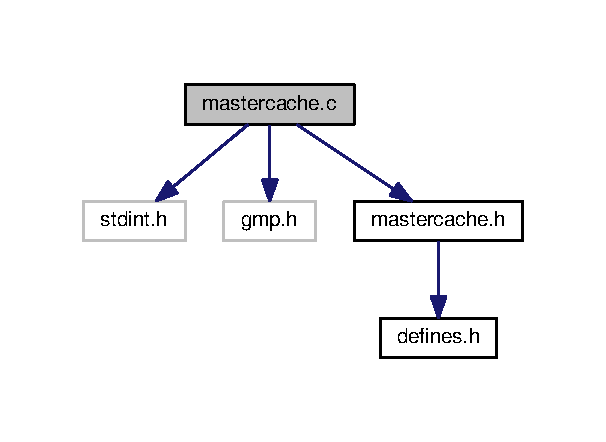
\includegraphics[width=291pt]{mastercache_8c__incl}
\end{center}
\end{figure}
\subsection*{Functions}
\begin{DoxyCompactItemize}
\item 
void \hyperlink{mastercache_8c_ad0254518fa335884d9330470e7889186}{cache\+\_\+init} (\hyperlink{structMasterCache}{Master\+Cache} $\ast$mstr, uint64\+\_\+t cache\+\_\+size)
\begin{DoxyCompactList}\small\item\em Init function for master cache. \end{DoxyCompactList}\item 
cached\+Int \hyperlink{mastercache_8c_a50d90b1940a54a27f5582e46f02483c2}{cache\+\_\+add} (\hyperlink{structMasterCache}{Master\+Cache} $\ast$mstr, mpz\+\_\+t new)
\begin{DoxyCompactList}\small\item\em add function for master cache \end{DoxyCompactList}\item 
bool \hyperlink{mastercache_8c_af3f696b0d56758825d872a5280bcfd7b}{cache\+\_\+exists} (\hyperlink{structMasterCache}{Master\+Cache} $\ast$mstr, mpz\+\_\+t element)
\begin{DoxyCompactList}\small\item\em function for master cache to check if an item exists \end{DoxyCompactList}\item 
void \hyperlink{mastercache_8c_acd42afe339ef9ef2a2c6c6733f870e07}{cache\+\_\+get} (\hyperlink{structMasterCache}{Master\+Cache} $\ast$mstr, cached\+Int element, mpz\+\_\+t result)
\begin{DoxyCompactList}\small\item\em function for master cache to get an item back from cache as mpq\+\_\+t \end{DoxyCompactList}\end{DoxyCompactItemize}


\subsection{Detailed Description}
Master Cache for caching Integers and Integer operations from gmp. 

\begin{DoxyAuthor}{Author}
Sandra Hicks 
\end{DoxyAuthor}


\subsection{Function Documentation}
\index{mastercache.\+c@{mastercache.\+c}!cache\+\_\+add@{cache\+\_\+add}}
\index{cache\+\_\+add@{cache\+\_\+add}!mastercache.\+c@{mastercache.\+c}}
\subsubsection[{\texorpdfstring{cache\+\_\+add(\+Master\+Cache $\ast$mstr, mpz\+\_\+t new)}{cache_add(MasterCache *mstr, mpz_t new)}}]{\setlength{\rightskip}{0pt plus 5cm}cached\+Int cache\+\_\+add (
\begin{DoxyParamCaption}
\item[{{\bf Master\+Cache} $\ast$}]{mstr, }
\item[{mpz\+\_\+t}]{new}
\end{DoxyParamCaption}
)}\hypertarget{mastercache_8c_a50d90b1940a54a27f5582e46f02483c2}{}\label{mastercache_8c_a50d90b1940a54a27f5582e46f02483c2}


add function for master cache 


\begin{DoxyParams}{Parameters}
{\em mstr} & \hyperlink{structMasterCache}{Master\+Cache} pointer \\
\hline
{\em new} & mpz\+\_\+t to be added to cache \\
\hline
\end{DoxyParams}
\index{mastercache.\+c@{mastercache.\+c}!cache\+\_\+exists@{cache\+\_\+exists}}
\index{cache\+\_\+exists@{cache\+\_\+exists}!mastercache.\+c@{mastercache.\+c}}
\subsubsection[{\texorpdfstring{cache\+\_\+exists(\+Master\+Cache $\ast$mstr, mpz\+\_\+t element)}{cache_exists(MasterCache *mstr, mpz_t element)}}]{\setlength{\rightskip}{0pt plus 5cm}bool cache\+\_\+exists (
\begin{DoxyParamCaption}
\item[{{\bf Master\+Cache} $\ast$}]{mstr, }
\item[{mpz\+\_\+t}]{element}
\end{DoxyParamCaption}
)}\hypertarget{mastercache_8c_af3f696b0d56758825d872a5280bcfd7b}{}\label{mastercache_8c_af3f696b0d56758825d872a5280bcfd7b}


function for master cache to check if an item exists 


\begin{DoxyParams}{Parameters}
{\em mstr} & \hyperlink{structMasterCache}{Master\+Cache} pointer \\
\hline
{\em element} & mpz\+\_\+t to be added to cache \\
\hline
\end{DoxyParams}
\index{mastercache.\+c@{mastercache.\+c}!cache\+\_\+get@{cache\+\_\+get}}
\index{cache\+\_\+get@{cache\+\_\+get}!mastercache.\+c@{mastercache.\+c}}
\subsubsection[{\texorpdfstring{cache\+\_\+get(\+Master\+Cache $\ast$mstr, cached\+Int element, mpz\+\_\+t result)}{cache_get(MasterCache *mstr, cachedInt element, mpz_t result)}}]{\setlength{\rightskip}{0pt plus 5cm}void cache\+\_\+get (
\begin{DoxyParamCaption}
\item[{{\bf Master\+Cache} $\ast$}]{mstr, }
\item[{cached\+Int}]{element, }
\item[{mpz\+\_\+t}]{result}
\end{DoxyParamCaption}
)}\hypertarget{mastercache_8c_acd42afe339ef9ef2a2c6c6733f870e07}{}\label{mastercache_8c_acd42afe339ef9ef2a2c6c6733f870e07}


function for master cache to get an item back from cache as mpq\+\_\+t 


\begin{DoxyParams}{Parameters}
{\em mstr} & \hyperlink{structMasterCache}{Master\+Cache} pointer \\
\hline
{\em element} & id of the element to get from cache \\
\hline
\end{DoxyParams}
\index{mastercache.\+c@{mastercache.\+c}!cache\+\_\+init@{cache\+\_\+init}}
\index{cache\+\_\+init@{cache\+\_\+init}!mastercache.\+c@{mastercache.\+c}}
\subsubsection[{\texorpdfstring{cache\+\_\+init(\+Master\+Cache $\ast$mstr, uint64\+\_\+t cache\+\_\+size)}{cache_init(MasterCache *mstr, uint64_t cache_size)}}]{\setlength{\rightskip}{0pt plus 5cm}void cache\+\_\+init (
\begin{DoxyParamCaption}
\item[{{\bf Master\+Cache} $\ast$}]{mstr, }
\item[{uint64\+\_\+t}]{cache\+\_\+size}
\end{DoxyParamCaption}
)}\hypertarget{mastercache_8c_ad0254518fa335884d9330470e7889186}{}\label{mastercache_8c_ad0254518fa335884d9330470e7889186}


Init function for master cache. 


\begin{DoxyParams}{Parameters}
{\em mstr} & \hyperlink{structMasterCache}{Master\+Cache} pointer to be initialized \\
\hline
{\em cache\+\_\+size} & size of the cache for mpz\+\_\+t \\
\hline
\end{DoxyParams}

\hypertarget{mastercache_8h}{}\section{mastercache.\+h File Reference}
\label{mastercache_8h}\index{mastercache.\+h@{mastercache.\+h}}


header for Master Cache for caching Integers and Integer operations from gmp.  


{\ttfamily \#include \char`\"{}defines.\+h\char`\"{}}\\*
{\ttfamily \#include \char`\"{}caching\+\_\+operations.\+h\char`\"{}}\\*
Include dependency graph for mastercache.\+h\+:\nopagebreak
\begin{figure}[H]
\begin{center}
\leavevmode
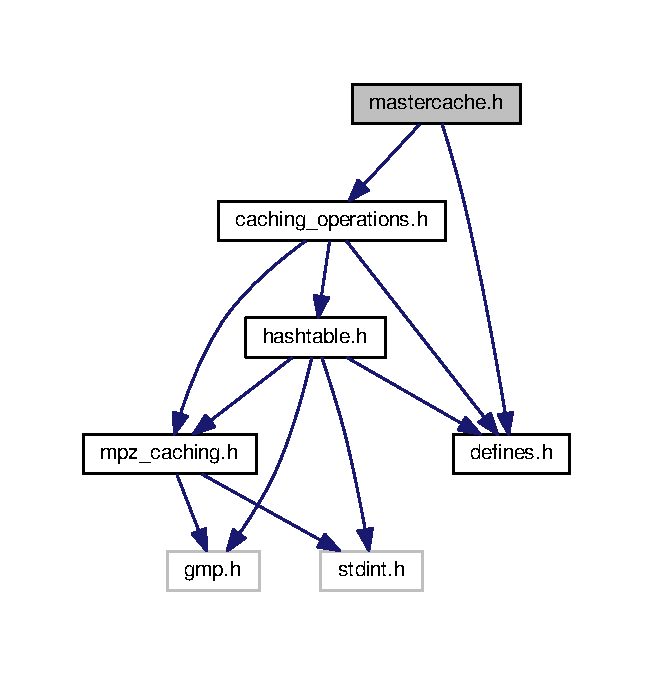
\includegraphics[width=314pt]{mastercache_8h__incl}
\end{center}
\end{figure}
This graph shows which files directly or indirectly include this file\+:\nopagebreak
\begin{figure}[H]
\begin{center}
\leavevmode
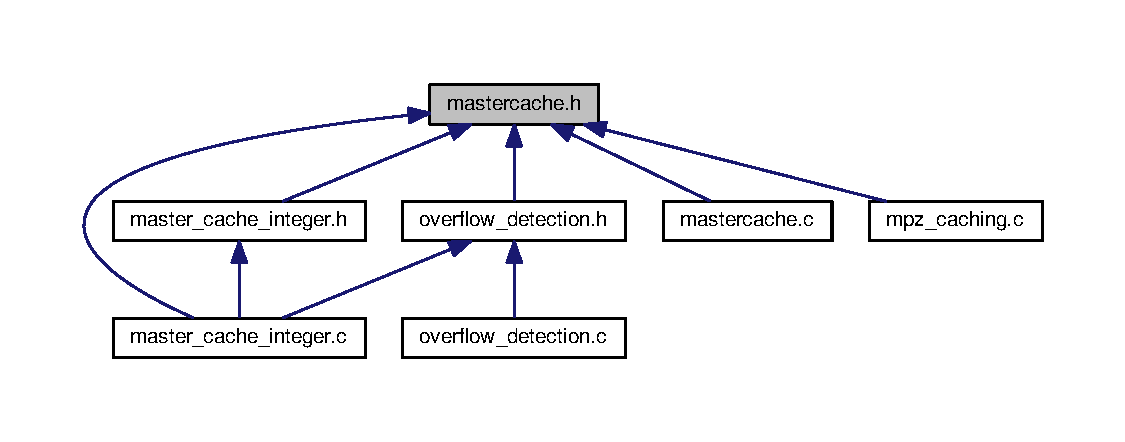
\includegraphics[width=350pt]{mastercache_8h__dep__incl}
\end{center}
\end{figure}
\subsection*{Classes}
\begin{DoxyCompactItemize}
\item 
struct \hyperlink{structMasterCacheInt}{Master\+Cache\+Int}
\item 
struct \hyperlink{structMasterCacheRational}{Master\+Cache\+Rational}
\item 
struct \hyperlink{structMasterCache}{Master\+Cache}
\begin{DoxyCompactList}\small\item\em \hyperlink{structMasterCache}{Master\+Cache}. \end{DoxyCompactList}\end{DoxyCompactItemize}
\subsection*{Typedefs}
\begin{DoxyCompactItemize}
\item 
typedef struct \hyperlink{structMasterCacheInt}{Master\+Cache\+Int} \hyperlink{mastercache_8h_a36a548913d4fa7ddfc3b5ab7bdc13ccd}{Master\+Cache\+Int}
\item 
typedef struct \hyperlink{structMasterCacheRational}{Master\+Cache\+Rational} \hyperlink{mastercache_8h_ae2ed1003e5fb6289d67ad8a4af2f8785}{Master\+Cache\+Rational}
\item 
typedef struct \hyperlink{structMasterCache}{Master\+Cache} \hyperlink{mastercache_8h_ad193fc2757a525675885e0a4cc7b01f4}{Master\+Cache}\hypertarget{mastercache_8h_ad193fc2757a525675885e0a4cc7b01f4}{}\label{mastercache_8h_ad193fc2757a525675885e0a4cc7b01f4}

\begin{DoxyCompactList}\small\item\em \hyperlink{structMasterCache}{Master\+Cache}. \end{DoxyCompactList}\item 
typedef uint64\+\_\+t \hyperlink{mastercache_8h_a113c03970467afb459ed5ae157d0a870}{cached\+Int}
\end{DoxyCompactItemize}


\subsection{Detailed Description}
header for Master Cache for caching Integers and Integer operations from gmp. 

\begin{DoxyAuthor}{Author}
Sandra Hicks 
\end{DoxyAuthor}


\subsection{Typedef Documentation}
\index{mastercache.\+h@{mastercache.\+h}!cached\+Int@{cached\+Int}}
\index{cached\+Int@{cached\+Int}!mastercache.\+h@{mastercache.\+h}}
\subsubsection[{\texorpdfstring{cached\+Int}{cachedInt}}]{\setlength{\rightskip}{0pt plus 5cm}typedef uint64\+\_\+t {\bf cached\+Int}}\hypertarget{mastercache_8h_a113c03970467afb459ed5ae157d0a870}{}\label{mastercache_8h_a113c03970467afb459ed5ae157d0a870}
cached\+Int can be either an id to a cached mpz\+\_\+t (indicated by M\+SB) or an actual number, the sign is indicated by M\+S\+B-\/1 \index{mastercache.\+h@{mastercache.\+h}!Master\+Cache\+Int@{Master\+Cache\+Int}}
\index{Master\+Cache\+Int@{Master\+Cache\+Int}!mastercache.\+h@{mastercache.\+h}}
\subsubsection[{\texorpdfstring{Master\+Cache\+Int}{MasterCacheInt}}]{\setlength{\rightskip}{0pt plus 5cm}typedef struct {\bf Master\+Cache\+Int}  {\bf Master\+Cache\+Int}}\hypertarget{mastercache_8h_a36a548913d4fa7ddfc3b5ab7bdc13ccd}{}\label{mastercache_8h_a36a548913d4fa7ddfc3b5ab7bdc13ccd}
Master cache for integers \index{mastercache.\+h@{mastercache.\+h}!Master\+Cache\+Rational@{Master\+Cache\+Rational}}
\index{Master\+Cache\+Rational@{Master\+Cache\+Rational}!mastercache.\+h@{mastercache.\+h}}
\subsubsection[{\texorpdfstring{Master\+Cache\+Rational}{MasterCacheRational}}]{\setlength{\rightskip}{0pt plus 5cm}typedef struct {\bf Master\+Cache\+Rational}  {\bf Master\+Cache\+Rational}}\hypertarget{mastercache_8h_ae2ed1003e5fb6289d67ad8a4af2f8785}{}\label{mastercache_8h_ae2ed1003e5fb6289d67ad8a4af2f8785}
Master cache for rationals 
\hypertarget{mpz__caching_8c}{}\section{mpz\+\_\+caching.\+c File Reference}
\label{mpz__caching_8c}\index{mpz\+\_\+caching.\+c@{mpz\+\_\+caching.\+c}}


cache  


{\ttfamily \#include \char`\"{}mpz\+\_\+caching.\+h\char`\"{}}\\*
{\ttfamily \#include \char`\"{}mastercache.\+h\char`\"{}}\\*
Include dependency graph for mpz\+\_\+caching.\+c\+:
\nopagebreak
\begin{figure}[H]
\begin{center}
\leavevmode
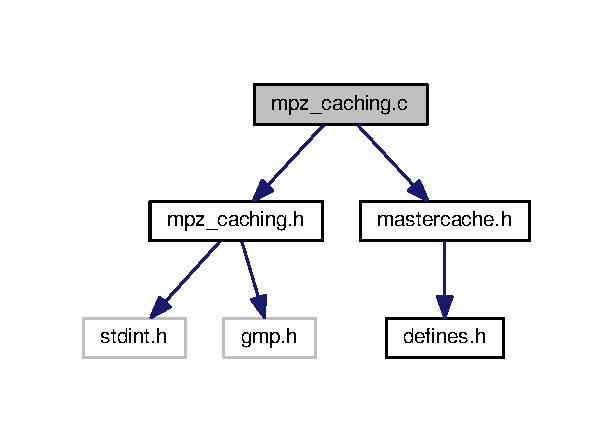
\includegraphics[width=294pt]{mpz__caching_8c__incl}
\end{center}
\end{figure}
\subsection*{Functions}
\begin{DoxyCompactItemize}
\item 
void {\bfseries init\+\_\+mpz\+\_\+cache} (int64\+\_\+t size, \hyperlink{structcached__mpz__t}{cached\+\_\+mpz\+\_\+t} $\ast$result)\hypertarget{mpz__caching_8c_a109c49f18d6466a6ede1e21ac45f090c}{}\label{mpz__caching_8c_a109c49f18d6466a6ede1e21ac45f090c}

\end{DoxyCompactItemize}


\subsection{Detailed Description}
cache 

\begin{DoxyAuthor}{Author}
Sandra Hicks 
\end{DoxyAuthor}

\hypertarget{mpz__caching_8h}{}\section{mpz\+\_\+caching.\+h File Reference}
\label{mpz__caching_8h}\index{mpz\+\_\+caching.\+h@{mpz\+\_\+caching.\+h}}


header for cache for mpz\+\_\+t  


{\ttfamily \#include $<$stdint.\+h$>$}\\*
{\ttfamily \#include $<$gmp.\+h$>$}\\*
Include dependency graph for mpz\+\_\+caching.\+h\+:\nopagebreak
\begin{figure}[H]
\begin{center}
\leavevmode
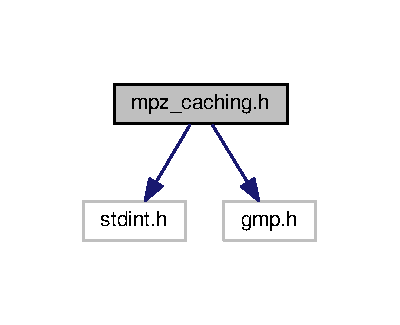
\includegraphics[width=192pt]{mpz__caching_8h__incl}
\end{center}
\end{figure}
This graph shows which files directly or indirectly include this file\+:\nopagebreak
\begin{figure}[H]
\begin{center}
\leavevmode
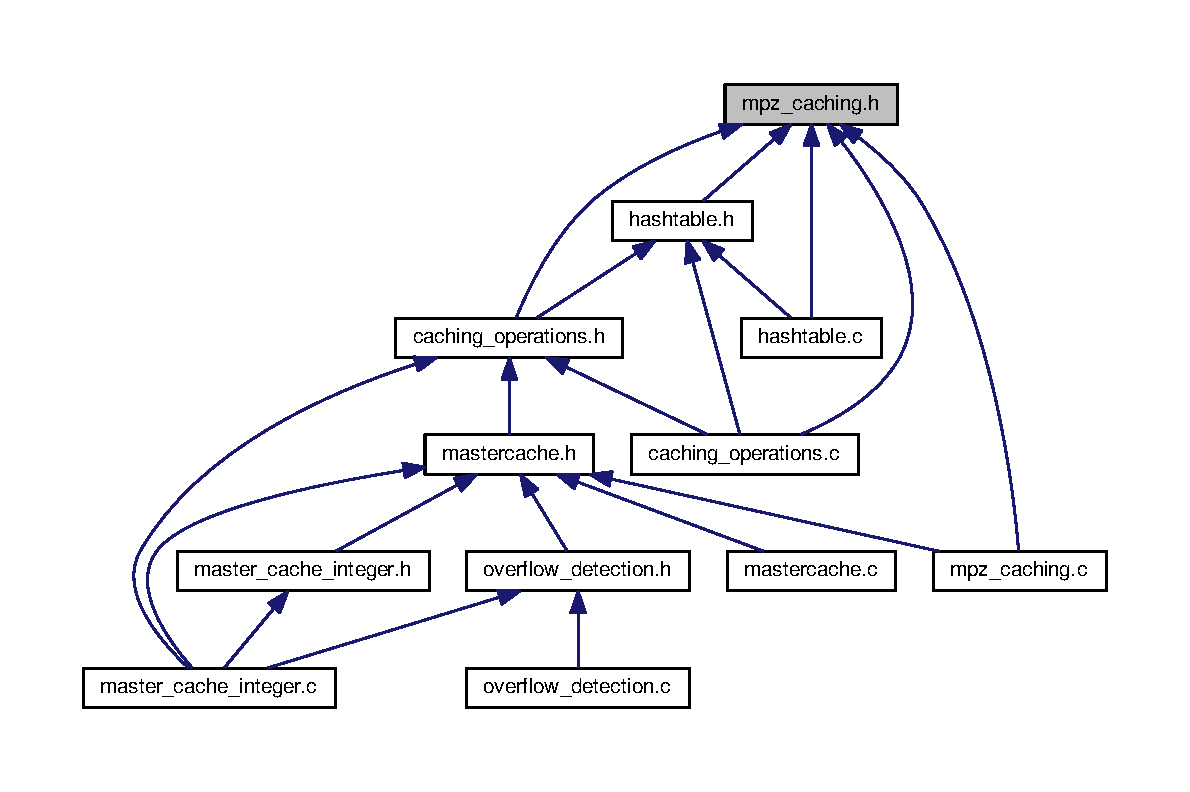
\includegraphics[width=350pt]{mpz__caching_8h__dep__incl}
\end{center}
\end{figure}
\subsection*{Classes}
\begin{DoxyCompactItemize}
\item 
struct \hyperlink{structcached__mpz__t}{cached\+\_\+mpz\+\_\+t}
\begin{DoxyCompactList}\small\item\em cached representation of an mpz\+\_\+t \end{DoxyCompactList}\item 
struct \hyperlink{structmpz__t__cache}{mpz\+\_\+t\+\_\+cache}
\begin{DoxyCompactList}\small\item\em cache implemented as an array (fast random access) \end{DoxyCompactList}\end{DoxyCompactItemize}
\subsection*{Typedefs}
\begin{DoxyCompactItemize}
\item 
typedef struct \hyperlink{structcached__mpz__t}{cached\+\_\+mpz\+\_\+t} \hyperlink{mpz__caching_8h_a43691d5ed6539a74f75fcbb2eeb01d8e}{cached\+\_\+mpz\+\_\+t}\hypertarget{mpz__caching_8h_a43691d5ed6539a74f75fcbb2eeb01d8e}{}\label{mpz__caching_8h_a43691d5ed6539a74f75fcbb2eeb01d8e}

\begin{DoxyCompactList}\small\item\em cached representation of an mpz\+\_\+t \end{DoxyCompactList}\item 
typedef struct \hyperlink{structmpz__t__cache}{mpz\+\_\+t\+\_\+cache} \hyperlink{mpz__caching_8h_a084f99de7821a83cdca8d0f747cd6484}{mpz\+\_\+t\+\_\+cache}\hypertarget{mpz__caching_8h_a084f99de7821a83cdca8d0f747cd6484}{}\label{mpz__caching_8h_a084f99de7821a83cdca8d0f747cd6484}

\begin{DoxyCompactList}\small\item\em cache implemented as an array (fast random access) \end{DoxyCompactList}\end{DoxyCompactItemize}
\subsection*{Functions}
\begin{DoxyCompactItemize}
\item 
void \hyperlink{mpz__caching_8h_af5387ca483d290f5da20649239c5fdef}{init\+\_\+mpz\+\_\+cache} (\hyperlink{structmpz__t__cache}{mpz\+\_\+t\+\_\+cache} $\ast$cache, uint64\+\_\+t size)
\begin{DoxyCompactList}\small\item\em initialization of the cache \end{DoxyCompactList}\item 
void \hyperlink{mpz__caching_8h_aad2ec516965e5bd06eb4ed91a9707775}{delete\+\_\+mpz\+\_\+cache} (\hyperlink{structmpz__t__cache}{mpz\+\_\+t\+\_\+cache} $\ast$cache)
\begin{DoxyCompactList}\small\item\em deletion of the cache and free of all underlying data structures \end{DoxyCompactList}\item 
int64\+\_\+t \hyperlink{mpz__caching_8h_ab93e1f89e6a97ba347b58bd7955d02ba}{insert\+\_\+mpz} (\hyperlink{structmpz__t__cache}{mpz\+\_\+t\+\_\+cache} $\ast$cache, mpz\+\_\+t val)
\begin{DoxyCompactList}\small\item\em insert a new mpz\+\_\+t in cache, no check for double, start at id=1 (0 is reserved for errors) \end{DoxyCompactList}\item 
void \hyperlink{mpz__caching_8h_a4ea9e1949f05c8ed0fa17421e156d7ba}{print\+Entry} (\hyperlink{structmpz__t__cache}{mpz\+\_\+t\+\_\+cache} $\ast$cache, uint64\+\_\+t i)
\begin{DoxyCompactList}\small\item\em print function for debugging, prints double representation \end{DoxyCompactList}\item 
void \hyperlink{mpz__caching_8h_acfb7f476b995041bb4ba41e31f5220ae}{get\+\_\+cached\+\_\+mpz} (\hyperlink{structmpz__t__cache}{mpz\+\_\+t\+\_\+cache} $\ast$cache, uint64\+\_\+t i, mpz\+\_\+t val)
\begin{DoxyCompactList}\small\item\em get a cached mpz\+\_\+t by id \end{DoxyCompactList}\item 
double \hyperlink{mpz__caching_8h_a1afc9ada65a26e6562e7eb6b24064f72}{get\+\_\+cached\+\_\+double} (\hyperlink{structmpz__t__cache}{mpz\+\_\+t\+\_\+cache} $\ast$cache, uint64\+\_\+t i)
\begin{DoxyCompactList}\small\item\em get double representation of a cached mpz\+\_\+t by id \end{DoxyCompactList}\end{DoxyCompactItemize}


\subsection{Detailed Description}
header for cache for mpz\+\_\+t 

\begin{DoxyAuthor}{Author}
Sandra Hicks 
\end{DoxyAuthor}


\subsection{Function Documentation}
\index{mpz\+\_\+caching.\+h@{mpz\+\_\+caching.\+h}!delete\+\_\+mpz\+\_\+cache@{delete\+\_\+mpz\+\_\+cache}}
\index{delete\+\_\+mpz\+\_\+cache@{delete\+\_\+mpz\+\_\+cache}!mpz\+\_\+caching.\+h@{mpz\+\_\+caching.\+h}}
\subsubsection[{\texorpdfstring{delete\+\_\+mpz\+\_\+cache(mpz\+\_\+t\+\_\+cache $\ast$cache)}{delete_mpz_cache(mpz_t_cache *cache)}}]{\setlength{\rightskip}{0pt plus 5cm}void delete\+\_\+mpz\+\_\+cache (
\begin{DoxyParamCaption}
\item[{{\bf mpz\+\_\+t\+\_\+cache} $\ast$}]{cache}
\end{DoxyParamCaption}
)}\hypertarget{mpz__caching_8h_aad2ec516965e5bd06eb4ed91a9707775}{}\label{mpz__caching_8h_aad2ec516965e5bd06eb4ed91a9707775}


deletion of the cache and free of all underlying data structures 


\begin{DoxyParams}{Parameters}
{\em cache} & pointer to cache \\
\hline
\end{DoxyParams}
\index{mpz\+\_\+caching.\+h@{mpz\+\_\+caching.\+h}!get\+\_\+cached\+\_\+double@{get\+\_\+cached\+\_\+double}}
\index{get\+\_\+cached\+\_\+double@{get\+\_\+cached\+\_\+double}!mpz\+\_\+caching.\+h@{mpz\+\_\+caching.\+h}}
\subsubsection[{\texorpdfstring{get\+\_\+cached\+\_\+double(mpz\+\_\+t\+\_\+cache $\ast$cache, uint64\+\_\+t i)}{get_cached_double(mpz_t_cache *cache, uint64_t i)}}]{\setlength{\rightskip}{0pt plus 5cm}double get\+\_\+cached\+\_\+double (
\begin{DoxyParamCaption}
\item[{{\bf mpz\+\_\+t\+\_\+cache} $\ast$}]{cache, }
\item[{uint64\+\_\+t}]{i}
\end{DoxyParamCaption}
)}\hypertarget{mpz__caching_8h_a1afc9ada65a26e6562e7eb6b24064f72}{}\label{mpz__caching_8h_a1afc9ada65a26e6562e7eb6b24064f72}


get double representation of a cached mpz\+\_\+t by id 


\begin{DoxyParams}{Parameters}
{\em cache} & pointer to cache \\
\hline
{\em i} & requested id \\
\hline
\end{DoxyParams}
\begin{DoxyReturn}{Returns}
double representation 
\end{DoxyReturn}
\index{mpz\+\_\+caching.\+h@{mpz\+\_\+caching.\+h}!get\+\_\+cached\+\_\+mpz@{get\+\_\+cached\+\_\+mpz}}
\index{get\+\_\+cached\+\_\+mpz@{get\+\_\+cached\+\_\+mpz}!mpz\+\_\+caching.\+h@{mpz\+\_\+caching.\+h}}
\subsubsection[{\texorpdfstring{get\+\_\+cached\+\_\+mpz(mpz\+\_\+t\+\_\+cache $\ast$cache, uint64\+\_\+t i, mpz\+\_\+t val)}{get_cached_mpz(mpz_t_cache *cache, uint64_t i, mpz_t val)}}]{\setlength{\rightskip}{0pt plus 5cm}void get\+\_\+cached\+\_\+mpz (
\begin{DoxyParamCaption}
\item[{{\bf mpz\+\_\+t\+\_\+cache} $\ast$}]{cache, }
\item[{uint64\+\_\+t}]{i, }
\item[{mpz\+\_\+t}]{val}
\end{DoxyParamCaption}
)}\hypertarget{mpz__caching_8h_acfb7f476b995041bb4ba41e31f5220ae}{}\label{mpz__caching_8h_acfb7f476b995041bb4ba41e31f5220ae}


get a cached mpz\+\_\+t by id 


\begin{DoxyParams}{Parameters}
{\em cache} & pointer to cache \\
\hline
{\em i} & requested id \\
\hline
{\em val} & mpz\+\_\+t to set for return \\
\hline
\end{DoxyParams}
\index{mpz\+\_\+caching.\+h@{mpz\+\_\+caching.\+h}!init\+\_\+mpz\+\_\+cache@{init\+\_\+mpz\+\_\+cache}}
\index{init\+\_\+mpz\+\_\+cache@{init\+\_\+mpz\+\_\+cache}!mpz\+\_\+caching.\+h@{mpz\+\_\+caching.\+h}}
\subsubsection[{\texorpdfstring{init\+\_\+mpz\+\_\+cache(mpz\+\_\+t\+\_\+cache $\ast$cache, uint64\+\_\+t size)}{init_mpz_cache(mpz_t_cache *cache, uint64_t size)}}]{\setlength{\rightskip}{0pt plus 5cm}void init\+\_\+mpz\+\_\+cache (
\begin{DoxyParamCaption}
\item[{{\bf mpz\+\_\+t\+\_\+cache} $\ast$}]{cache, }
\item[{uint64\+\_\+t}]{size}
\end{DoxyParamCaption}
)}\hypertarget{mpz__caching_8h_af5387ca483d290f5da20649239c5fdef}{}\label{mpz__caching_8h_af5387ca483d290f5da20649239c5fdef}


initialization of the cache 


\begin{DoxyParams}{Parameters}
{\em cache} & pointer to cache \\
\hline
{\em size} & initial size of the cache \\
\hline
\end{DoxyParams}
\index{mpz\+\_\+caching.\+h@{mpz\+\_\+caching.\+h}!insert\+\_\+mpz@{insert\+\_\+mpz}}
\index{insert\+\_\+mpz@{insert\+\_\+mpz}!mpz\+\_\+caching.\+h@{mpz\+\_\+caching.\+h}}
\subsubsection[{\texorpdfstring{insert\+\_\+mpz(mpz\+\_\+t\+\_\+cache $\ast$cache, mpz\+\_\+t val)}{insert_mpz(mpz_t_cache *cache, mpz_t val)}}]{\setlength{\rightskip}{0pt plus 5cm}int64\+\_\+t insert\+\_\+mpz (
\begin{DoxyParamCaption}
\item[{{\bf mpz\+\_\+t\+\_\+cache} $\ast$}]{cache, }
\item[{mpz\+\_\+t}]{val}
\end{DoxyParamCaption}
)}\hypertarget{mpz__caching_8h_ab93e1f89e6a97ba347b58bd7955d02ba}{}\label{mpz__caching_8h_ab93e1f89e6a97ba347b58bd7955d02ba}


insert a new mpz\+\_\+t in cache, no check for double, start at id=1 (0 is reserved for errors) 


\begin{DoxyParams}{Parameters}
{\em cache} & pointer to cache \\
\hline
{\em val} & mpz\+\_\+t to insert \\
\hline
\end{DoxyParams}
\begin{DoxyReturn}{Returns}
id of inserted element 
\end{DoxyReturn}
\index{mpz\+\_\+caching.\+h@{mpz\+\_\+caching.\+h}!print\+Entry@{print\+Entry}}
\index{print\+Entry@{print\+Entry}!mpz\+\_\+caching.\+h@{mpz\+\_\+caching.\+h}}
\subsubsection[{\texorpdfstring{print\+Entry(mpz\+\_\+t\+\_\+cache $\ast$cache, uint64\+\_\+t i)}{printEntry(mpz_t_cache *cache, uint64_t i)}}]{\setlength{\rightskip}{0pt plus 5cm}void print\+Entry (
\begin{DoxyParamCaption}
\item[{{\bf mpz\+\_\+t\+\_\+cache} $\ast$}]{cache, }
\item[{uint64\+\_\+t}]{i}
\end{DoxyParamCaption}
)}\hypertarget{mpz__caching_8h_a4ea9e1949f05c8ed0fa17421e156d7ba}{}\label{mpz__caching_8h_a4ea9e1949f05c8ed0fa17421e156d7ba}


print function for debugging, prints double representation 


\begin{DoxyParams}{Parameters}
{\em cache} & \\
\hline
{\em i} & id \\
\hline
\end{DoxyParams}

\hypertarget{overflow__detection_8c}{}\section{overflow\+\_\+detection.\+c File Reference}
\label{overflow__detection_8c}\index{overflow\+\_\+detection.\+c@{overflow\+\_\+detection.\+c}}


Functions to detect overflows in integer operations.  


{\ttfamily \#include $<$stdint.\+h$>$}\\*
{\ttfamily \#include \char`\"{}overflow\+\_\+detection.\+h\char`\"{}}\\*
{\ttfamily \#include \char`\"{}defines.\+h\char`\"{}}\\*
{\ttfamily \#include $<$stdio.\+h$>$}\\*
{\ttfamily \#include $<$inttypes.\+h$>$}\\*
Include dependency graph for overflow\+\_\+detection.\+c\+:\nopagebreak
\begin{figure}[H]
\begin{center}
\leavevmode
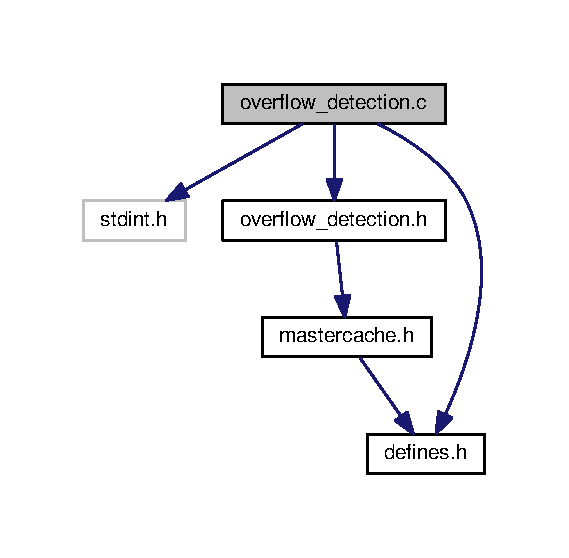
\includegraphics[width=350pt]{overflow__detection_8c__incl}
\end{center}
\end{figure}
\subsection*{Macros}
\begin{DoxyCompactItemize}
\item 
\#define \hyperlink{overflow__detection_8c_af3694ae57103552f7fba8b94e114a90f}{M\+A\+X\+B\+IT}~62
\end{DoxyCompactItemize}
\subsection*{Functions}
\begin{DoxyCompactItemize}
\item 
uint32\+\_\+t \hyperlink{overflow__detection_8c_ab9ebfca4f389fbfd7518c73802739dfa}{M\+SB} (\hyperlink{mastercache_8h_a113c03970467afb459ed5ae157d0a870}{cached\+Int} val)
\item 
\hyperlink{mastercache_8h_a113c03970467afb459ed5ae157d0a870}{cached\+Int} \hyperlink{overflow__detection_8c_a069c125ad06465b64cbfe809b29ec9ce}{delete\+Id\+Bit} (\hyperlink{mastercache_8h_a113c03970467afb459ed5ae157d0a870}{cached\+Int} val)
\item 
int \hyperlink{overflow__detection_8c_a9353ddb1f8619095dfce206ab4209d3a}{addition\+Overflow} (\hyperlink{mastercache_8h_a113c03970467afb459ed5ae157d0a870}{cached\+Int} op1, \hyperlink{mastercache_8h_a113c03970467afb459ed5ae157d0a870}{cached\+Int} op2)
\begin{DoxyCompactList}\small\item\em function to predict if an addition will overflow \end{DoxyCompactList}\item 
int \hyperlink{overflow__detection_8c_a3d152657eff6ecfd62713f7252beb0fe}{multiplication\+Overflow} (\hyperlink{mastercache_8h_a113c03970467afb459ed5ae157d0a870}{cached\+Int} op1, \hyperlink{mastercache_8h_a113c03970467afb459ed5ae157d0a870}{cached\+Int} op2)
\begin{DoxyCompactList}\small\item\em function to predict if a multiplication will overflow \end{DoxyCompactList}\item 
int \hyperlink{overflow__detection_8c_a3f5d390da9ae4425c7ba83964f3b0905}{exponentiation\+Overflow} (\hyperlink{mastercache_8h_a113c03970467afb459ed5ae157d0a870}{cached\+Int} base, \hyperlink{mastercache_8h_a113c03970467afb459ed5ae157d0a870}{cached\+Int} exp)
\begin{DoxyCompactList}\small\item\em function to predict if an exponentiation will overflow \end{DoxyCompactList}\end{DoxyCompactItemize}


\subsection{Detailed Description}
Functions to detect overflows in integer operations. 

\begin{DoxyAuthor}{Author}
Sandra Hicks 
\end{DoxyAuthor}


\subsection{Macro Definition Documentation}
\index{overflow\+\_\+detection.\+c@{overflow\+\_\+detection.\+c}!M\+A\+X\+B\+IT@{M\+A\+X\+B\+IT}}
\index{M\+A\+X\+B\+IT@{M\+A\+X\+B\+IT}!overflow\+\_\+detection.\+c@{overflow\+\_\+detection.\+c}}
\subsubsection[{\texorpdfstring{M\+A\+X\+B\+IT}{MAXBIT}}]{\setlength{\rightskip}{0pt plus 5cm}\#define M\+A\+X\+B\+IT~62}\hypertarget{overflow__detection_8c_af3694ae57103552f7fba8b94e114a90f}{}\label{overflow__detection_8c_af3694ae57103552f7fba8b94e114a90f}
maximal bit to be set before overflow 

\subsection{Function Documentation}
\index{overflow\+\_\+detection.\+c@{overflow\+\_\+detection.\+c}!addition\+Overflow@{addition\+Overflow}}
\index{addition\+Overflow@{addition\+Overflow}!overflow\+\_\+detection.\+c@{overflow\+\_\+detection.\+c}}
\subsubsection[{\texorpdfstring{addition\+Overflow(cached\+Int op1, cached\+Int op2)}{additionOverflow(cachedInt op1, cachedInt op2)}}]{\setlength{\rightskip}{0pt plus 5cm}int addition\+Overflow (
\begin{DoxyParamCaption}
\item[{{\bf cached\+Int}}]{op1, }
\item[{{\bf cached\+Int}}]{op2}
\end{DoxyParamCaption}
)}\hypertarget{overflow__detection_8c_a9353ddb1f8619095dfce206ab4209d3a}{}\label{overflow__detection_8c_a9353ddb1f8619095dfce206ab4209d3a}


function to predict if an addition will overflow 


\begin{DoxyParams}{Parameters}
{\em op1} & first operator \\
\hline
{\em op2} & second operator \\
\hline
\end{DoxyParams}
\index{overflow\+\_\+detection.\+c@{overflow\+\_\+detection.\+c}!delete\+Id\+Bit@{delete\+Id\+Bit}}
\index{delete\+Id\+Bit@{delete\+Id\+Bit}!overflow\+\_\+detection.\+c@{overflow\+\_\+detection.\+c}}
\subsubsection[{\texorpdfstring{delete\+Id\+Bit(cached\+Int val)}{deleteIdBit(cachedInt val)}}]{\setlength{\rightskip}{0pt plus 5cm}{\bf cached\+Int} delete\+Id\+Bit (
\begin{DoxyParamCaption}
\item[{{\bf cached\+Int}}]{val}
\end{DoxyParamCaption}
)}\hypertarget{overflow__detection_8c_a069c125ad06465b64cbfe809b29ec9ce}{}\label{overflow__detection_8c_a069c125ad06465b64cbfe809b29ec9ce}
(for internal use only!) 
\begin{DoxyParams}{Parameters}
{\em val} & \\
\hline
\end{DoxyParams}
\begin{DoxyReturn}{Returns}

\end{DoxyReturn}
\index{overflow\+\_\+detection.\+c@{overflow\+\_\+detection.\+c}!exponentiation\+Overflow@{exponentiation\+Overflow}}
\index{exponentiation\+Overflow@{exponentiation\+Overflow}!overflow\+\_\+detection.\+c@{overflow\+\_\+detection.\+c}}
\subsubsection[{\texorpdfstring{exponentiation\+Overflow(cached\+Int base, cached\+Int exp)}{exponentiationOverflow(cachedInt base, cachedInt exp)}}]{\setlength{\rightskip}{0pt plus 5cm}int exponentiation\+Overflow (
\begin{DoxyParamCaption}
\item[{{\bf cached\+Int}}]{base, }
\item[{{\bf cached\+Int}}]{exp}
\end{DoxyParamCaption}
)}\hypertarget{overflow__detection_8c_a3f5d390da9ae4425c7ba83964f3b0905}{}\label{overflow__detection_8c_a3f5d390da9ae4425c7ba83964f3b0905}


function to predict if an exponentiation will overflow 


\begin{DoxyParams}{Parameters}
{\em base} & first operator, base \\
\hline
{\em exp} & second operator, exponent \\
\hline
\end{DoxyParams}
\index{overflow\+\_\+detection.\+c@{overflow\+\_\+detection.\+c}!M\+SB@{M\+SB}}
\index{M\+SB@{M\+SB}!overflow\+\_\+detection.\+c@{overflow\+\_\+detection.\+c}}
\subsubsection[{\texorpdfstring{M\+S\+B(cached\+Int val)}{MSB(cachedInt val)}}]{\setlength{\rightskip}{0pt plus 5cm}uint32\+\_\+t M\+SB (
\begin{DoxyParamCaption}
\item[{{\bf cached\+Int}}]{val}
\end{DoxyParamCaption}
)}\hypertarget{overflow__detection_8c_ab9ebfca4f389fbfd7518c73802739dfa}{}\label{overflow__detection_8c_ab9ebfca4f389fbfd7518c73802739dfa}
(for internal use only!) 
\begin{DoxyParams}{Parameters}
{\em val} & \\
\hline
\end{DoxyParams}
\begin{DoxyReturn}{Returns}

\end{DoxyReturn}
\index{overflow\+\_\+detection.\+c@{overflow\+\_\+detection.\+c}!multiplication\+Overflow@{multiplication\+Overflow}}
\index{multiplication\+Overflow@{multiplication\+Overflow}!overflow\+\_\+detection.\+c@{overflow\+\_\+detection.\+c}}
\subsubsection[{\texorpdfstring{multiplication\+Overflow(cached\+Int op1, cached\+Int op2)}{multiplicationOverflow(cachedInt op1, cachedInt op2)}}]{\setlength{\rightskip}{0pt plus 5cm}int multiplication\+Overflow (
\begin{DoxyParamCaption}
\item[{{\bf cached\+Int}}]{op1, }
\item[{{\bf cached\+Int}}]{op2}
\end{DoxyParamCaption}
)}\hypertarget{overflow__detection_8c_a3d152657eff6ecfd62713f7252beb0fe}{}\label{overflow__detection_8c_a3d152657eff6ecfd62713f7252beb0fe}


function to predict if a multiplication will overflow 


\begin{DoxyParams}{Parameters}
{\em op1} & first operator \\
\hline
{\em op2} & second operator \\
\hline
\end{DoxyParams}

\hypertarget{overflow__detection_8h}{}\section{overflow\+\_\+detection.\+h File Reference}
\label{overflow__detection_8h}\index{overflow\+\_\+detection.\+h@{overflow\+\_\+detection.\+h}}


header for overflow detection functions  


{\ttfamily \#include \char`\"{}mastercache.\+h\char`\"{}}\\*
Include dependency graph for overflow\+\_\+detection.\+h\+:\nopagebreak
\begin{figure}[H]
\begin{center}
\leavevmode
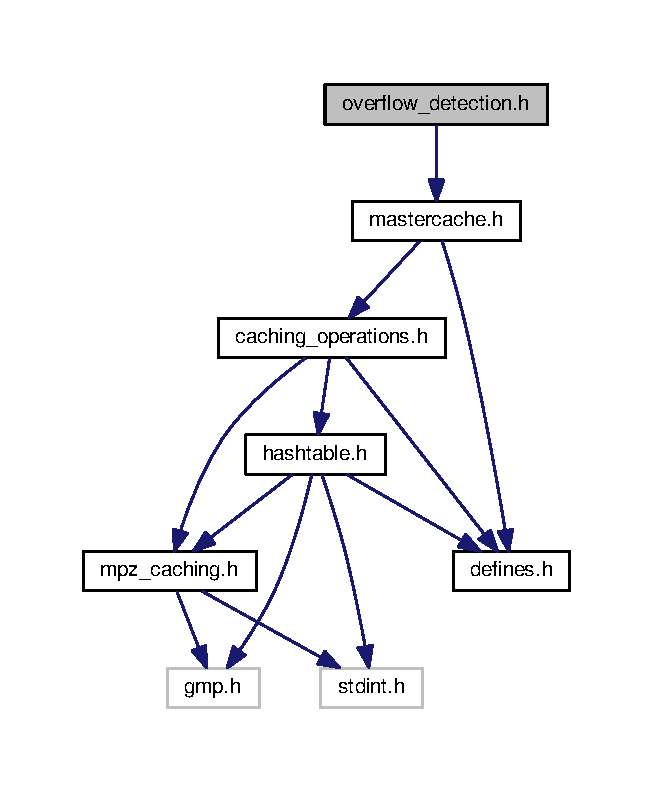
\includegraphics[width=314pt]{overflow__detection_8h__incl}
\end{center}
\end{figure}
This graph shows which files directly or indirectly include this file\+:\nopagebreak
\begin{figure}[H]
\begin{center}
\leavevmode
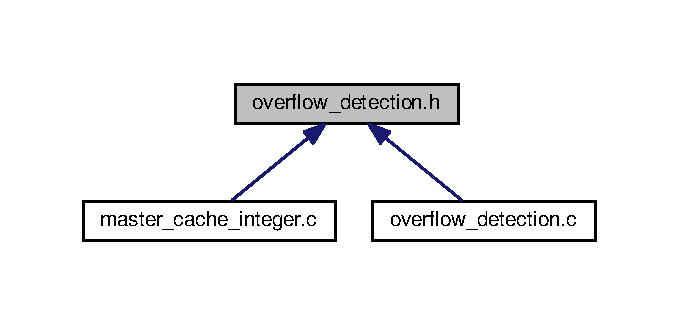
\includegraphics[width=326pt]{overflow__detection_8h__dep__incl}
\end{center}
\end{figure}
\subsection*{Functions}
\begin{DoxyCompactItemize}
\item 
int \hyperlink{overflow__detection_8h_a9353ddb1f8619095dfce206ab4209d3a}{addition\+Overflow} (\hyperlink{mastercache_8h_a113c03970467afb459ed5ae157d0a870}{cached\+Int} op1, \hyperlink{mastercache_8h_a113c03970467afb459ed5ae157d0a870}{cached\+Int} op2)
\begin{DoxyCompactList}\small\item\em function to predict if an addition will overflow \end{DoxyCompactList}\item 
int \hyperlink{overflow__detection_8h_a3d152657eff6ecfd62713f7252beb0fe}{multiplication\+Overflow} (\hyperlink{mastercache_8h_a113c03970467afb459ed5ae157d0a870}{cached\+Int} op1, \hyperlink{mastercache_8h_a113c03970467afb459ed5ae157d0a870}{cached\+Int} op2)
\begin{DoxyCompactList}\small\item\em function to predict if a multiplication will overflow \end{DoxyCompactList}\item 
int \hyperlink{overflow__detection_8h_a3f5d390da9ae4425c7ba83964f3b0905}{exponentiation\+Overflow} (\hyperlink{mastercache_8h_a113c03970467afb459ed5ae157d0a870}{cached\+Int} base, \hyperlink{mastercache_8h_a113c03970467afb459ed5ae157d0a870}{cached\+Int} exp)
\begin{DoxyCompactList}\small\item\em function to predict if an exponentiation will overflow \end{DoxyCompactList}\end{DoxyCompactItemize}


\subsection{Detailed Description}
header for overflow detection functions 

\begin{DoxyAuthor}{Author}
Sandra Hicks 
\end{DoxyAuthor}


\subsection{Function Documentation}
\index{overflow\+\_\+detection.\+h@{overflow\+\_\+detection.\+h}!addition\+Overflow@{addition\+Overflow}}
\index{addition\+Overflow@{addition\+Overflow}!overflow\+\_\+detection.\+h@{overflow\+\_\+detection.\+h}}
\subsubsection[{\texorpdfstring{addition\+Overflow(cached\+Int op1, cached\+Int op2)}{additionOverflow(cachedInt op1, cachedInt op2)}}]{\setlength{\rightskip}{0pt plus 5cm}int addition\+Overflow (
\begin{DoxyParamCaption}
\item[{{\bf cached\+Int}}]{op1, }
\item[{{\bf cached\+Int}}]{op2}
\end{DoxyParamCaption}
)}\hypertarget{overflow__detection_8h_a9353ddb1f8619095dfce206ab4209d3a}{}\label{overflow__detection_8h_a9353ddb1f8619095dfce206ab4209d3a}


function to predict if an addition will overflow 


\begin{DoxyParams}{Parameters}
{\em op1} & first operator \\
\hline
{\em op2} & second operator \\
\hline
\end{DoxyParams}
\index{overflow\+\_\+detection.\+h@{overflow\+\_\+detection.\+h}!exponentiation\+Overflow@{exponentiation\+Overflow}}
\index{exponentiation\+Overflow@{exponentiation\+Overflow}!overflow\+\_\+detection.\+h@{overflow\+\_\+detection.\+h}}
\subsubsection[{\texorpdfstring{exponentiation\+Overflow(cached\+Int base, cached\+Int exp)}{exponentiationOverflow(cachedInt base, cachedInt exp)}}]{\setlength{\rightskip}{0pt plus 5cm}int exponentiation\+Overflow (
\begin{DoxyParamCaption}
\item[{{\bf cached\+Int}}]{base, }
\item[{{\bf cached\+Int}}]{exp}
\end{DoxyParamCaption}
)}\hypertarget{overflow__detection_8h_a3f5d390da9ae4425c7ba83964f3b0905}{}\label{overflow__detection_8h_a3f5d390da9ae4425c7ba83964f3b0905}


function to predict if an exponentiation will overflow 


\begin{DoxyParams}{Parameters}
{\em base} & first operator, base \\
\hline
{\em exp} & second operator, exponent \\
\hline
\end{DoxyParams}
\index{overflow\+\_\+detection.\+h@{overflow\+\_\+detection.\+h}!multiplication\+Overflow@{multiplication\+Overflow}}
\index{multiplication\+Overflow@{multiplication\+Overflow}!overflow\+\_\+detection.\+h@{overflow\+\_\+detection.\+h}}
\subsubsection[{\texorpdfstring{multiplication\+Overflow(cached\+Int op1, cached\+Int op2)}{multiplicationOverflow(cachedInt op1, cachedInt op2)}}]{\setlength{\rightskip}{0pt plus 5cm}int multiplication\+Overflow (
\begin{DoxyParamCaption}
\item[{{\bf cached\+Int}}]{op1, }
\item[{{\bf cached\+Int}}]{op2}
\end{DoxyParamCaption}
)}\hypertarget{overflow__detection_8h_a3d152657eff6ecfd62713f7252beb0fe}{}\label{overflow__detection_8h_a3d152657eff6ecfd62713f7252beb0fe}


function to predict if a multiplication will overflow 


\begin{DoxyParams}{Parameters}
{\em op1} & first operator \\
\hline
{\em op2} & second operator \\
\hline
\end{DoxyParams}

%--- End generated contents ---

% Index
\backmatter
\newpage
\phantomsection
\clearemptydoublepage
\addcontentsline{toc}{chapter}{Index}
\printindex

\end{document}
